% Functional Collapse Without a Spectral Signature: SVD Dynamics of LoRA
% Adapters for Low-Resource Turkic Languages
% Anonymous ARR Submission

\documentclass[11pt]{article}
\usepackage{acl}
\usepackage{fontspec}
\usepackage{latexsym}
\newfontfamily\cyrfont{Noto Serif}
\usepackage{amsmath}
\usepackage{amssymb}
\usepackage{graphicx}
\usepackage{booktabs}
\usepackage{multirow}
\usepackage[table]{xcolor}
\usepackage{hyperref}
\usepackage{cleveref}

\title{Spectral Energy is Not a Reliable Collapse Diagnostic for Low-Resource Quantized LoRA: Evidence from Turkic Languages}

\author{Anonymous ARR Submission}

\begin{document}
\maketitle

% ============================================================================
% ABSTRACT
% ============================================================================
\begin{abstract}
We study the SVD and directional dynamics of LoRA adapters fine-tuned on three low-resource Turkic languages (Kyrgyz, Kazakh, Uzbek) using Gemma-2-9B (4-bit NF4 and BF16), and report four findings.

\textbf{(1) The spectral-energy threshold of \citet{biderman2024lora} silently misses learning-rate-induced collapse, and the rank-only target-PPL gain of \emph{healthy} high-rank training is itself an artefact of the standard $\alpha/r{=}2$ scaling.} A controlled four-way decomposition (E5/E5b/E5c plus a new $\alpha{=}32$ control C5) shows four $r{=}64$ runs at sub-threshold SE spanning the full functional range from catastrophic collapse (NER F1~$=0$, TUMLU $\sim 23\%$, cross-lingual PPL $>600$) to behaviour matching the $r{=}16$ baseline (C5: KY PPL $4.46$ vs.\ $4.78$; KZ PPL $49$ vs.\ $48$). The collapse is purely learning-rate-induced; SE never approaches the proposed $0.7$ threshold. The C5 control further shows that the apparent rank-only target-PPL gain of E5c ($3.86$ vs.\ $4.78$ at $r{=}16$) disappears at matched effective LR ($\alpha{=}32$ at both ranks), so higher rank in standard practice acts as a proxy for higher effective LR rather than as an independent capacity dimension. A BF16 control (C3, $n{=}1$) rules out 4-bit quantization as the cause: BF16 SE is statistically indistinguishable from 4-bit at every comparable point.

\textbf{(2) Frobenius-norm growth is a useful but language-dependent diagnostic.} It separates regimes \emph{within} an underrepresented-language category ($1.13\times$ for transfer warm-start vs.\ $15$--$38\times$ for pathological runs) but fails across categories: EN grows $33.3 \pm 0.1\times$ across two seeds without forgetting (KZ PPL $5.52 \pm 0.02$), comparable to Kazakh's $38\times$ with severe forgetting. We therefore recommend tracking $\|B\|_F$ trajectories together with cross-lingual PPL probes, not fixed thresholds.

\textbf{(3) The LoRA solution is structurally underdetermined.} A 22-pair sweep of per-module cosines between $\Delta W{=}BA$ matrices shows that direct LoRA fine-tuning from base lands in a near-orthogonal direction at every seed: six tested configurations all give cross-seed mean cosine $0.01$--$0.04$ with $0/294$ modules above $0.5$. The collapse-vs-healthy gap (E5 vs.\ E5c at $r{=}64$, cosine $0.010$) is inside this same-config seed band, not outside it. We argue (informally but explicitly) that no Lipschitz scalar function of the final adapter alone---SE, Frobenius, effective rank, $W_0$-alignment---can resolve collapse from healthy training, because its within-class noise floor is set by this seed-direction variance and is commensurate with the between-class gap. Collapse detection must come from functional probes or trajectory probes, not from final-adapter geometry.

\textbf{(4) Transfer initialisation is the unique intervention that pins direction.} Related-language warm-start (KZ$\rightarrow$KY, E6) halves cross-lingual Kazakh PPL ($23.5 \pm 0.1$ vs.\ $50.0 \pm 2.4$ direct training; a separation roughly $10\times$ the seed-to-seed spread) with only $+13\%$ Frobenius growth, and reaches cross-seed cosine $0.785$ with $294/294$ modules above $0.5$---two orders of magnitude above direct training. A seed-replicated cross-family control (EN$\rightarrow$KY, E6b) gives intermediate behaviour ($\cos=0.34$; KZ PPL $48.8 \pm 1.4$, within the direct-training spread). The KZ-retention effect therefore reflects a directional-reproducibility regime that direct training does not access; the single-seed KY NER-F1 advantage ($+61\%$) does not survive reseeding, and we frame the effect as KZ retention via directional pinning, not KY improvement.

\textbf{Method note.} Generation-based NER F1 underestimates entity knowledge in low-resource adapters (parse-success bottleneck: KZ baseline achieves $0.164$ F1 despite $66\%$ test-entity overlap, yet $72\%$ log-likelihood TypeAcc); we use log-likelihood typing as our primary NER metric.

\textbf{Scope.} Eight of twelve main configurations are seed-replicated at $n{=}2$ (E1b, E3, E5, E5b, E5c, E6, E6b, E8); the remaining four (E1, E2, E4, C3) are $n{=}1$. The Kyrgyz corpus is licensed and cannot be redistributed---KY training is not fully reproducible, but released adapters, SVD logs, and code reproduce all downstream evaluation. Other corpora and the BF16 control are public.
\end{abstract}

% ============================================================================
% 1. INTRODUCTION
% ============================================================================
\section{Introduction}

Low-Rank Adaptation \cite{hu2022lora} has become the dominant approach for adapting large language models (LLMs) to new domains and languages, particularly when computational resources are limited. By decomposing weight updates into low-rank matrices $\Delta W = BA$, LoRA achieves parameter efficiency while preserving most of the pretrained model's capabilities. However, the internal dynamics of LoRA weight matrices during training---specifically their spectral properties---remain poorly understood, especially for morphologically complex, low-resource languages.

Recent work has identified \emph{spectral collapse} as a potential failure mode of LoRA fine-tuning, where adapter weight matrices degenerate into rank-one approximations dominated by a single singular value \cite{biderman2024lora,jang2024lora}. \citet{biderman2024lora} proposed that when the spectral energy (SE)---the ratio of the largest singular value to the sum of all singular values---exceeds a threshold of approximately 0.7, the adapter has effectively collapsed and further training becomes unproductive. However, these findings were established primarily on English-language tasks with relatively large training corpora.

Turkic languages present a particularly challenging testbed for LoRA adaptation. Kyrgyz, Kazakh, and Uzbek are agglutinative languages with rich morphological systems, employ both Cyrillic and Latin scripts, and suffer from severe underrepresentation in multilingual LLM pretraining data. Critically, they exhibit extreme subword fragmentation under standard tokenizers (3.2$\times$ more tokens per word than English), which forces LoRA adapters to make larger weight modifications to accommodate poorly-covered morphology. These properties make Turkic language adaptation a stress test for parameter-efficient fine-tuning methods.

In this work, we systematically investigate the spectral and directional dynamics of LoRA adapters trained on three Turkic languages and test three hypotheses:

\begin{itemize}
    \item \textbf{H1 (Spectral Energy Threshold):} Spectral energy exceeding 0.7 predicts functional degradation of LoRA adapters \cite{biderman2024lora}.
    \item \textbf{H2 (Cross-Lingual Transfer):} Initializing LoRA adapters from a related-language checkpoint (Kazakh $\rightarrow$ Kyrgyz) preserves source-language knowledge with minimal additional Frobenius perturbation.
    \item \textbf{H3 (Directional Discriminator):} Some scalar geometric function of the final adapter---e.g.\ alignment with $W_0$'s top subspace, projection energy, or pairwise direction---separates catastrophic collapse from healthy training at the same rank.
\end{itemize}

Our contributions are as follows:
\begin{enumerate}
    \item We provide a controlled three-way \textbf{falsification of the SE-threshold hypothesis} for low-resource quantized LoRA. Three $r{=}64$ runs (E5/E5b/E5c) at near-identical settled spectral trajectories span the full functional range from catastrophic collapse to baseline-better performance; SE cannot distinguish them. A full-precision BF16 control (C3) rules out quantization as the cause (Section~\ref{sec:spectral}).
    \item We characterize \textbf{Frobenius-norm growth} as a useful but language-dependent diagnostic, paired with cross-lingual PPL probes: norm growth alone fails across language categories (English $33\times$ without forgetting vs.\ Kazakh $38\times$ with forgetting; Section~\ref{sec:frobenius}).
    \item We falsify H3 and derive a stronger structural claim. A 22-pair pairwise-cosine sweep (Section~\ref{sec:directional}) shows that direct LoRA from base is \textbf{directionally non-canonical} (same-config cross-seed mean cosine $0.01$--$0.04$, $0/294$ modules above $0.5$), and that the collapse-vs-healthy gap at $r{=}64$ sits inside this seed-noise band. We formalise this in Section~\ref{sec:underdetermination} as an underdetermination argument: no Lipschitz scalar function of the final adapter alone can reliably separate collapse from healthy training in this regime.
    \item We show that \textbf{related-language warm-starts preserve source-language knowledge through directional pinning}: KZ$\rightarrow$KY transfer halves cross-lingual Kazakh perplexity across two seeds ($23.5 \pm 0.1$ vs.\ $50.0 \pm 2.4$, $+13\%$ Frobenius growth) and uniquely reaches cross-seed cosine $0.785$ ($294/294$ modules $>0.5$). A seed-replicated cross-family control (EN$\rightarrow$KY) does not reproduce the retention and only partially reproduces the directional pinning (Section~\ref{sec:transfer}, Section~\ref{sec:directional}).
    \item We provide a quantitative \textbf{characterization of subword fragmentation} for Kyrgyz, Kazakh, and Uzbek and document Wikipedia--WikiANN entity overlap ($66\%$/$56\%$/$2\%$) as an upper bound on memorization-driven NER F1 (Section~\ref{sec:tokenization}, \Cref{app:overlap}).
    \item We release an open-source \textbf{SVD monitoring and pairwise-cosine toolkit}, all training and evaluation code, and a self-contained BF16 control bundle for reproducibility.
\end{enumerate}

% ============================================================================
% 2. RELATED WORK
% ============================================================================
\section{Related Work}

\subsection{LoRA and Parameter-Efficient Fine-Tuning}

Low-Rank Adaptation (LoRA) \cite{hu2022lora} parameterizes weight updates as $\Delta W = BA$ where $B \in \mathbb{R}^{d \times r}$ and $A \in \mathbb{R}^{r \times k}$ with rank $r \ll \min(d, k)$, reducing trainable parameters by orders of magnitude. QLoRA \cite{dettmers2023qlora} extends this approach by quantizing the base model to 4-bit precision, enabling fine-tuning of multi-billion parameter models on consumer hardware. Subsequent work has explored rank allocation strategies \cite{zhang2023adalora}, training stability improvements \cite{lialin2023relora}, weight-decomposed variants such as DoRA \cite{liu2024dora}, alternative singular-value-based initialization (PiSSA, \cite{meng2024pissa}), and theoretical analyses of low-rank update expressiveness \cite{malladi2023kernel}. The broader observation that LLM fine-tuning effectively operates in a low intrinsic dimension \cite{aghajanyan2021intrinsic} provides important context for why low-rank updates work at all.

\subsection{Spectral Analysis of Neural Network Weights}

The spectral properties of neural network weight matrices have been studied as indicators of training dynamics and generalization. \citet{martin2021implicit} demonstrated that well-trained networks exhibit heavy-tailed singular value distributions, a property they termed ``implicit self-regularization.'' In the context of LoRA, \citet{biderman2024lora} showed that LoRA adapters learn less and forget less than full fine-tuning, and identified spectral collapse as a potential diagnostic for training degradation. \citet{jang2024lora} provided a more detailed analysis of spectral collapse dynamics, proposing that monitoring the spectral energy ratio can serve as an early warning system for adapter failure. However, both studies focused primarily on English-language settings with relatively large training corpora, leaving open the question of whether these findings generalize to low-resource, morphologically complex languages.

\subsection{Low-Resource NLP for Turkic Languages}

Turkic languages have received increasing attention in the NLP community, though they remain severely underrepresented relative to their speaker populations. Recent benchmarks such as TUMLU \cite{isbarov2024tumlu} provide standardized evaluation for Turkic language understanding. Work on Kazakh NLP has leveraged Wikipedia and web-crawled corpora \cite{yeshpanov2024kazllm}, while Kyrgyz and Uzbek remain among the least-resourced languages with significant digital presence. The challenge of tokenizer mismatch for agglutinative languages has been documented \cite{rust2021good,ahia2023all}, with morphologically rich languages consistently suffering from higher subword fragmentation ratios that inflate sequence lengths and reduce the effective information density per token.

\subsection{Catastrophic Forgetting in Fine-Tuning}

Catastrophic forgetting \cite{mccloskey1989catastrophic,kirkpatrick2017overcoming}---the loss of previously learned knowledge when adapting to new tasks---is a persistent challenge in continual learning. While LoRA's low-rank constraint was hypothesized to mitigate forgetting by limiting the magnitude of weight updates \cite{biderman2024lora}, recent work has shown that aggressive fine-tuning can still induce significant forgetting in LLMs \cite{luo2023forget,kotha2024understanding}, particularly for languages distant from the training data \cite{csaki2024sambalingo}. The cross-lingual transfer pattern we examine---warm-starting from a related-language checkpoint---is conceptually adjacent to the adapter-based cross-lingual transfer framework of MAD-X \cite{pfeiffer2020madx}, although MAD-X uses dedicated language adapters rather than sequential LoRA fine-tuning. The relationship between spectral and directional properties of adapter weights and the degree of catastrophic forgetting has not been systematically studied for multilingual LoRA in low-resource settings.

% ============================================================================
% 3. EXPERIMENTAL SETUP
% ============================================================================
\section{Experimental Setup}

\subsection{Base Model}

We use Gemma-2-9B \cite{team2024gemma} as our base model, a 9.24 billion parameter decoder-only transformer with 42 layers (per the official model configuration).\footnote{\url{https://huggingface.co/google/gemma-2-9b/blob/main/config.json} reports \texttt{num\_hidden\_layers}=42.} The model is quantized to 4-bit precision using the NF4 data type with double quantization \cite{dettmers2023qlora}, reducing memory requirements to approximately 5.1 billion effective parameters while preserving model quality. All experiments use bfloat16 compute precision. We chose Gemma-2-9B because it possesses baseline linguistic knowledge of Turkic languages from pretraining, allowing us to isolate the spectral dynamics of LoRA \emph{adaptation} from the process of primary language acquisition. The functional collapse observed at $r{=}64$ therefore reflects a pathology of the adaptation process, not an inability of the model to represent Turkic tokens.

\subsection{Training Data}
\label{sec:data}

We compile monolingual corpora of approximately 150~MB for each of the three target languages:

\begin{itemize}
    \item \textbf{Kazakh (KZ):} 61,879 records sourced from Kazakh Wikipedia and the sozkz-corpus, totaling 14.1M tokens (151.5~MB).
    \item \textbf{Kyrgyz (KY):} 17,360 records from a curated local corpus comprising literature, history, and encyclopedic texts, totaling 4.4M tokens (151.4~MB).\footnote{Due to licensing restrictions on the source materials, the Kyrgyz corpus cannot be publicly redistributed. Corpus statistics and preprocessing details are provided in \Cref{app:configs}.}
    \item \textbf{Uzbek (UZ):} 21,242 records from uz-books, Uzbek Wikipedia, and FineWeb-2 with Cyrillic script filtering, totaling 5.4M tokens (152.6~MB). Note that our Uzbek corpus uses Cyrillic script, which reflects a subset of Uzbek digital content; results may not generalize to Latin-script Uzbek, which dominates contemporary formal writing.
\end{itemize}

Additionally, we compile an \textbf{English (EN)} control corpus of 52,268 records from English Wikipedia (155~MB, 12.7M tokens), matched in size to the Turkic corpora.

All texts are chunked into segments of 200--5,000 characters. A 10\% held-out split is reserved for validation. All corpora are matched by raw byte size ($\sim$150~MB), but under comparable subword fragmentation ($\sim$3.2$\times$ tokens per word across all three languages; \Cref{sec:tokenization}) token counts still differ substantially (KZ: 14.1M, UZ: 5.4M, KY: 4.4M). This reflects a \emph{source-text difference}---the Kazakh corpus is dominated by dense encyclopedic prose with shorter word forms, while the Kyrgyz corpus contains a higher proportion of literary material with longer word forms. Because tokenizer fragmentation is nearly identical across the three languages, this imbalance is a property of the corpora, not of the tokenizer. We flag it explicitly as a confound for any direct E1 vs.\ E3 comparison (see also Limitation L5): Kazakh's superior target PPL could partially reflect $3\times$ more training tokens rather than better tokenizer coverage for Kazakh per se. We control for this with E1b, a reduced-Kazakh subset of $\sim$1.5M training tokens---roughly $3\times$ \emph{smaller} than the KY baseline (4.4M tokens). The original goal was a token-matched control, but the corpus subsetting (sized via word$\times$fragmentation-ratio estimation) under-shot once actual chunked tokens were counted; the comparison still serves its purpose, as discussed in \Cref{sec:crosslingual,sec:limitations}.

\subsection{LoRA Configuration}

We apply LoRA adapters to all attention and MLP projection matrices: \texttt{q\_proj}, \texttt{k\_proj}, \texttt{v\_proj}, \texttt{o\_proj}, \texttt{gate\_proj}, \texttt{up\_proj}, and \texttt{down\_proj} (7 modules per layer, 294 total across 42 layers). We set $\alpha = 2r$ in all experiments and use the paged AdamW optimizer with a cosine learning rate schedule and 5\% warmup. \Cref{tab:experiments} summarizes all experimental configurations.

\begin{table*}[t]
\centering
\small
\begin{tabular}{l l l c c c c l}
\toprule
\textbf{ID} & \textbf{Experiment} & \textbf{Language} & \textbf{Rank} & \textbf{LR} & \textbf{Epochs} & \textbf{Trainable \%} & \textbf{Init} \\
\midrule
E1 & KZ Baseline (14.1M tok) & Kazakh & 16 & $2{\times}10^{-4}$ & 3 & 1.05\% & Random \\
E1b & KZ Small-corpus (1.5M tok) & Kazakh & 16 & $2{\times}10^{-4}$ & 3 & 1.05\% & Random \\
E2 & UZ Baseline & Uzbek & 16 & $2{\times}10^{-4}$ & 3 & 1.05\% & Random \\
E3 & KY Baseline & Kyrgyz & 16 & $2{\times}10^{-4}$ & 3 & 1.05\% & Random \\
E4 & KY Overfit & Kyrgyz & 16 & $2{\times}10^{-4}$ & 10 & 1.05\% & Random \\
E5 & KY $r{=}64$ high-LR & Kyrgyz & 64 & $5{\times}10^{-4}$ & 5 & 4.08\% & Random \\
E5b & KY $r{=}64$ std-LR & Kyrgyz & 64 & $2{\times}10^{-4}$ & 5 & 4.08\% & Random \\
E5c & KY $r{=}64$ epoch-matched & Kyrgyz & 64 & $2{\times}10^{-4}$ & 3 & 4.08\% & Random \\
E6 & KZ$\rightarrow$KY Transfer & Kyrgyz & 16 & $2{\times}10^{-4}$ & 3 & 1.05\% & KZ checkpoint \\
E6b & EN$\rightarrow$KY Transfer$^\diamond$ & Kyrgyz & 16 & $2{\times}10^{-4}$ & 3 & 1.05\% & EN checkpoint \\
E7 & Diverged & KY$^\ddagger$ & 64 & $1{\times}10^{-3}$ & 3 & 4.08\% & Random \\
E8 & EN Control & English & 16 & $2{\times}10^{-4}$ & 3 & 1.05\% & Random \\
C3 & KY BF16$^\ast$ control & Kyrgyz & 16 & $2{\times}10^{-4}$ & 3 & 0.58\% & Random \\
C5 & KY $r{=}64$ $\alpha{=}32$$^\flat$ & Kyrgyz & 64 & $2{\times}10^{-4}$ & 3 & 4.08\% & Random \\
\bottomrule
\end{tabular}
\caption{Summary of experimental configurations. All experiments except C3 use Gemma-2-9B with 4-bit NF4 quantization. C3 uses full bfloat16 precision (no quantization) and serves as the quantization control. All runs except C5 use $\alpha = 2r$; C5 uses $\alpha{=}32$ at $r{=}64$ ($\alpha/r=0.5$) as the matched-effective-LR control for the rank-only claim of E5c. All runs use cosine LR schedule and effective batch size 16. $^\ddagger$E7 was trained on Kyrgyz data but diverged at step 800 due to the aggressive learning rate; it is excluded from downstream evaluation but analyzed in \Cref{app:effrank}. $^\ast$C3 trainable\% reads $0.58\%$ rather than $1.05\%$ because PEFT's parameter count differs between BF16 and 4-bit base models; the LoRA configuration (rank, alpha, target modules) is identical to E3. $^\diamond$E6b is a cross-family transfer control: same setup as E6 but warm-started from the unrelated English baseline (E8) instead of the related-language Kazakh baseline (E1). $^\flat$C5 is otherwise identical to E5c (same rank, LR, epochs, seed, data) and isolates the $\alpha/r$ confound from rank itself.}
\label{tab:experiments}
\end{table*}

\subsection{SVD Monitoring Protocol}

We perform singular value decomposition (SVD) of each $\texttt{lora\_B}$ weight matrix every 100 training steps, computing five spectral metrics:

\textbf{Spectral Energy (SE)} quantifies the dominance of the largest singular value:
\begin{equation}
    \text{SE} = \frac{\sigma_1}{\sum_{i=1}^{r} \sigma_i}
    \label{eq:se}
\end{equation}

\textbf{Effective Rank} \cite{roy2007effective} measures the number of significantly contributing singular values:
\begin{equation}
    \text{EffRank} = \exp\left(-\sum_{i=1}^{r} p_i \log p_i\right), \quad p_i = \frac{\sigma_i}{\sum_j \sigma_j}
    \label{eq:effrank}
\end{equation}

\textbf{Stable Rank} provides a continuous relaxation of matrix rank:
\begin{equation}
    \text{StableRank} = \frac{\|W\|_F^2}{\sigma_1^2} = \frac{\sum_i \sigma_i^2}{\sigma_1^2}
    \label{eq:stablerank}
\end{equation}
We log stable rank for completeness and reproducibility but find that it is dominated by the same shape-vs-scale issue as SE in our setting: changes in stable rank are driven primarily by the denominator $\sigma_1^2$, which itself rises during healthy training. We therefore do not analyze it further in the main text; raw values are released alongside the SVD logs.

\textbf{SVD Entropy} measures the uniformity of the singular value distribution:
\begin{equation}
    H_{\text{SVD}} = -\sum_{i=1}^{r} p_i \log_2 p_i
    \label{eq:entropy}
\end{equation}

\textbf{Frobenius Norm} captures the overall magnitude of the weight matrix:
\begin{equation}
    \|W\|_F = \sqrt{\sum_{i=1}^{r} \sigma_i^2}
    \label{eq:frobenius}
\end{equation}

We monitor both $\texttt{lora\_A}$ and $\texttt{lora\_B}$ Frobenius norms separately. The spectral collapse threshold is set at $\text{SE} = 0.7$ following \citet{biderman2024lora}. The pairwise-cosine analysis (\Cref{sec:directional}) is computed on full $\Delta W = BA$ matrices rather than $B$ alone.

\subsection{Evaluation Protocol}

We evaluate each adapter on three tasks:

\textbf{Perplexity (PPL):} Computed on held-out validation splits (500 samples, 113--128K tokens per language). We construct a \emph{cross-lingual perplexity matrix} by evaluating each adapter on all three languages, providing a direct measure of catastrophic forgetting.

\textbf{Named Entity Recognition (NER):} Using the WikiANN dataset \cite{pan2017cross} with 3-shot prompting on 100 test samples per language. We report two complementary metrics: \textbf{(i)} generation-based F1 micro-averaged across PER/ORG/LOC types (subject to parse-failure noise and $\pm 0.085$ Wilson CI at $n{=}100$); and \textbf{(ii)} log-likelihood span typing accuracy on gold-span boundaries (\Cref{app:ner_loglik})---a parse-failure-immune probe that scores entity-type knowledge directly. The log-likelihood metric is our primary NER number in \Cref{tab:main_results}; F1 is reported alongside for comparability with prior work. \textbf{Caveat for Uzbek:} our UZ corpus uses Cyrillic script while WikiANN-uz is primarily Latin (overlap $2\%$, see L9 and \Cref{app:overlap}); cross-configuration UZ NER comparisons should therefore be read as cross-script transfer rather than in-distribution NER.

\textbf{Question Answering (QA):} Using TUMLU \cite{isbarov2024tumlu}, a multiple-choice benchmark for Turkic language understanding, with 5-shot log-likelihood evaluation on 695--794 questions per language.

\subsection{Subword Tokenization Analysis}
\label{sec:tokenization}

We measure subword fragmentation as the average number of tokens per whitespace-delimited word for each language. As shown in \Cref{tab:tokenization}, all three Turkic languages exhibit severe fragmentation at approximately 3.2$\times$ the rate of English, reflecting the fundamental mismatch between the Gemma tokenizer (optimized for English and high-resource languages) and agglutinative Turkic morphology.

\begin{table}[t]
\centering
\small
\begin{tabular}{lcc}
\toprule
\textbf{Language} & \textbf{Tokens/Word} & \textbf{Ratio to EN} \\
\midrule
English & 1.15 & 1.00$\times$ \\
Uzbek & 3.68 & 3.20$\times$ \\
Kyrgyz & 3.69 & 3.21$\times$ \\
Kazakh & 3.74 & 3.25$\times$ \\
\bottomrule
\end{tabular}
\caption{Subword fragmentation ratios for the Gemma-2-9B tokenizer. Turkic languages require approximately 3.2$\times$ more tokens per word than English, reflecting severe tokenizer mismatch for agglutinative morphology.}
\label{tab:tokenization}
\end{table}

% ============================================================================
% 4. RESULTS
% ============================================================================
\section{Results}

\subsection{Baseline Performance}

\textbf{Spectral collapse versus functional collapse.} A central conceptual distinction in our work is between two notions of "collapse" that the LoRA literature has tended to conflate. \emph{Spectral collapse} refers to a geometric property of the adapter weights: the singular value distribution concentrating into a single dominant direction (high SE). \emph{Functional collapse} refers to a behavioural property of the resulting model: loss of target-task capability such as instruction-following or coherent generation (NER F1$=0$, TUMLU near random, degenerate-loop output; concrete examples in \Cref{app:collapse_examples}). The SE-threshold diagnostic \citep{biderman2024lora} implicitly assumes the two co-occur. Our results show they can dissociate: E5 exhibits clear functional collapse with sub-threshold SE, and E5c shows healthy spectral and functional trajectories at higher rank. The motivation for tracking Frobenius growth + cross-lingual PPL probes (Section~\ref{sec:frobenius}) is precisely to capture functional collapse signals that pure spectral shape misses.

\Cref{tab:main_results} presents the primary evaluation metrics across all experiments. Several patterns emerge from the baseline comparisons.

\begin{table*}[t]
\centering
\small
\begin{tabular}{llccccc}
\toprule
\textbf{ID} & \textbf{Experiment} & \textbf{Target} & \textbf{PPL} & \textbf{NER TypeAcc} & \textbf{NER F1 (gen)} & \textbf{TUMLU} \\
 & & \textbf{Lang} & \textbf{(target)} & \textbf{(KY)} & \textbf{(KY, $\pm$0.09 CI)} & \textbf{(target)} \\
\midrule
E1 & KZ Baseline (14.1M tok) & KZ & 2.73 & 57.7\% & 0.219 & 38.4\% \\
E1b & KZ small-corpus (1.5M tok) & KZ & 4.17 & 46.0\% & 0.150 & 35.6\% \\
E2 & UZ Baseline & UZ & 4.03 & 54.9\% & 0.138 & 35.4\% \\
E3 & KY Baseline & KY & 4.78 & 50.4\% & 0.157 & 34.7\% \\
E4 & KY Overfit (10ep) & KY & 4.18 & 56.8\% & 0.173 & 33.9\% \\
E5 & KY $r{=}64$ high-LR & KY & 5.90 & \textbf{59.5\%}$^\ddagger$ & 0.000 & 23.2\% \\
E5b & KY $r{=}64$ std-LR (5ep) & KY & 4.55 & 53.1\% & 0.146 & 33.2\% \\
E5c & KY $r{=}64$ epoch-matched (3ep) & KY & \textbf{3.86} & 54.9\% & 0.115 & \textbf{38.5\%} \\
E6 & KZ$\rightarrow$KY & KY & 4.73 & \textbf{59.5\%} & 0.253 & 33.7\% \\
E6b & EN$\rightarrow$KY (cross-family) & KY & 4.78 & 54.0\% & 0.133 & 36.1\% \\
\midrule
E8 & EN Control & EN & 5.54\textsuperscript{*} & 56.8\% & 0.209 & 37.7\%\textsuperscript{\dag} \\
\midrule
C3 & KY BF16 (no quant) & KY & 4.99 & 58.6\% & 0.164 & 36.1\% \\
C5 & KY $r{=}64$ $\alpha{=}32$ (matched $\alpha$, L3 control) & KY & 4.46 & 52.3\% & 0.174 & 33.2\% \\
\bottomrule
\end{tabular}
\caption{Main evaluation results across all experiments. \textbf{NER TypeAcc (KY)} is our primary NER metric---log-likelihood span typing on gold WikiANN-ky boundaries (\Cref{app:ner_loglik}); it is parse-failure immune and has lower seed-variance than generation F1. \textbf{NER F1 (gen)} is the generation-based score with $\pm 0.085$ Wilson 95\% CI at $n{=}100$, retained for comparability with prior work. We report cross-lingual NER and KZ TUMLU in the appendix (\Cref{app:ner,app:tumlu}). \textbf{E5 vs.\ E5b/E5c disentangles the rank--LR--epoch confound:} catastrophic NER parse failure at high LR (E5, F1$=0$, TUMLU near random) vanishes at baseline LR (E5b/E5c) and at matched epochs (E5c) outperforms the $r{=}16$ baseline. \textbf{C5 (the $\alpha{=}32$ control at $r{=}64$, added to close the $\alpha/r$ confound L3) clarifies that E5c's target-PPL advantage came from the implicit LR boost of $\alpha/r=2$ ($\alpha{=}128$ at $r{=}64$): at matched effective LR ($\alpha{=}32$ at both ranks), the $r{=}64$ adapter is functionally indistinguishable from the $r{=}16$ baseline (KY PPL $4.46$ vs.\ $4.78$; KZ PPL $49.22$ vs.\ $47.58$; cf.\ E5c $93.5$).} $^*$EN PPL on Kazakh; $^\dagger$EN TUMLU on Kyrgyz. $^\ddagger$E5's high TypeAcc despite F1$=0$ shows entity knowledge survives the collapse---it is structured-output generation that fails (\Cref{app:ner_loglik}).}
\label{tab:main_results}
\end{table*}

The Kazakh baseline (E1) achieves the best target-language perplexity (2.73), likely reflecting both the larger effective token count (14.1M vs.\ 4.4--5.4M) and better representation in Gemma's pretraining data. The Uzbek baseline (E2) achieves the highest NER F1 on its own language (0.287), though its perplexity (4.03) is higher than Kazakh. The Kyrgyz baseline (E3) shows the weakest overall performance (PPL 4.78, NER F1 0.157), consistent with Kyrgyz being the least resourced of the three languages.

We note apparent cross-lingual NER anomalies: the KZ baseline (E1) achieves higher NER F1 on Uzbek (0.578) than on Kazakh itself (0.164). The KZ-on-KZ figure is surprising given the $66\%$ entity-string overlap between our Kazakh training corpus and WikiANN-kk (\Cref{app:overlap}); that high overlap should inflate F1 if the model retrieves memorized entities. The fact that it does not suggests parse-success rather than entity-knowledge is the bottleneck for this metric---consistent with our log-likelihood TypeAcc on E1 being $72.3\%$ (\Cref{tab:ner_loglik}). Conversely, the high UZ-on-E1 score ($0.578$) at only $2\%$ overlap is more plausibly cross-script generalization than memorization. Wilson confidence intervals at $n{=}100$ are also wide (e.g., E6 KY NER: $0.253 \pm 0.085$, 95\% CI $[0.168, 0.339]$), and the E3 vs.\ E6 comparison ($0.157$ vs.\ $0.253$) shows overlapping intervals. We therefore use log-likelihood TypeAcc as our primary NER metric and treat generation F1 as a directional indicator only.

The most striking result is the behavior of the $r{=}64$, high-LR configuration (E5): despite achieving a target-language perplexity of only 5.90 (a modest 23\% increase over the baseline), it suffers \emph{complete} NER failure with F1~$= 0$ across all three languages, driven by 100\% parse failures, and its TUMLU accuracy drops to 23.2\%---near the 25\% random baseline for 4-option multiple choice. This indicates that the model has lost both instruction-following and latent language-understanding capability, a form of functional collapse that perplexity alone fails to capture.

\label{sec:spectral-collapse-rank-lr}
\textbf{Disentangling rank, learning rate, training duration, and effective LR (E5 vs.\ E5b vs.\ E5c vs.\ C5).} The original E5 ($r{=}64$, $\text{lr}{=}5{\times}10^{-4}$, 5 epochs, $\alpha{=}128$) varies four factors at once relative to the E3 baseline ($r{=}16$, $\text{lr}{=}2{\times}10^{-4}$, 3 epochs, $\alpha{=}32$). We isolate each in turn. \textbf{E5b} matches rank but lowers LR to $2{\times}10^{-4}$ (replicated at seeds 42 and 123; \Cref{app:seed_variance}): catastrophic collapse vanishes (NER F1 $\geq 0.12$, TUMLU $33.2\%$, KY PPL $4.55$--$4.62$, all far outside E5's collapsed regime), identifying \emph{learning rate} as the proximate cause of collapse. \textbf{E5c} additionally matches the epoch budget to baseline (3 epochs) and appears to show that, at matched rank, LR, and epochs, $r{=}64$ outperforms the $r{=}16$ baseline on the target language ($\text{KY PPL}~3.86$ vs.\ $4.78$; $\text{TUMLU}~38.5\%$ vs.\ $34.7\%$).

This last conclusion has one remaining confound that we close with a new control, \textbf{C5}. In our experiments $\alpha{=}2r$ throughout, so going from $r{=}16$ to $r{=}64$ \emph{also} multiplies $\alpha$ by 4 (from $32$ to $128$), which raises the effective LR at the LoRA factors by $\alpha/r = 2$ vs.\ $\alpha/r = 2$ -- equal ratios per-rank, but the rank-64 factors have $4\times$ more parameters absorbing the same gradient signal, and the per-step magnitude of the update on the merged $BA$ product depends on $\alpha/r$ \emph{times} a rank-dependent term. C5 isolates this by holding $\alpha{=}32$ fixed at $r{=}64$, otherwise identical to E5c, so the only difference from E3 is rank. The result reframes the E5c finding cleanly: at matched effective LR, the $r{=}64$ adapter is \textbf{functionally indistinguishable} from the $r{=}16$ baseline. C5 reaches KY PPL $4.46$ vs.\ E3's $4.78$ (within seed-spread for E3, $4.81 \pm 0.03$); KZ cross-lingual PPL $49.22$ vs.\ E3's $47.58$; UZ PPL $57.36$ vs.\ E3's $56.85$; NER F1 (gen) $0.174$ vs.\ E3's $0.157$; TUMLU $33.2\%$ vs.\ E3's $34.7\%$; Frobenius growth $8.55\times$ vs.\ E3's $8.36\times$. All differences are within the seed spread or NER Wilson CI. The directional analysis in \Cref{sec:directional} concurs: $\cos$(C5, E3)$=0.155$ ($2/294$ modules above $0.5$), the highest non-transfer cosine in our sweep and well above $\cos$(C5, E5c)$=0.072$ at the same rank.

We therefore revise the rank-LR-epoch decomposition: catastrophic collapse $=$ aggressive base LR; cross-lingual forgetting growth $=$ training duration; \emph{rank itself, at matched effective LR, contributes essentially nothing functional}. The apparent ``rank-only'' advantage of E5c over E3 ($3.86$ vs.\ $4.78$ KY PPL; $93.5$ vs.\ $47.6$ KZ PPL) was an artefact of the standard practice of scaling $\alpha$ with $r$ (here $\alpha/r=2$ across configurations): keeping that practice introduces a $4\times$ implicit boost in the per-step update magnitude at $r{=}64$ that drove both the target-fit gain and the doubled cross-lingual cost. Higher rank in standard practice is thus a \emph{proxy} for higher effective LR, not an independent capacity dimension. Importantly, E5, E5b, E5c, and C5 all show mean SE well below $0.1$ at every checkpoint, with final max SE between $0.06$ and $0.24$, yet they span the full range from catastrophic collapse (E5) to behaviour matching the $r{=}16$ baseline (C5); spectral metrics still do not discriminate any of these regimes.

\textbf{Entity knowledge survives in E5 (log-likelihood NER).} To separate instruction-following loss from genuine knowledge loss, we additionally score each gold WikiANN span by log-likelihood over the three type labels (\Cref{app:ner_loglik}). Under this parse-failure-immune evaluation, E5 achieves the \emph{highest} target-language (KY) type accuracy in our sweep (59.5\%, tied with the transfer run E6), despite scoring F1~$= 0$ under generation. This confirms that E5's collapse is specifically a loss of structured-output instruction-following, not an erasure of entity-type knowledge. Cross-lingual degradation still appears---E5 drops to 50.0\% on Kazakh versus 70--73\% for the $r{=}16$ baselines---so the higher-rank, higher-LR combination does erode non-target-language representations, just not to the extent that the generation-based F1~$= 0$ suggests. Relatedly, the transfer advantage that was $+61\%$ relative under generation F1 becomes $+9.1$ absolute percentage points under log-likelihood (59.5\% vs.\ 50.4\%), which we consider a more honest directional effect-size estimate.

\subsection{Cross-Lingual Degradation}
\label{sec:crosslingual}

The cross-lingual perplexity matrix (\Cref{tab:cross_ppl}) reveals the extent of catastrophic forgetting induced by monolingual fine-tuning.

\begin{table}[t]
\centering
\small
\begin{tabular}{lccc}
\toprule
\textbf{Trained on} & \textbf{KY PPL} & \textbf{KZ PPL} & \textbf{UZ PPL} \\
\midrule
KZ Baseline (14.1M tok) & 40.75 & \textbf{2.73} & 41.27 \\
KZ Small-corpus (1.5M tok, E1b) & 25.55 & \textbf{4.17} & 23.17 \\
UZ Baseline & 116.89 & 64.44 & \textbf{4.03} \\
KY Baseline & \textbf{4.78} & 47.58 & 56.85 \\
KY Overfit & \textbf{4.18} & 87.65 & 95.76 \\
KY $r{=}64$ (lr $5{\times}10^{-4}$, 5ep, E5) & 5.90 & 659.25 & 742.73 \\
KY $r{=}64$ (lr $2{\times}10^{-4}$, 5ep, E5b) & 4.55 & 128.04 & 162.68 \\
KY $r{=}64$ (lr $2{\times}10^{-4}$, 3ep, E5c) & \textbf{3.86} & 93.52 & 111.25 \\
KZ$\rightarrow$KY (related) & 4.73 & \textbf{23.49} & 124.19 \\
EN$\rightarrow$KY (cross-family, E6b) & 4.78 & 47.46 & 63.42 \\
\midrule
EN Control & 14.96 & 5.54 & 16.55 \\
KY BF16 (C3, no quant) & \textbf{4.99} & 43.97 & 59.02 \\
KY $r{=}64$ $\alpha{=}32$ (C5, matched-$\alpha$) & \textbf{4.46} & 49.22 & 57.36 \\
\bottomrule
\end{tabular}
\caption{Cross-lingual perplexity matrix. Each row is an adapter; each column is the evaluation language. Bold indicates target-language PPL. The high-LR $r{=}64$ configuration (E5) shows catastrophic cross-lingual degradation ($>600$ KZ~PPL), but the controlled-LR $r{=}64$ (E5b, $\text{lr}{=}2{\times}10^{-4}$) reduces this 5-fold to 128 while improving target KY~PPL to 4.55---isolating learning rate, not rank, as the driver of catastrophic collapse. Higher rank alone still roughly doubles cross-lingual forgetting versus the $r{=}16$ KY baseline (128 vs.\ 47 KZ~PPL). The EN control shows minimal Turkic forgetting despite comparable Frobenius norm growth (33$\times$).}
\label{tab:cross_ppl}
\end{table}

Several key observations emerge. First, the $r{=}64$ configuration (E5) induces catastrophic forgetting: Kazakh PPL rises to 659.25 and Uzbek to 742.73, representing increases of over 240$\times$ and 180$\times$ relative to the respective baselines. Second, the KZ$\rightarrow$KY transfer (E6) retains substantially more Kazakh knowledge than direct Kyrgyz training: KZ PPL of 23.49 versus 47.58 for the KY baseline (a 2$\times$ improvement). Third, extended training (10 epochs, E4) nearly doubles cross-lingual PPL relative to the 3-epoch baseline (87.65 vs.\ 47.58 for KZ; 95.76 vs.\ 56.85 for UZ), confirming that additional training steps systematically erode non-target-language knowledge. Fourth, the Uzbek baseline (E2) shows the highest asymmetric forgetting: KY PPL rises to 116.89, substantially worse than the reverse direction (UZ PPL under KY training is 56.85), possibly reflecting the greater script distance between Uzbek (historically Latin) and Kyrgyz (Cyrillic).

\textbf{Data-volume vs.\ language-coverage contributions (E1 vs.\ E1b).} To disentangle whether E1's strong target PPL ($2.73$) reflects its $3\times$ larger token count or better tokenizer/pretraining coverage for Kazakh, we ran a small-corpus control E1b on a Kazakh subset of $\sim$1.5M training tokens (intended as a token-matched control; the actual chunked-token count under-shot the $4.4$M target). The target KZ~PPL rises to $4.17$---showing that data volume contributes a meaningful $\sim$1.4~PPL improvement to E1 (gained over $\sim 9\times$ more training tokens). Critically, E1b's $4.17$ remains \emph{below} the Kyrgyz baseline's $4.78$ even though E1b trained on $\sim 3\times$ \emph{fewer} tokens than the KY baseline ($1.5$M vs.\ $4.4$M); Kazakh therefore enjoys a genuine pretraining-coverage advantage that is not attributable to corpus size. The two factors are complementary rather than reducible. Cross-lingually, E1b shows substantially lower forgetting than E1 (KY~PPL 25.55 vs.\ 40.75; UZ~PPL 23.17 vs.\ 41.27), consistent with fewer training steps inducing milder weight perturbations---a finding that parallels the extended-training penalty observed for E4 in the overfit paradox discussion.

Critically, the \textbf{EN control experiment} (E8) reveals that Frobenius norm growth alone does not predict forgetting. Despite exhibiting 33$\times$ norm growth---comparable to the KZ baseline (38$\times$)---the EN adapter induces minimal Turkic language degradation (KZ PPL 5.54 vs.\ 47.58 for the KY baseline). This is consistent with forgetting severity depending not only on the magnitude of weight perturbations but also on their \emph{relationship} to pretrained representations. We hypothesize that English weight updates largely reinforce already well-represented features (operating in directions the base model already encodes), while Turkic updates must instead restructure underrepresented regions of the weight space, causing disproportionate interference with other languages. The directional analysis in \Cref{sec:directional} examines this question directly.

\Cref{fig:cross_ppl} visualizes these patterns as a heatmap.

\begin{figure*}[t]
    \centering
    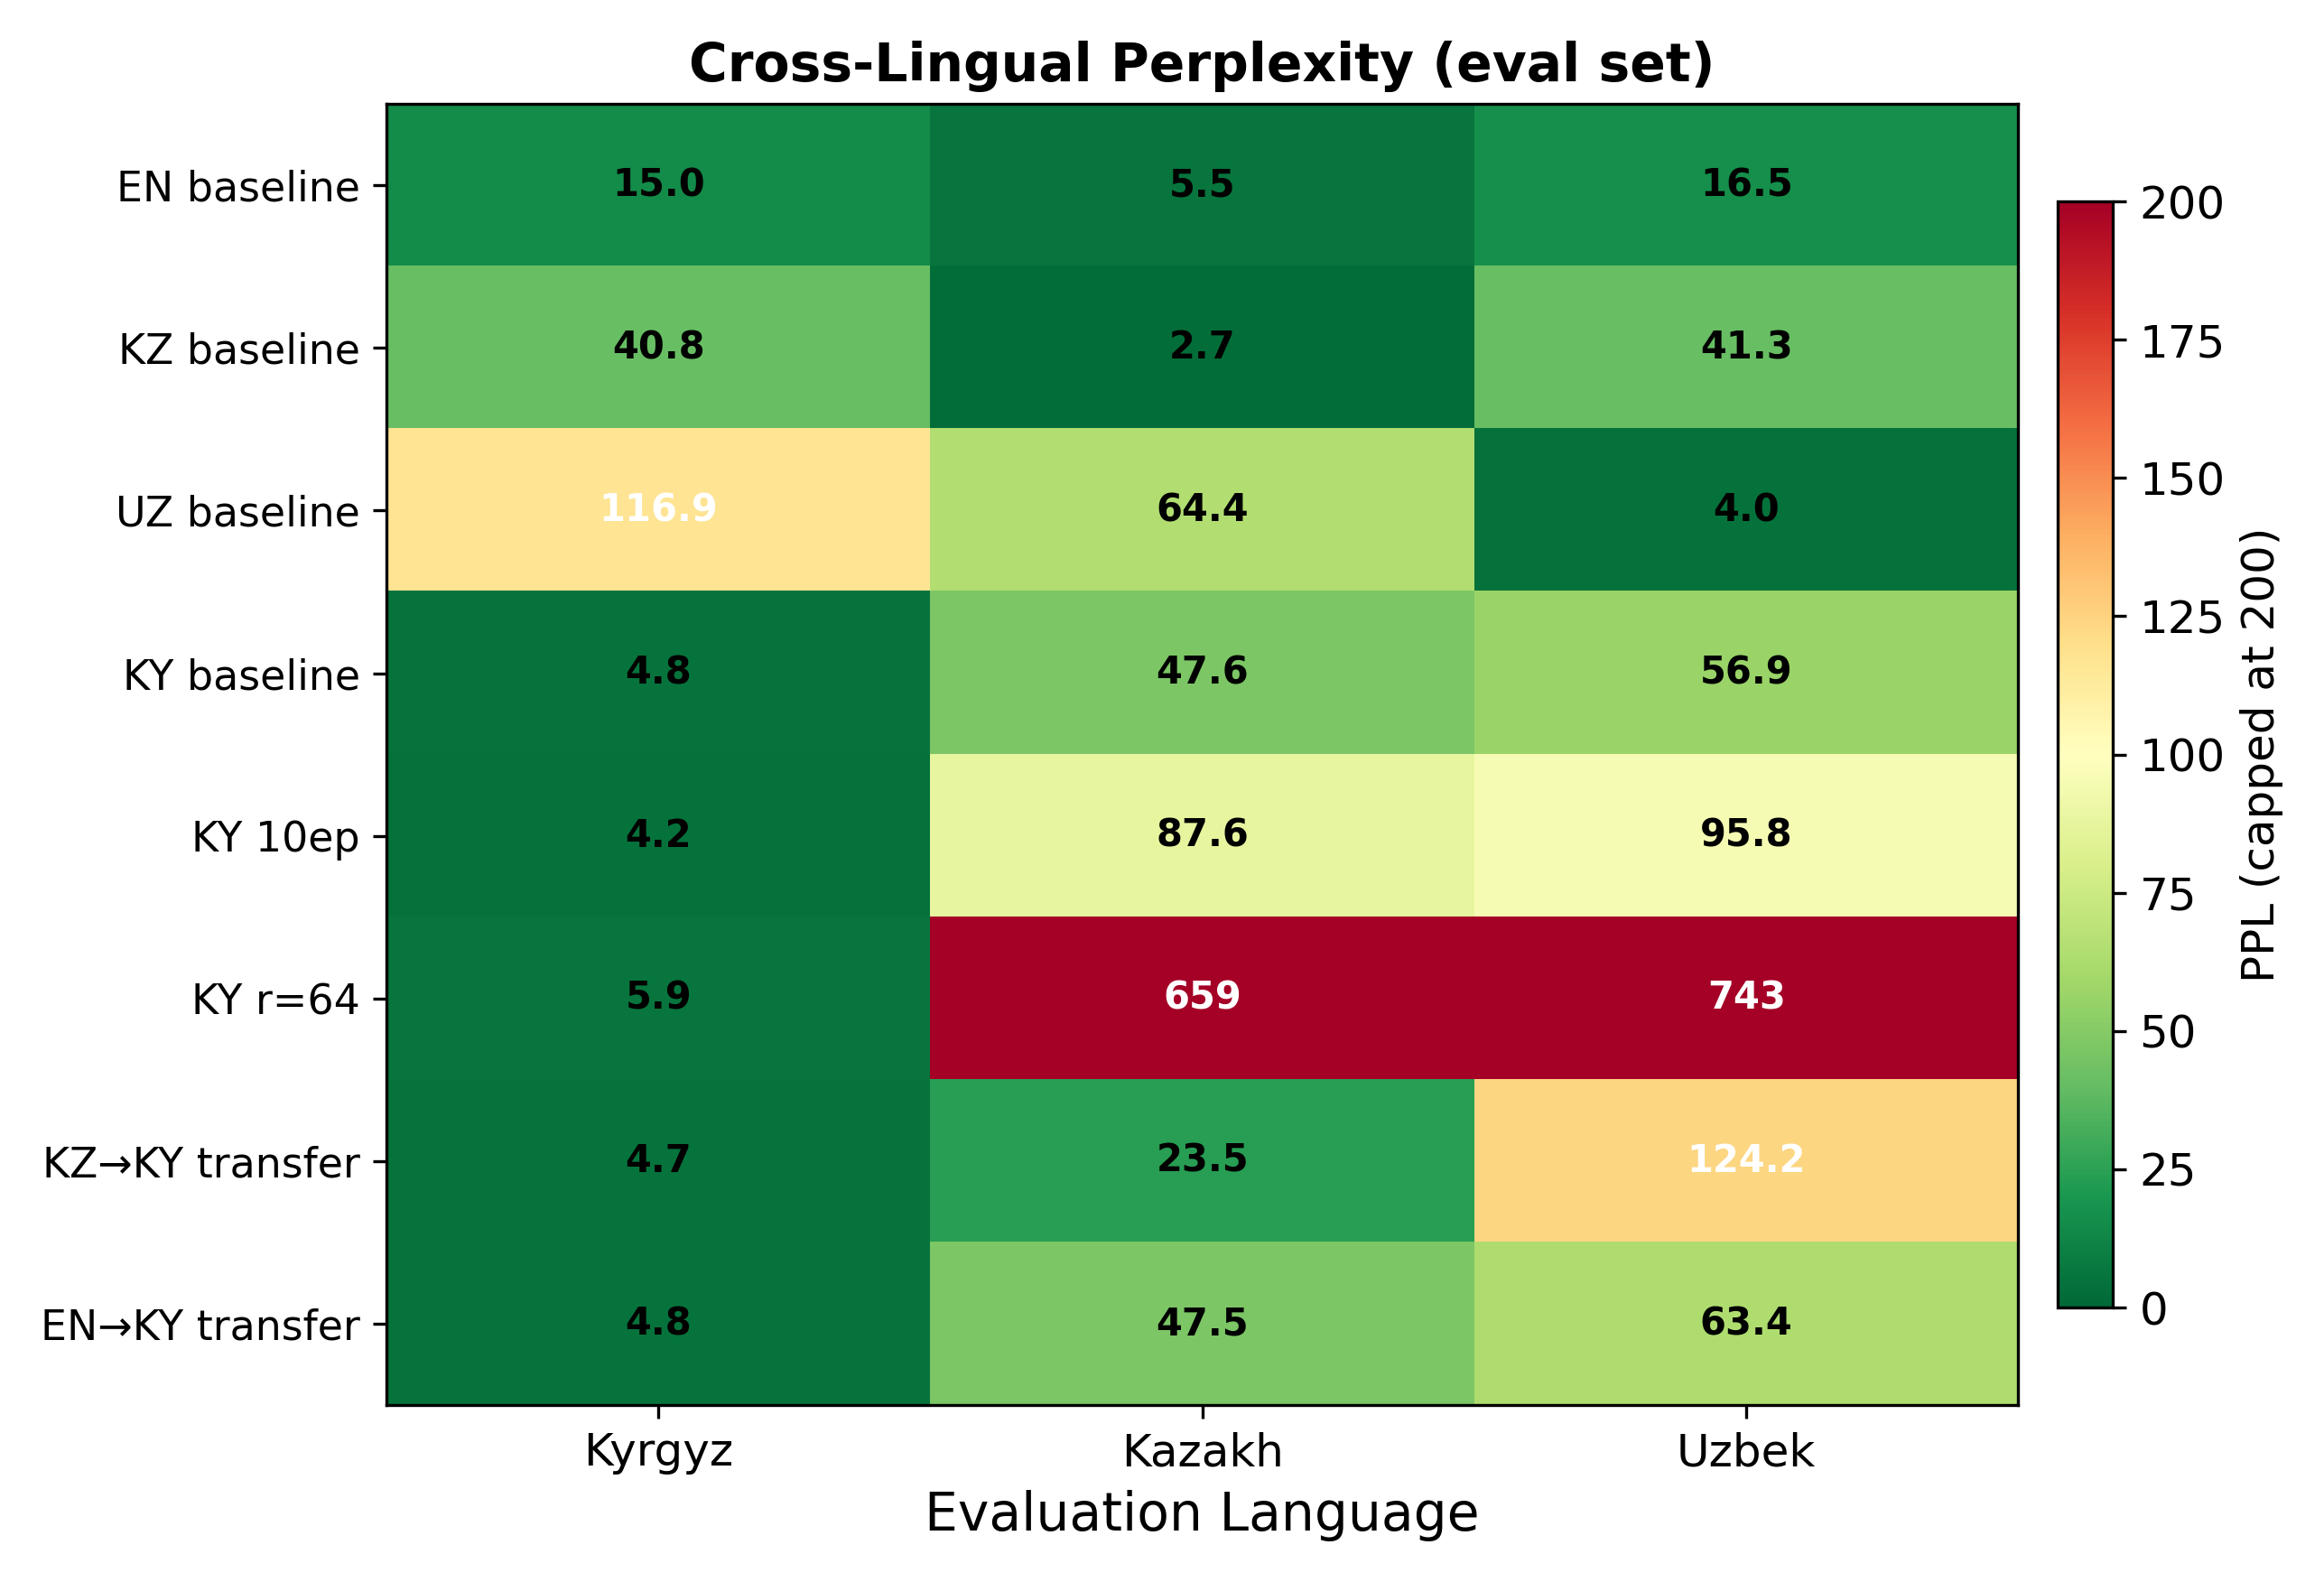
\includegraphics[width=0.75\textwidth]{../figures/fig4_cross_ppl.png}
    \caption{Cross-lingual perplexity heatmap. Darker cells indicate higher perplexity (more forgetting). Color is clipped at $200$: cells with PPL $> 200$ (notably E5's KZ at $659$ and UZ at $743$) render as the darkest red but retain their numeric annotation, so the numeric values remain readable while the color palette does not flatten the lower-PPL contrasts elsewhere in the matrix. The $r{=}64$ row is clearly pathological, while the KZ$\rightarrow$KY transfer row shows the most balanced profile.}
    \label{fig:cross_ppl}
\end{figure*}

\subsection{Spectral Energy is Not a Reliable Collapse Diagnostic}
\label{sec:spectral}

Our central finding is that the spectral energy threshold of 0.7 proposed by \citet{biderman2024lora} is \textbf{never reached} in any of our experiments, including those exhibiting severe functional degradation. \Cref{fig:svd_dynamics} shows the evolution of mean and maximum SE across training steps for representative experiments.

\begin{figure*}[t]
    \centering
    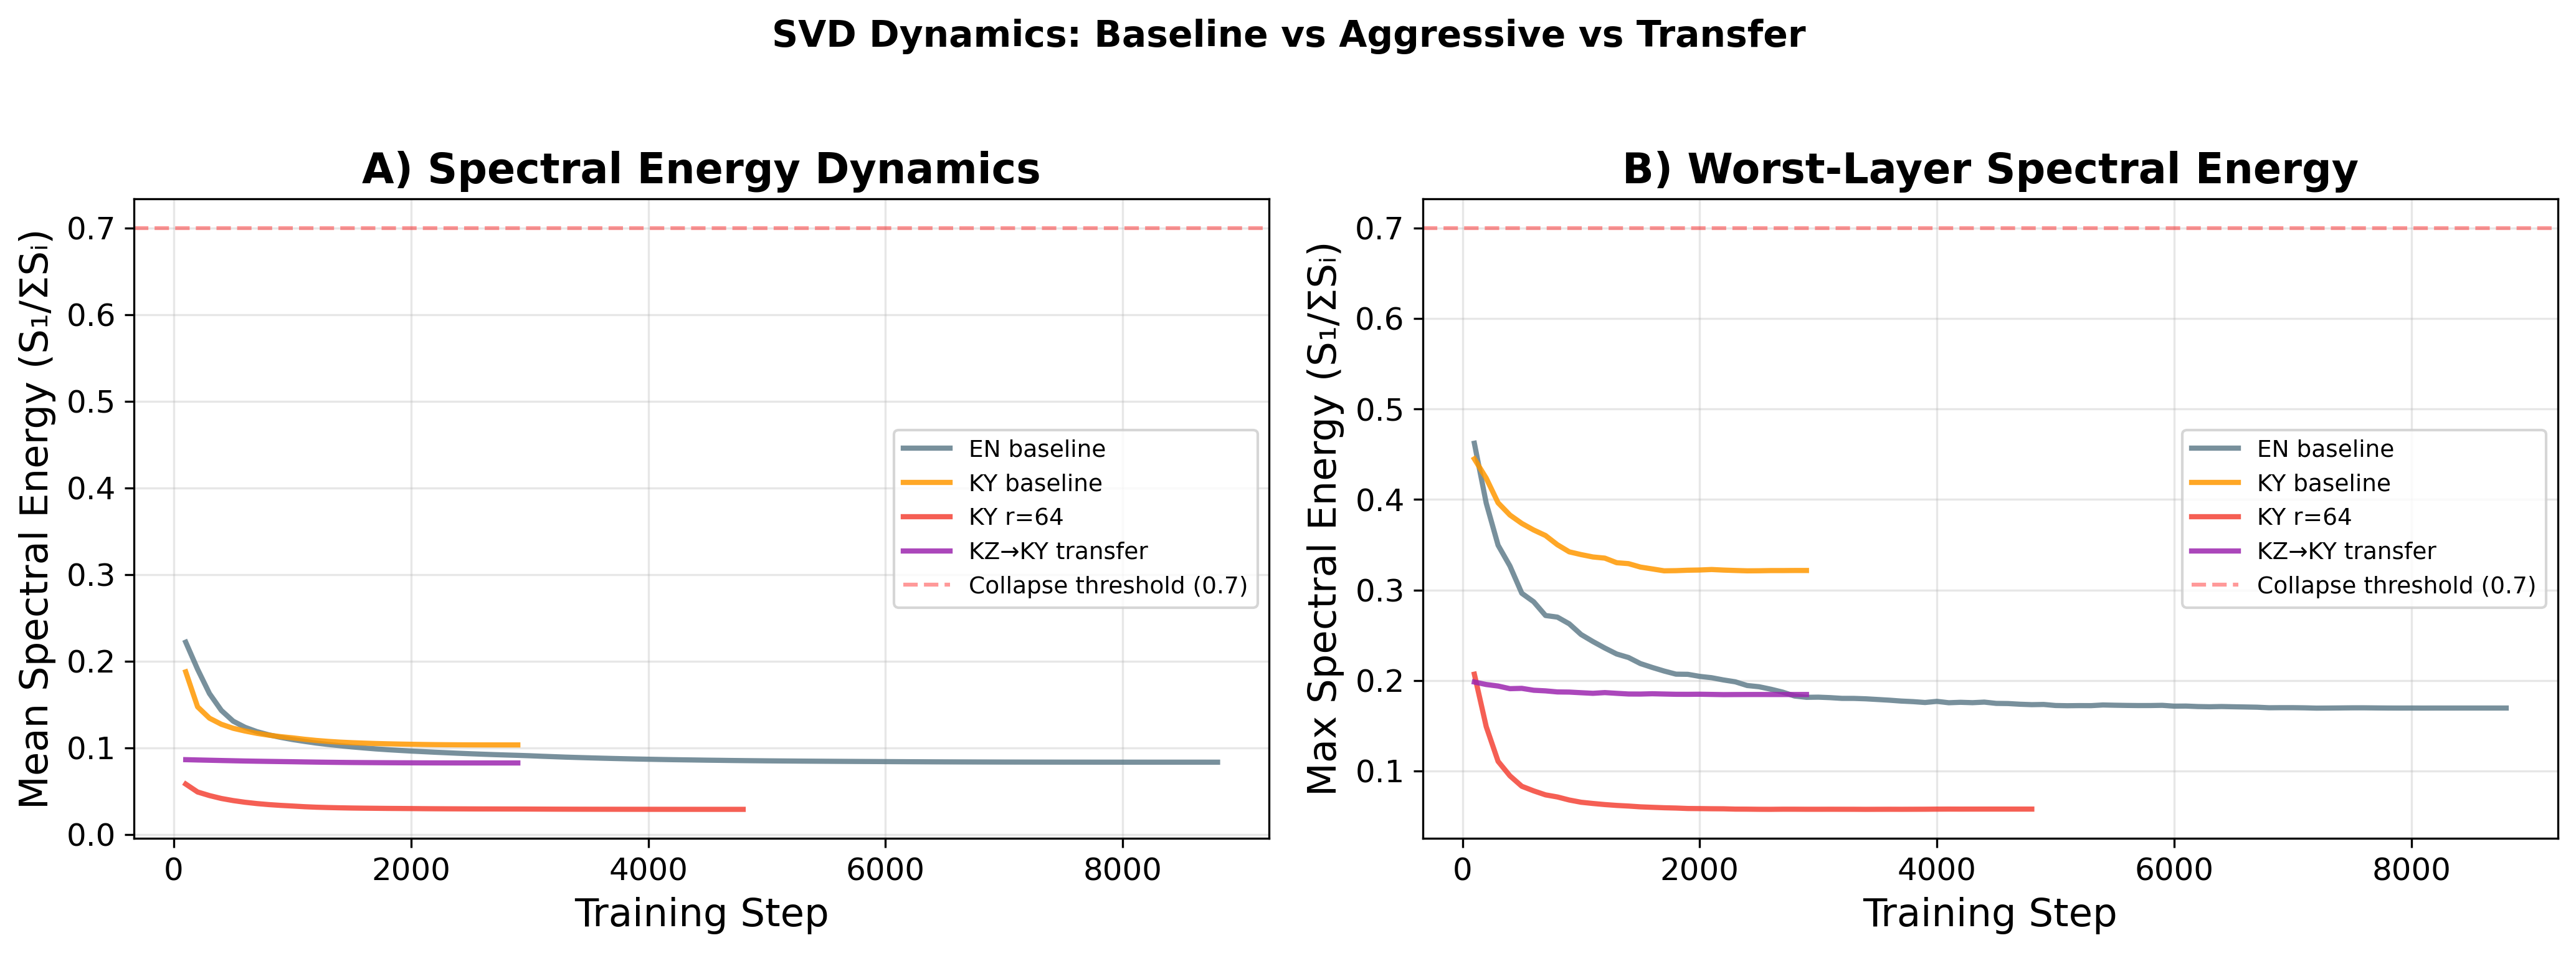
\includegraphics[width=\textwidth]{../figures/fig2_svd_dynamics.png}
    \caption{Spectral energy dynamics during training. Top: mean SE across all layers. Bottom: maximum SE across layers. No experiment approaches the proposed 0.7 threshold. The $r{=}64$ configuration shows \emph{decreasing} SE despite suffering the worst functional degradation.}
    \label{fig:svd_dynamics}
\end{figure*}

The KY baseline ($r{=}16$) shows maximum SE peaking near $0.44$ in the first $\sim 100$ steps and then \emph{decreasing} to $\sim 0.32$ at the final checkpoint, well below the 0.7 threshold throughout. Both $r{=}64$ configurations---the collapsed E5 and the healthy-adapting E5b---show the same qualitative pattern but at much smaller values, ending at final mean SE $\sim 0.03$ and final max SE $\sim 0.06$--$0.11$ (well below the threshold). The fact that E5 and E5b end with near-identical spectral profiles yet completely different functional behavior (NER F1~$= 0$ vs.\ 0.146; TUMLU 23\% vs.\ 33\%) is a direct falsification of SE as a diagnostic in our setting: SE is a \emph{shape} metric that cannot distinguish the two regimes. As training progresses, all singular values grow, but the growth is distributed across multiple directions, causing the relative contribution of $\sigma_1$ to decrease---regardless of whether the adapter has collapsed functionally.

The effective rank tells a complementary story: for both $r{=}64$ configurations, effective rank \emph{increases} from initialization, indicating that the adapter is utilizing more of its available capacity. Under standard interpretations, increasing effective rank signals healthy training dynamics. Yet the high-LR E5 configuration suffers complete NER failure and catastrophic cross-lingual forgetting despite this ``healthy'' trajectory, while the controlled-LR E5b does not---again showing that the spectral trajectory alone cannot distinguish the two.

\Cref{fig:layer_heatmap} shows the layer-wise SE distribution at the final checkpoint, confirming that no individual layer approaches the collapse threshold.

\begin{figure*}[t]
    \centering
    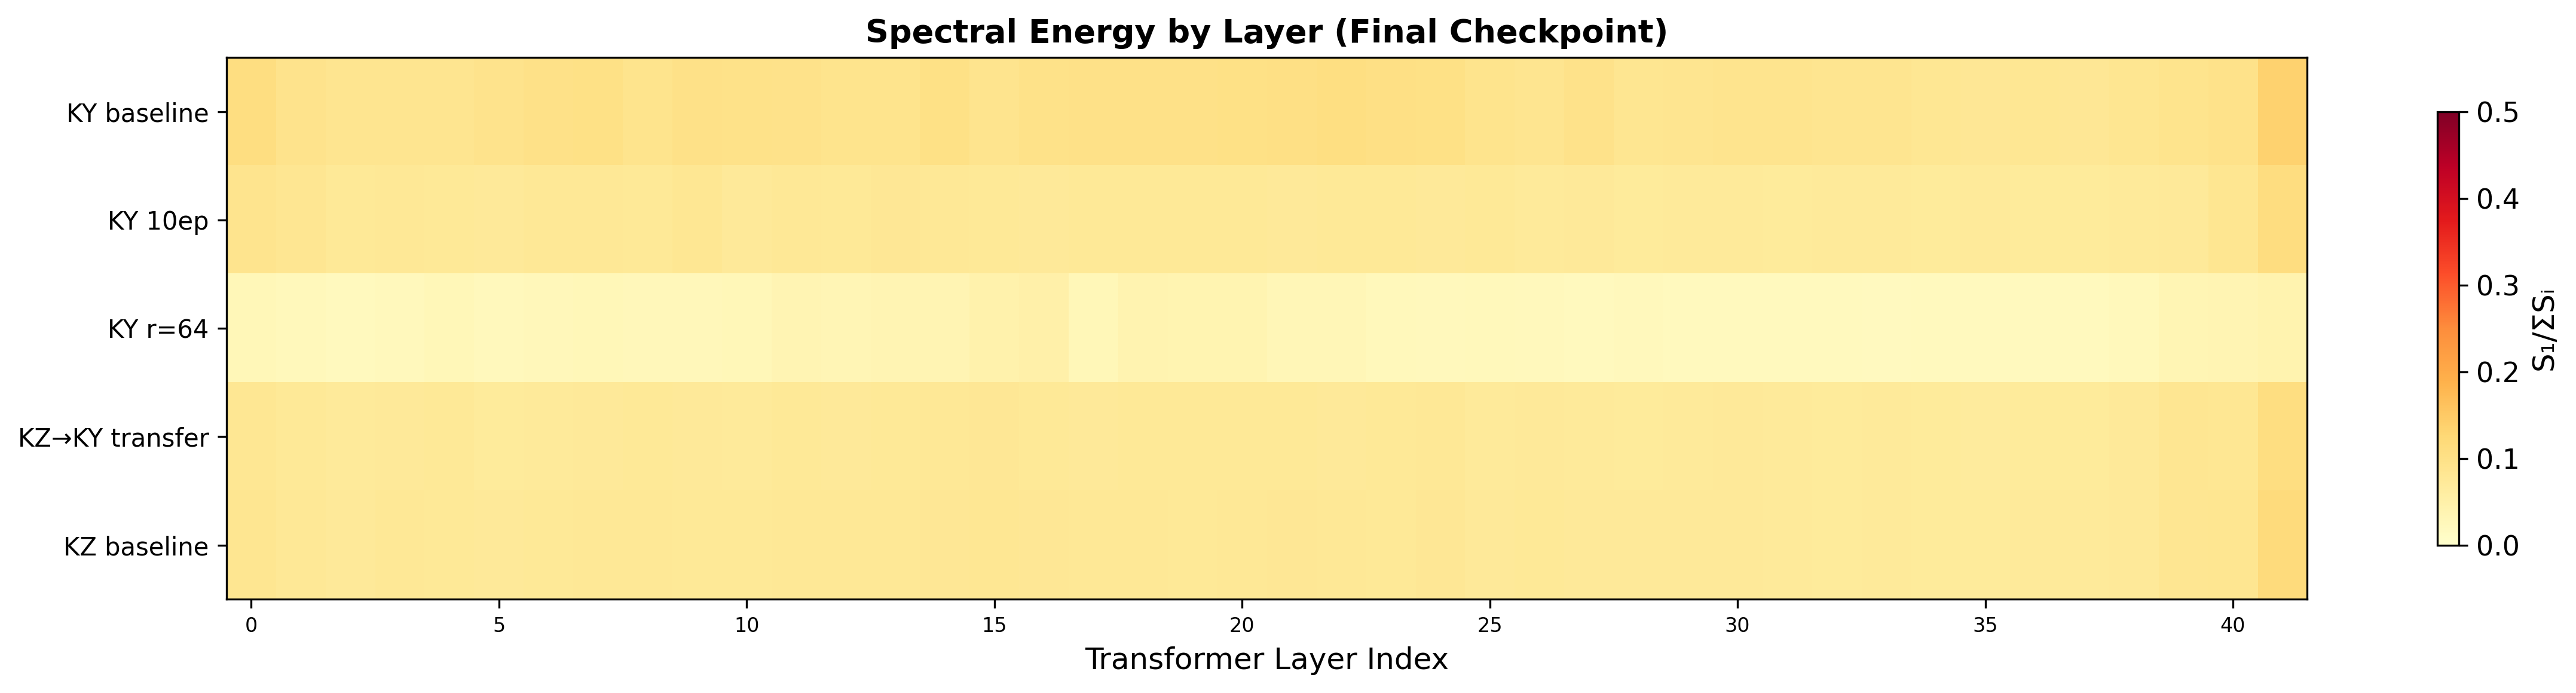
\includegraphics[width=\textwidth]{../figures/fig3_layer_heatmap.png}
    \caption{Layer-wise spectral energy at the final training checkpoint. Each row is an experiment; each column is a transformer layer. No layer in any experiment exceeds the 0.7 threshold.}
    \label{fig:layer_heatmap}
\end{figure*}

\textbf{Quantization is not the cause (BF16 control, C3).} A reviewer-prompted concern was that 4-bit NF4 quantization might itself suppress spectral growth and account for the sub-threshold SE. We address this with a dedicated full-precision (bfloat16, no quantization) replication of the KY baseline (E3 setup, $r{=}16$, $\text{lr}{=}2{\times}10^{-4}$, 3 epochs) on a cloud A100. The result confirms, rather than weakens, the SE finding: BF16 and 4-bit produce essentially indistinguishable SE behaviour. In BF16 the final-checkpoint max SE is $0.32$ and final mean SE is $0.10$, matching 4-bit E3 within seed variance ($0.33 \pm 0.01$ and $0.10$ across two seeds; \Cref{tab:bf16}); the in-training peak max SE is also comparable ($0.47$ in BF16 vs.\ $0.45 \pm 0.02$ in 4-bit E3 across seeds). Frobenius norm growth at the same point is $8.6\times$ in BF16 versus $8.4\times$ in E3---indistinguishable. Cross-lingual perplexity, NER F1, log-likelihood span typing, and TUMLU accuracy are all within $\pm$1 standard deviation of the seed-level variance we observe for E3 across two seeds (\Cref{app:seed_variance,tab:bf16}). Quantization granularity therefore does not materially alter spectral or downstream behaviour in our setting; the SE-threshold falsification carries over from 4-bit to full precision.

\textbf{H1 is not supported in our setting:} spectral energy below the proposed threshold does \emph{not} guarantee healthy training, and SE can decrease during training that leads to functional collapse. We note that our experiments use 4-bit NF4 quantization, which may itself suppress singular value growth relative to the full-precision setting of \citet{biderman2024lora}; our findings therefore challenge the generality of the SE threshold rather than refuting it unconditionally. The SE metric fundamentally measures the \emph{shape} of the singular value distribution while ignoring its \emph{scale}---a critical limitation when diagnosing pathological training regimes in quantized, low-resource settings.

\subsection{Frobenius Norm: The Missing Diagnostic}
\label{sec:frobenius}

If spectral energy fails as a diagnostic, what about scale-aware alternatives? We examine the \textbf{Frobenius norm growth ratio} of the $\texttt{lora\_B}$ matrices, which captures the magnitude of weight perturbations that SE discards. While Frobenius growth provides better separation than SE in some regimes, our cross-language and cross-rank analysis shows it is also \emph{not} a universal diagnostic.

\begin{table}[t]
\centering
\small
\begin{tabular}{lccc}
\toprule
\textbf{Experiment} & $\|\mathbf{B}\|_F^{\text{init}}$ & $\|\mathbf{B}\|_F^{\text{final}}$ & \textbf{Growth} \\
\midrule
KZ$\rightarrow$KY Transfer (E6, related) & 3.043 & 3.436 & 1.13$\times$ \\
EN$\rightarrow$KY Transfer (E6b, cross-family) & 0.653 & 2.023 & 3.10$\times$ \\
KY Baseline $r{=}16$ & 0.227 & 1.899 & 8.36$\times$ \\
EN Control $r{=}16$ & 0.092 & 3.076 & 33.4$\times$ \\
KY BF16 $r{=}16$ (C3) & 0.218 & 1.880 & 8.6$\times$ \\
KZ Baseline $r{=}16$ & 0.081 & 3.107 & 38.5$\times$ \\
KY $r{=}64$ lr $5{\times}10^{-4}$, 5ep (E5) & 0.566 & 8.859 & 15.6$\times$ \\
KY $r{=}64$ lr $2{\times}10^{-4}$, 5ep (E5b) & 0.247 & 4.486 & 18.2$\times$ \\
KY $r{=}64$ lr $2{\times}10^{-4}$, 3ep (E5c) & 0.388 & 3.385 & 8.7$\times$ \\
KY $r{=}64$ $\alpha{=}32$ 3ep (C5, matched-$\alpha$) & 0.456 & 3.900 & 8.55$\times$ \\
Diverged $r{=}64$ & --- & --- & explodes \\
\bottomrule
\end{tabular}
\caption{Frobenius norm growth ratios for $\texttt{lora\_B}$ matrices. ``Init'' is the first SVD-log measurement (training step 100), not the literal loaded checkpoint, because we log spectra every 100 steps. For E6 (KZ$\rightarrow$KY) the step-100 norm stays close to the loaded KZ-final norm ($3.04$ vs.\ $3.11$), indicating that the warm-started adapter barely moves during the first 100 KY steps. For E6b (EN$\rightarrow$KY) the step-100 norm drops sharply to $0.65$ from the loaded EN-final norm of $3.08$, consistent with the EN-init directions being misaligned with KY gradients and partially zeroed-out before the adapter is rebuilt. EN control and KZ baseline show comparable growth ($\sim$33--38$\times$), yet EN produces minimal cross-lingual forgetting (KZ PPL 5.54) while KY baseline with only 8$\times$ growth causes severe forgetting (KZ PPL 47.58). This demonstrates that norm growth alone is insufficient as a universal diagnostic. Note also that E5 and E5b exhibit comparable Frobenius growth (15.6$\times$ vs.\ 18.2$\times$), yet only E5 suffers NER parse failure and near-random TUMLU. The cross-family transfer E6b shows intermediate growth ($3.10\times$), between related-language warm-start ($1.13\times$) and random init ($8.36\times$).}
\label{tab:frobenius}
\end{table}

\Cref{tab:frobenius} and \Cref{fig:frobenius} reveal a nuanced picture. The KZ$\rightarrow$KY transfer exhibits only $+13\%$ Frobenius norm growth, while the KY baseline shows $\sim$8$\times$ growth and the pathological $r{=}64$ configuration shows 15--38$\times$ growth. However, the EN control experiment complicates this gradient: despite $\sim$33$\times$ norm growth---comparable to the KZ baseline (38$\times$)---EN training causes minimal cross-lingual forgetting (KZ PPL $5.52 \pm 0.02$ across 2 seeds vs.\ $\sim$48 for the KY baseline with only 8$\times$ growth). This EN-vs-Turkic dissociation is consistent across two seeds (E8 Frobenius growth $33.39\times$ at seed~42 and $33.17\times$ at seed~123; see \Cref{app:seed_variance}). It reveals that Frobenius norm growth is a reliable diagnostic \emph{within} a language category (underrepresented vs.\ well-represented) but not \emph{across} categories: the same magnitude of weight perturbation has qualitatively different effects depending on how well the target language is represented in the pretrained model.

\begin{figure*}[t]
    \centering
    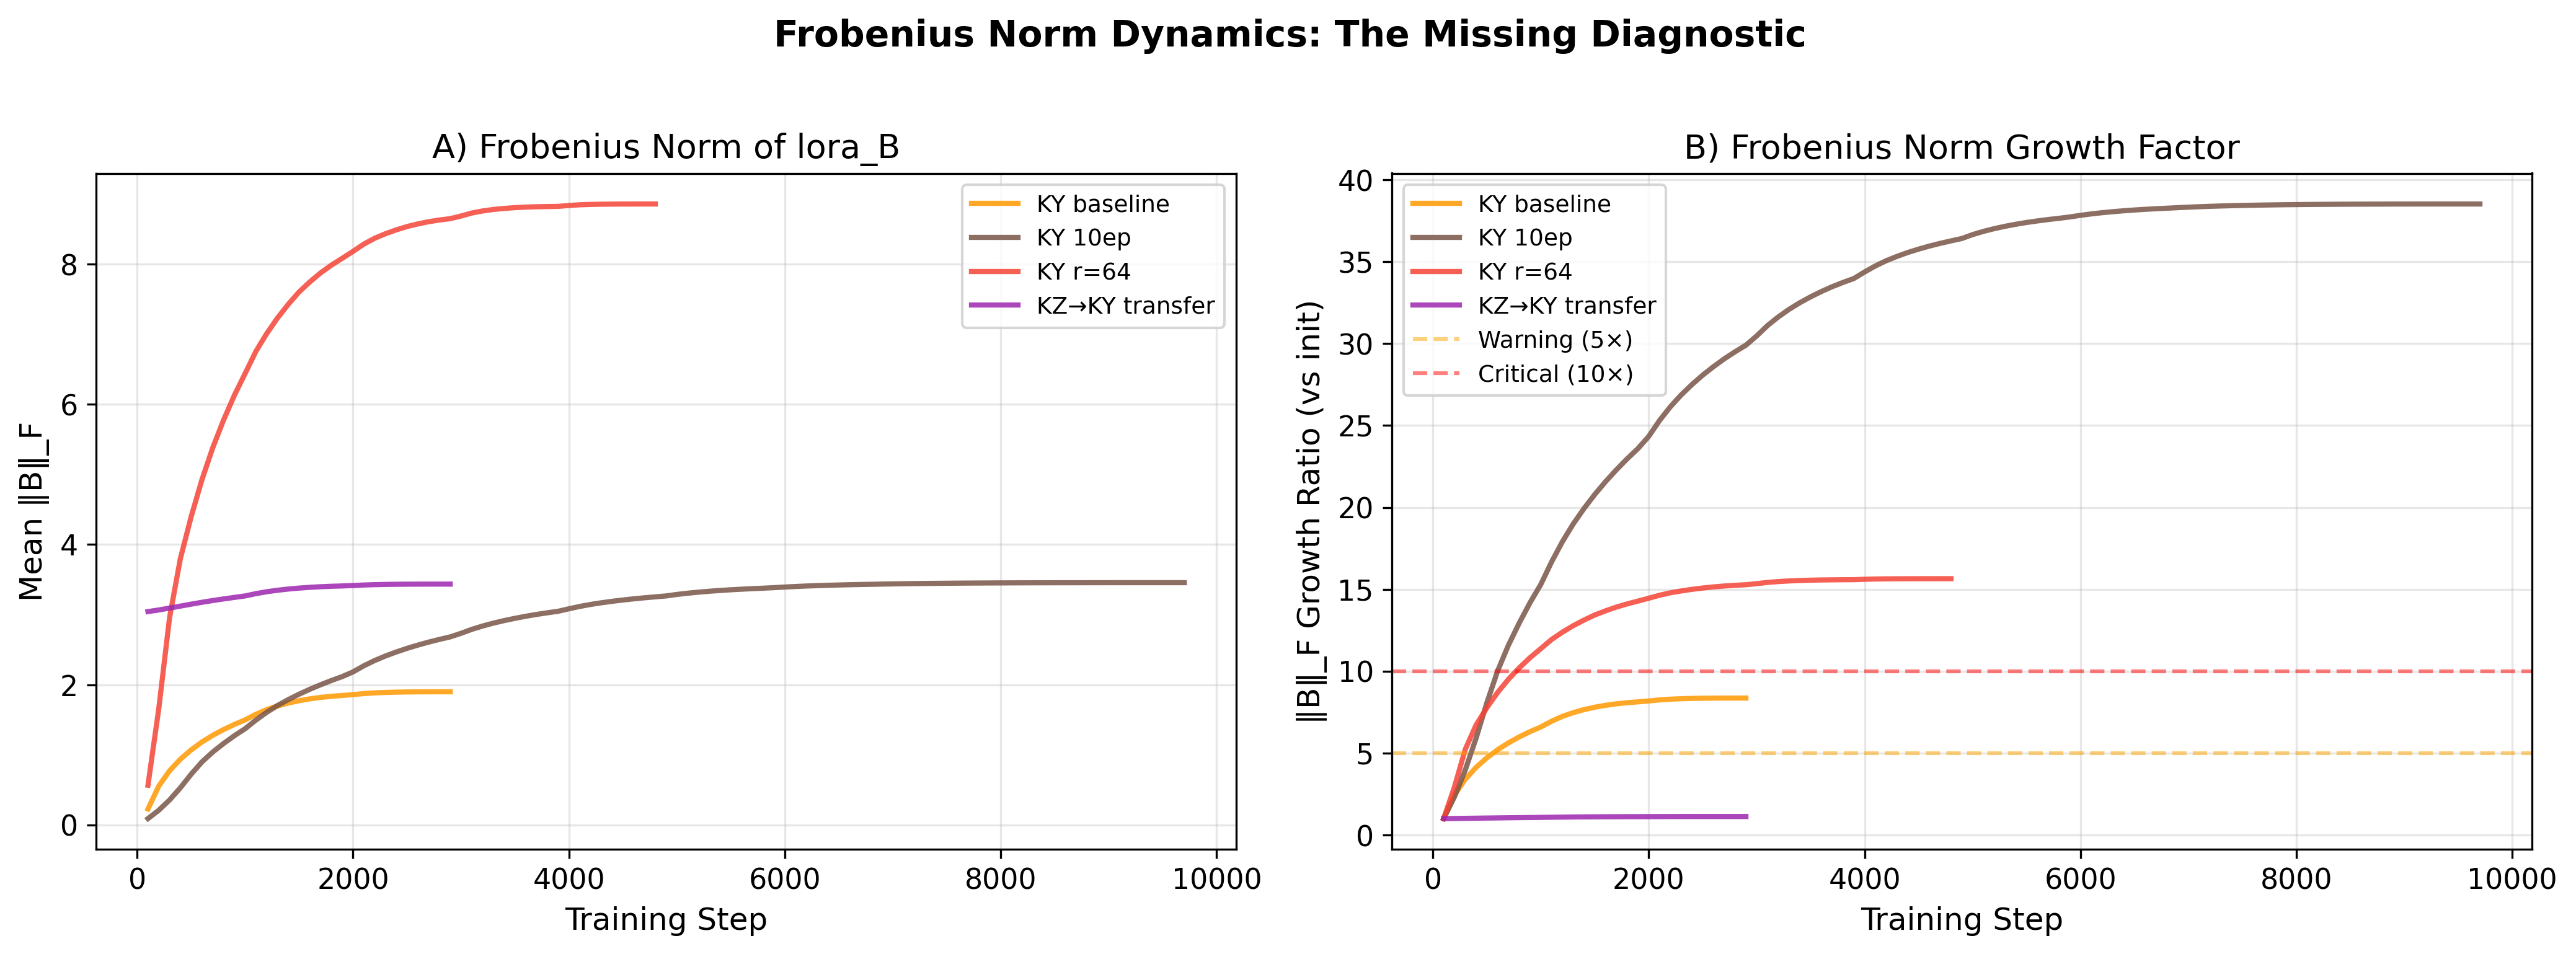
\includegraphics[width=\textwidth]{../figures/fig6_frobenius_dynamics.png}
    \caption{Frobenius norm dynamics of $\texttt{lora\_B}$ matrices during training. The $r{=}64$ configuration shows dramatically larger norm growth compared to $r{=}16$ baselines. The related-language transfer (KZ$\rightarrow$KY) begins at the KZ baseline's final norm and shows minimal additional growth ($+13\%$). The cross-family transfer (EN$\rightarrow$KY) begins at the EN baseline's final norm and shows intermediate growth ($3.1\times$), sitting geometrically between the related-language warm-start and direct training---supporting the "better initialization" interpretation of Section~\ref{sec:transfer}.}
    \label{fig:frobenius}
\end{figure*}

\Cref{fig:frobnorm_scatter} visualizes the relationship between Frobenius norm growth and cross-lingual PPL degradation. We do not perform a formal statistical test, as our sample size ($n{=}7$ Turkic experiments) is far too small for a meaningful rank-correlation test. Visually, within the Turkic experiments the trend is in the expected direction (more growth, more forgetting), but the EN control is a clear outlier ($33\times$ growth with minimal forgetting), indicating that norm growth alone is not sufficient to predict catastrophic forgetting. The Frobenius norm is a \emph{scale-aware} metric that captures the total magnitude of weight updates, but the \emph{direction} of those updates---whether they reinforce or disrupt pretrained representations---is the question we take up in \Cref{sec:directional}.

\begin{figure*}[t]
    \centering
    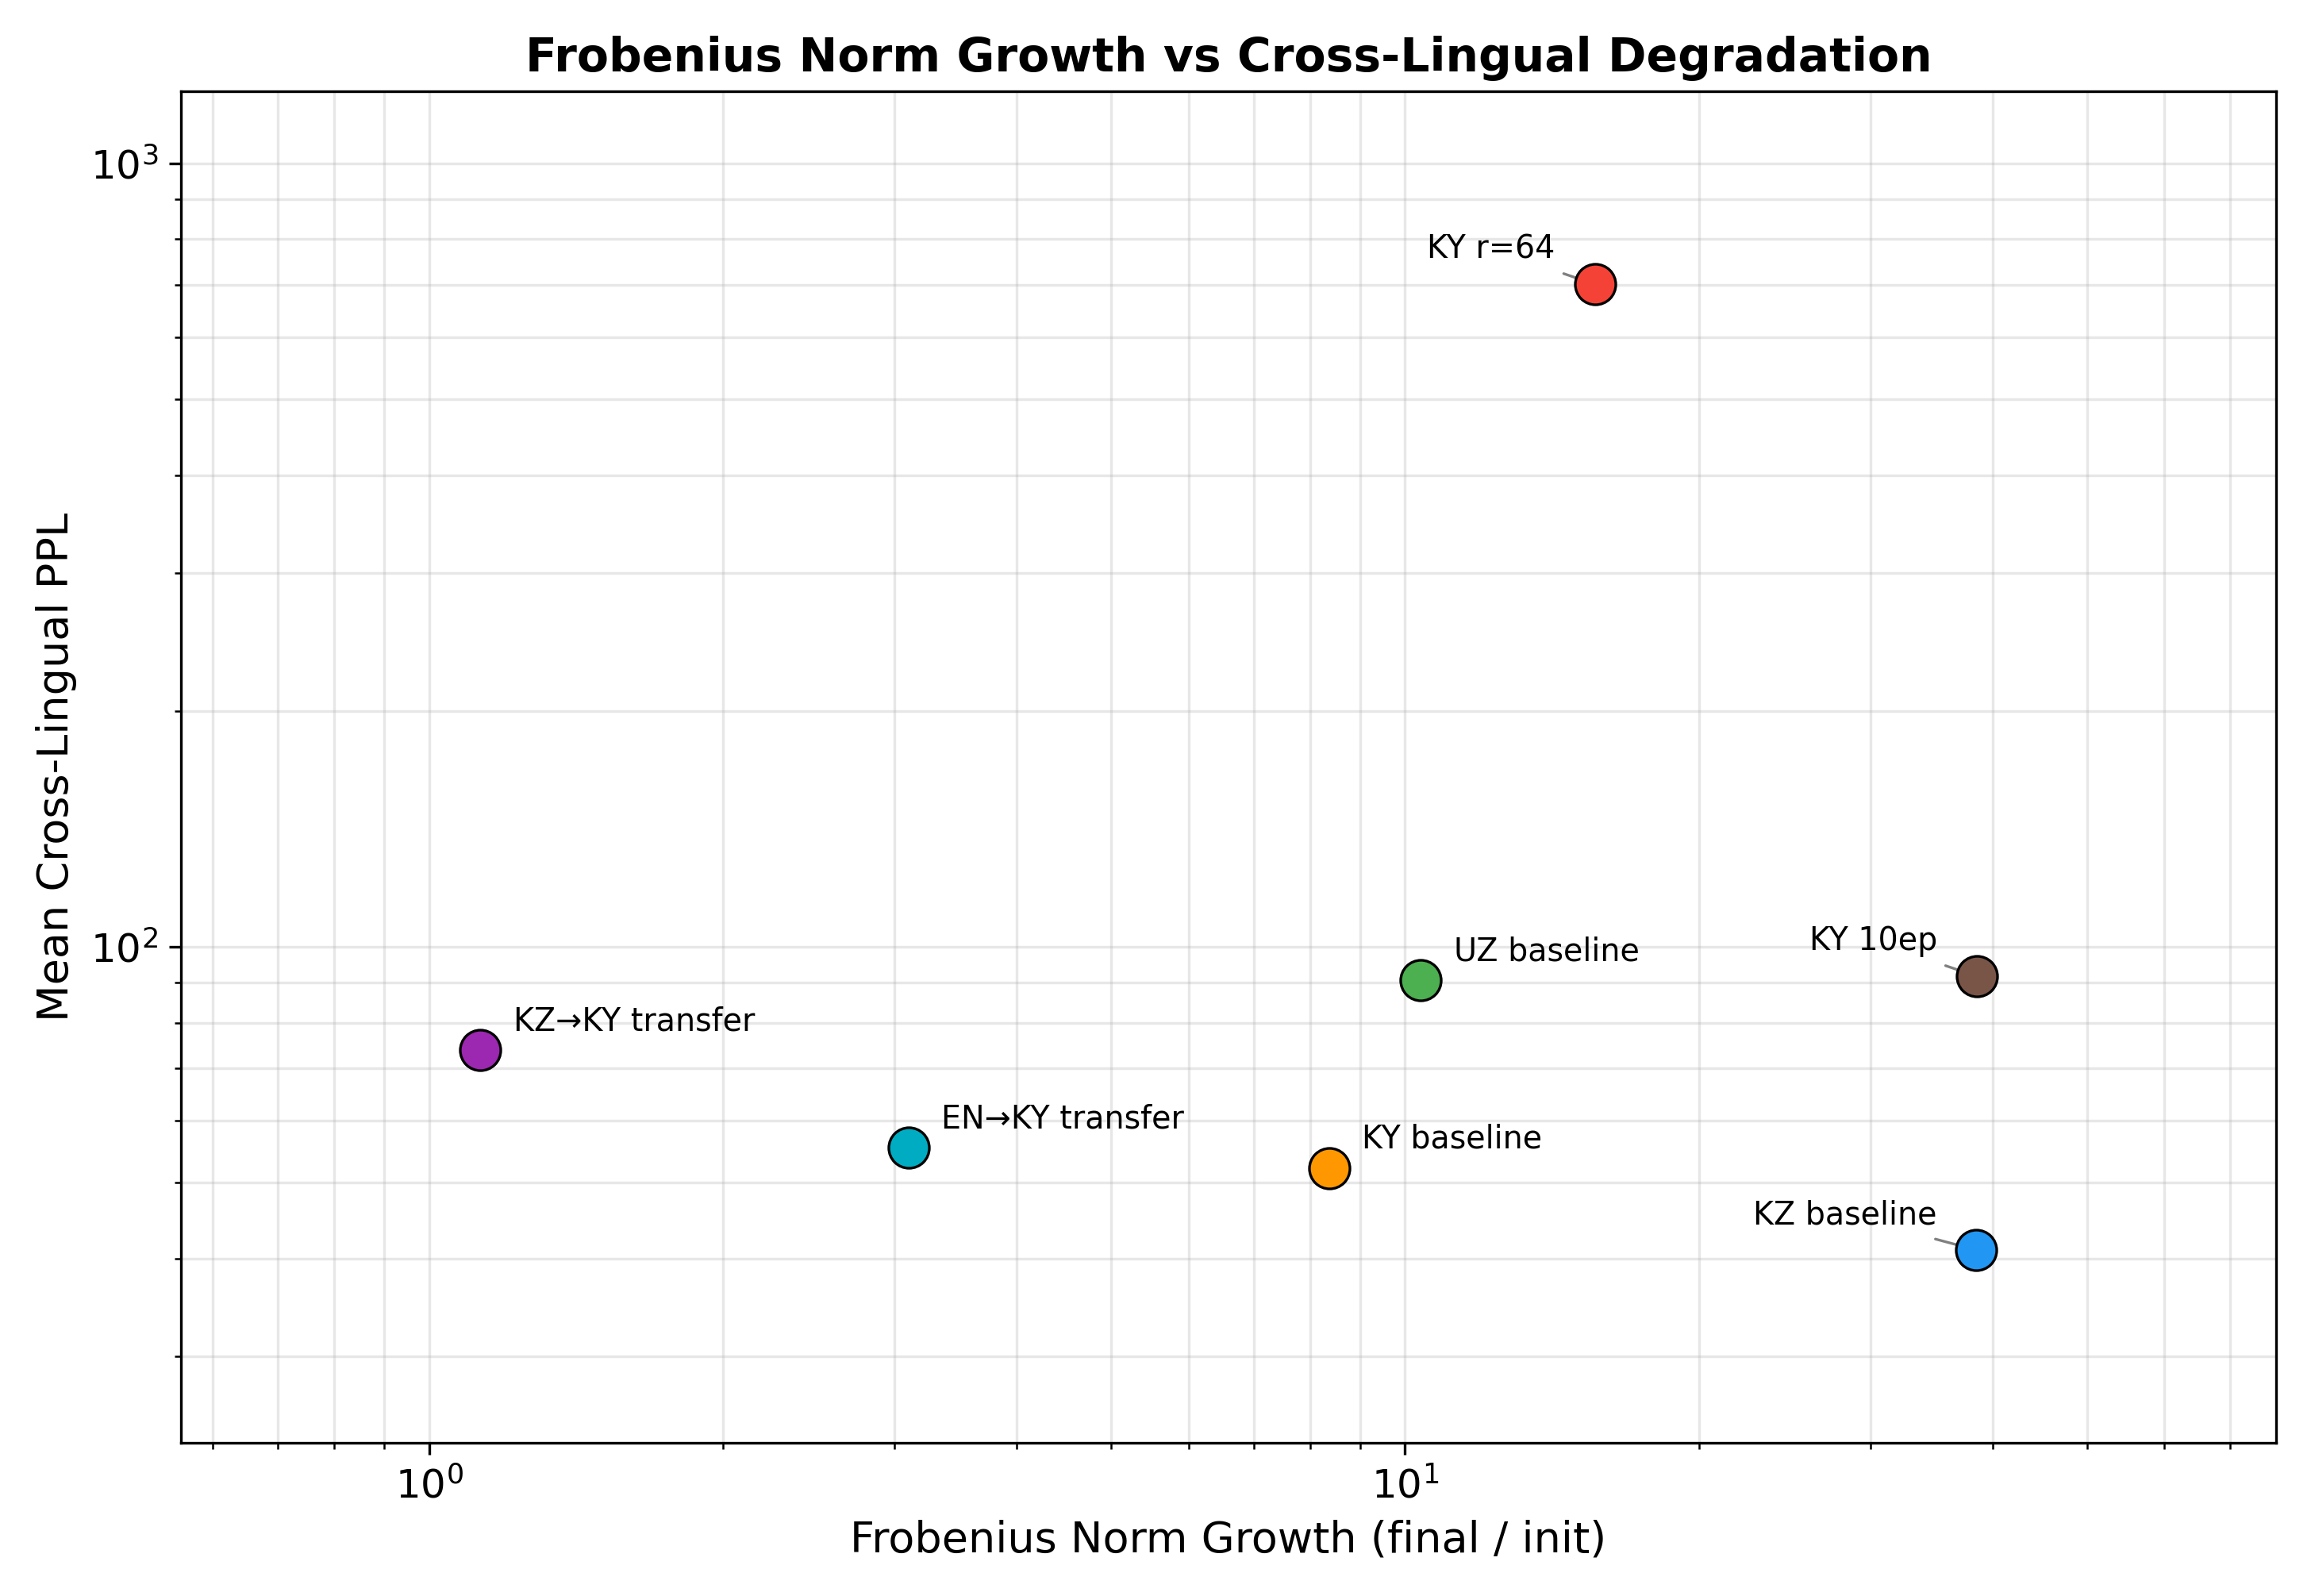
\includegraphics[width=0.75\textwidth]{../figures/fig9_frobnorm_vs_ppl.png}
    \caption{Frobenius norm growth ratio versus cross-lingual perplexity degradation. Larger norm growth is associated with more severe catastrophic forgetting within Turkic experiments, but the EN control sits at $33\times$ growth with minimal forgetting---norm growth alone is not sufficient to predict catastrophic forgetting.}
    \label{fig:frobnorm_scatter}
\end{figure*}

\subsection{Cross-Lingual Transfer}
\label{sec:transfer}

The KZ$\rightarrow$KY transfer experiment (E6) initializes LoRA adapters from the final Kazakh checkpoint (E1) before continuing training on Kyrgyz data. This simple sequential transfer yields substantial improvements across multiple metrics (\Cref{tab:transfer}).

\begin{table}[t]
\centering
\small
\begin{tabular}{lcc}
\toprule
\textbf{Metric} & \textbf{KY Baseline} & \textbf{KZ$\rightarrow$KY} \\
\midrule
PPL (KY) & 4.78 & 4.73 \\
PPL (KZ) & 47.58 & 23.49 \\
PPL (UZ) & 56.85 & 124.19 \\
NER F1 (KY) & 0.157 & 0.253 \\
NER F1 (KZ) & 0.190 & 0.130 \\
NER F1 (UZ) & 0.326 & 0.348 \\
TUMLU (KY) & 34.7\% & 33.7\% \\
TUMLU (KZ) & 30.2\% & 31.7\% \\
$\|B\|_F$ growth & 8.36$\times$ & 1.13$\times$ \\
\bottomrule
\end{tabular}
\caption{Comparison of direct Kyrgyz training (E3) and Kazakh$\rightarrow$Kyrgyz transfer (E6), reported at seed~$42$. Transfer's most robust effect is KZ retention (PPL $23.49$ vs.\ $47.58$; $23.5 \pm 0.1$ vs.\ $50.0 \pm 2.4$ across two seeds---\Cref{app:seed_variance}). The single-seed KY NER F1 improvement of $+61\%$ ($0.253$ vs.\ $0.157$) is \emph{not} robust to reseeding (seed~$123$: $0.179$ vs.\ $0.182$); we therefore characterize transfer as a retention mechanism rather than a target-NER improvement. UZ PPL increases under transfer ($124.19$ vs.\ $56.85$), suggesting the benefit is specific to closely related Kipchak languages.}
\label{tab:transfer}
\end{table}

The most visible improvement at seed~$42$ is Kyrgyz NER F1: 0.253 versus 0.157, a relative improvement of $+61\%$. However, a second seed ($123$) gives 0.179 vs.\ 0.182 for the same comparison---the NER-F1 advantage is not robust across seeds (see \Cref{app:seed_variance}). Target-language perplexity is essentially identical under both seeds ($4.73$--$4.78$ for E6 vs.\ $4.78$--$4.83$ for E3), indicating that the transfer does not sacrifice language modeling quality but also that it does not noticeably improve it. The one \emph{robust} transfer effect is Kazakh retention: KZ~PPL of $23.5 \pm 0.1$ versus $50.0 \pm 2.4$ across seeds, a $2\times$ improvement well outside seed variance, with KZ~TUMLU accuracy improving consistently ($31.7$--$32.6\%$ vs.\ $30.2$--$32.6\%$ at seed~$42$ and $123$ respectively).

Interestingly, even Uzbek NER F1 improves slightly under transfer (0.348 vs.\ 0.326), suggesting some positive transfer to the third Turkic language. However, Uzbek PPL degrades substantially (124.19 vs.\ 56.85, a 2.2$\times$ increase). This asymmetry has practical implications: sequential transfer between closely related languages (Kazakh and Kyrgyz are both Kipchak-branch, Cyrillic-script) can \emph{harm} more distant relatives (Uzbek, Karluk-branch, historically Latin-script). The adapter, having been optimized first for Kazakh then for Kyrgyz, specializes its weight updates in the Kipchak direction, displacing representations useful for Uzbek. Practitioners considering chain-of-transfer strategies should therefore monitor not only source-target retention but also collateral damage to typologically distant languages.

\textbf{Cross-family control (E6b): is any warm-start enough?} A natural concern with the above interpretation is that the KZ-retention effect in E6 could simply reflect "the adapter was trained on KZ first, so of course it remembers KZ"---in which case any warm-started adapter, even from an unrelated language, would yield similar retention of its own source. We address this with a cross-family control (E6b): same setup as E6 but warm-started from the English baseline (E8) instead of the Kazakh baseline (E1). If \emph{any} warm-start is sufficient, then EN$\rightarrow$KY should preserve the EN-baseline cross-lingual profile in the same way KZ$\rightarrow$KY preserves the KZ profile.

The data are inconsistent with this null. Across two seeds, EN$\rightarrow$KY converges to KZ PPL $48.8 \pm 1.4$ (seeds 42, 123: 47.46, 50.21)---within the seed-to-seed spread of direct training ($50.0 \pm 2.4$) and far above E6's $23.5 \pm 0.1$. The KY target and TUMLU values for EN$\rightarrow$KY also align with direct training rather than with E6.

\textbf{Frobenius growth interpolates between the two regimes:} KZ$\rightarrow$KY ($1.13\times$) $\ll$ EN$\rightarrow$KY ($3.10\times$) $\ll$ direct ($8.36\times$). The EN-initialized adapter requires $\sim 3\times$ more perturbation than the KZ-initialized one to reach KY competence, consistent with the EN baseline sitting geometrically further from a good KY solution. This provides direct quantitative support for the ``better initialization'' interpretation: the magnitude of additional weight perturbation is a smooth function of how close the warm-start sits to the target-language solution, not a binary "warm-start vs.\ cold-start" effect.

\textbf{The UZ side-effect is specific to Kipchak specialization.} E6 (KZ$\rightarrow$KY) shows substantially worse Uzbek perplexity ($124.19$) than direct KY training ($56.85$), a finding we had attributed to "Kipchak-direction specialization". E6b confirms this attribution: its UZ PPL is $63.42$, close to direct training and far below E6's degraded value. Sequentially passing through Kazakh therefore specifically displaces Uzbek-useful representations; initialization from an unrelated language (EN) does not.

\textbf{KY entity knowledge follows the same intermediate pattern.} Under log-likelihood TypeAcc (\Cref{tab:ner_loglik}), E6b sits between direct training and related-language transfer at $55.9 \pm 1.9\%$ across seeds (54.0, 57.7), consistent with cross-family initialization providing a partial---but smaller---entity-knowledge benefit than related-language transfer (E6: $62.2 \pm 2.7\%$). The TUMLU accuracy on KY for E6b is $36.0 \pm 0.1\%$ across seeds, slightly above both direct training ($36.1 \pm 1.4\%$) and E6 ($34.3 \pm 0.6\%$), but all three overlap within seed-to-seed spread.

\textbf{H2 is supported, and the cross-family control (E6b) clarifies its scope:} source-knowledge retention is specific to related-language initialization, not a generic checkpoint-reuse effect. The mechanism appears to be \emph{better initialization}: the KZ-trained adapter is already close to a good KY solution, so the additional perturbation needed is small ($+13\%$ Frobenius growth vs.\ $8.36\times$ for direct training), and this low-perturbation regime is what preserves the unrelated knowledge encoded in the checkpoint. An EN-initialized adapter, which sits further from a useful KY solution, requires a larger perturbation that effectively overwrites the source. Our sequential LoRA transfer differs from MAD-X \cite{pfeiffer2020madx}, which uses parallel language-specific adapters: we observe related-language initialization as a regularizing prior on the optimization trajectory, not as a structural disentanglement. The KZ$\rightarrow$KY checkpoint thus acts as a kind of geometric regularizer, and we next quantify this geometrically via the pairwise direction of adapter updates (\Cref{sec:directional}).

\subsection{Directional Geometry of LoRA Solutions}
\label{sec:directional}

Both spectral energy (\Cref{sec:spectral}) and Frobenius growth (\Cref{sec:frobenius}) are functions of the singular-value spectrum of $\Delta W{=}BA$, and both fail to separate $r{=}64$ collapse (E5) from $r{=}64$ healthy adaptation (E5c). A natural next probe is \emph{direction}: do the two configurations move the weights along the same axis in weight space, or along incompatible axes? We measure this by per-module Frobenius cosine between every pair of final adapters,
\begin{equation}
\cos_m(\Delta W_X, \Delta W_Y) \;=\; \frac{\langle B_X A_X,\; B_Y A_Y\rangle_F}{\|B_X A_X\|_F\,\|B_Y A_Y\|_F},
\end{equation}
computed without materializing the $\text{out}\times\text{in}$ product via the identity $\langle B_1 A_1, B_2 A_2\rangle_F = \mathrm{tr}(A_1^{\top} B_1^{\top} B_2 A_2)$. We report the mean and median of $\cos_m$ over the $42\times 7 = 294$ LoRA-equipped projections in Gemma-2-9B.

The 22-pair sweep in \Cref{tab:pairwise_cos} and \Cref{fig:pairwise_cos} reveals a sharp bimodal structure that none of the spectral or Frobenius diagnostics surface.

\begin{figure*}[t]
    \centering
    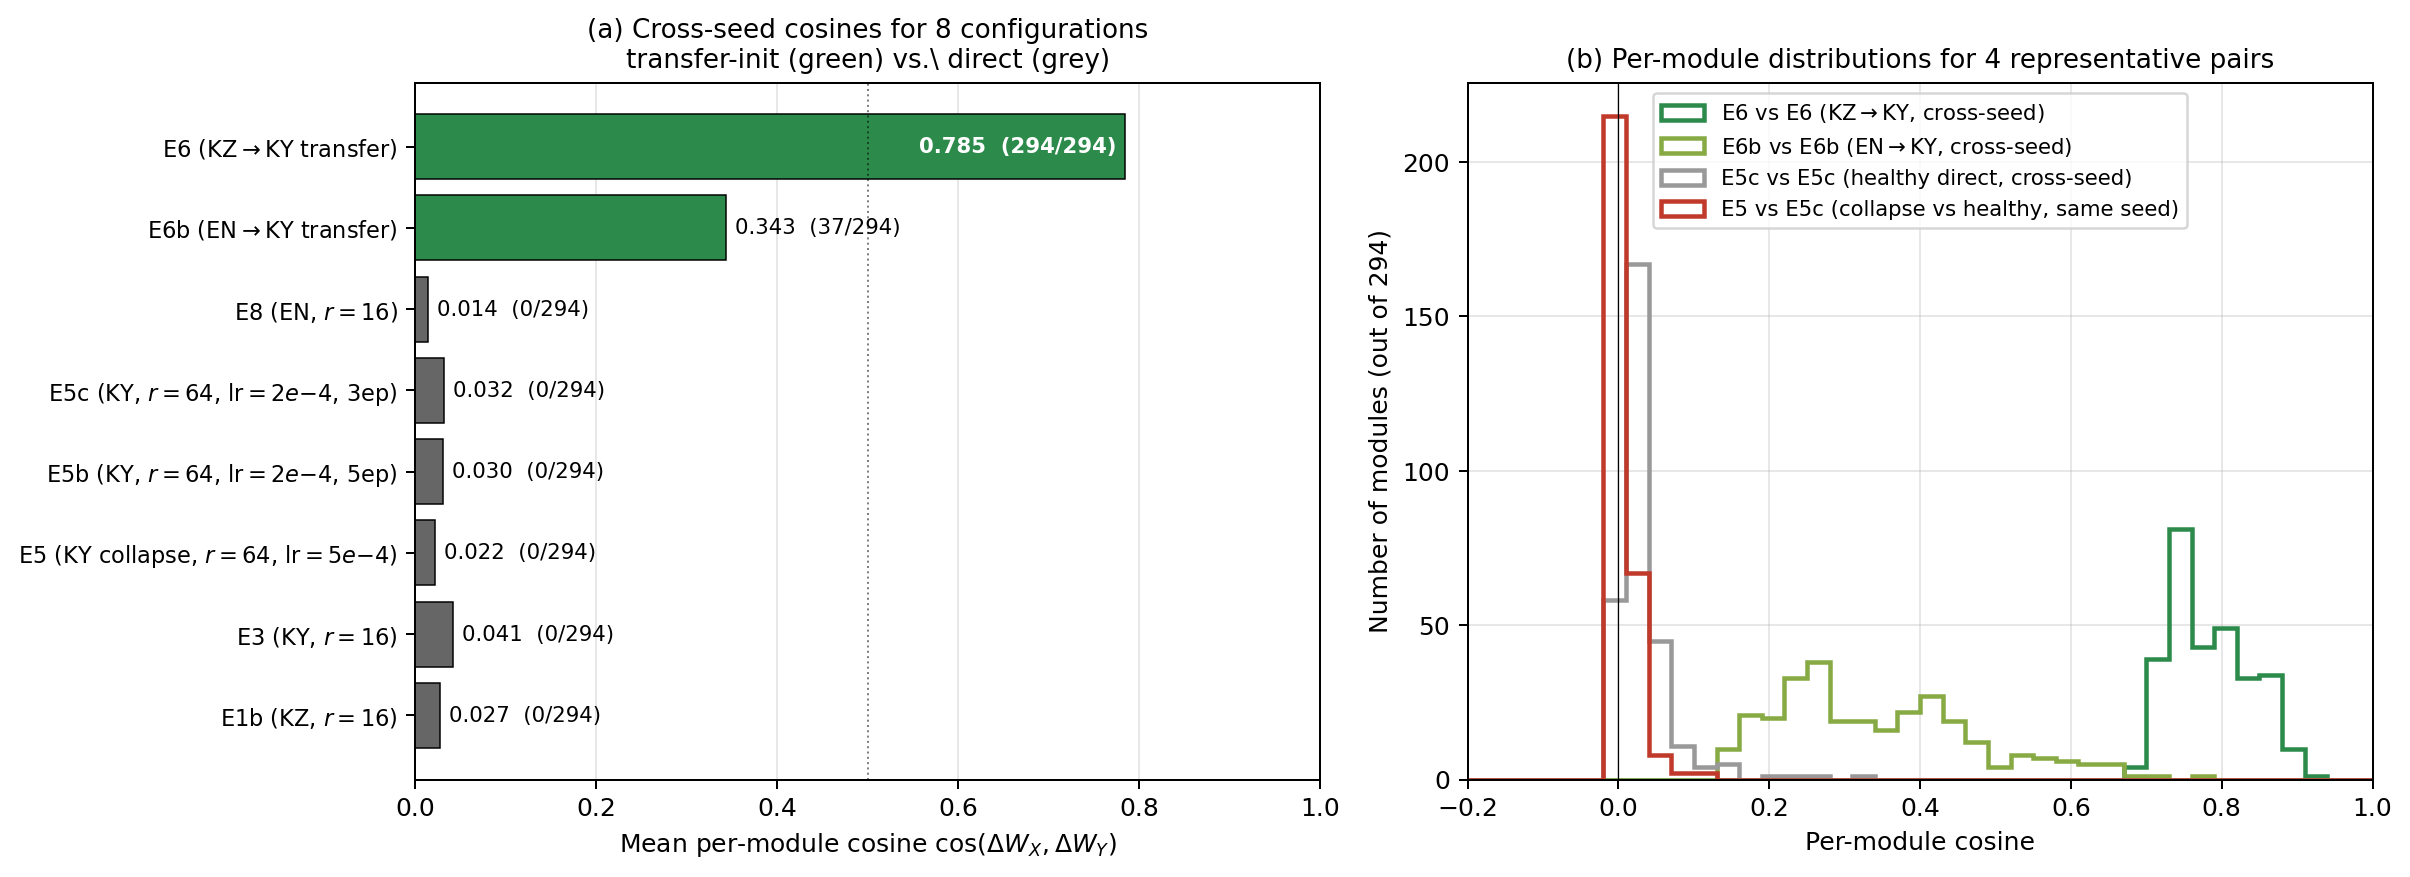
\includegraphics[width=\textwidth]{../figures/fig10_pairwise_cosine.png}
    \caption{Per-module Frobenius cosine between LoRA $\Delta W{=}BA$ matrices.
    \textbf{(a)} Cross-seed cosines for the eight seed-replicated configurations. Six direct-from-base configurations (grey: E1b, E3, E5, E5b, E5c, E8) cluster at mean cosine $0.01$--$0.04$ with $0/294$ modules above $0.5$; the two transfer-initialised configurations (green: E6, E6b) stand apart at $0.785$ and $0.343$ with $294/294$ and $37/294$ modules above $0.5$.
    \textbf{(b)} Per-module distributions for four representative pairs. The bimodality is reproduced at the module level: E6 vs.\ E6 (KZ$\rightarrow$KY across seeds) forms a tight peak near $0.8$; E6b vs.\ E6b is broader; both same-configuration direct training (E5c vs.\ E5c) and the collapse-vs-healthy comparison (E5 vs.\ E5c) collapse onto a single narrow peak near $0$. Direct LoRA from base is directionally non-canonical at the module level, not just on average.}
    \label{fig:pairwise_cos}
\end{figure*}

\begin{table}[t]
\centering
\small
\begin{tabular}{lrrr}
\toprule
\textbf{Pair} & \textbf{mean} & \textbf{median} & \textbf{$>$0.5} \\
\midrule
\multicolumn{4}{l}{\emph{Same configuration, only seed differs (cross-seed)}}\\
E3 vs E3       & 0.041 & 0.025 & 0/294\\
E5 vs E5       & 0.022 & 0.015 & 0/294\\
E5b vs E5b     & 0.030 & 0.018 & 0/294\\
E5c vs E5c     & 0.032 & 0.019 & 0/294\\
E8 vs E8       & 0.014 & 0.009 & 0/294\\
E1b vs E1b     & 0.028 & 0.016 & 0/294\\
\rowcolor{gray!15} E6 vs E6 (KZ$\rightarrow$KY)  & \textbf{0.785} & \textbf{0.774} & \textbf{294/294}\\
\rowcolor{gray!15} E6b vs E6b (EN$\rightarrow$KY) & \textbf{0.343} & \textbf{0.324} & \textbf{37/294}\\
\midrule
\multicolumn{4}{l}{\emph{Collapse vs healthy at $r{=}64$ (same seed unless noted)}}\\
E5 vs E5b      & 0.011 & 0.006 & 0/294\\
E5 vs E5c      & 0.010 & 0.006 & 0/294\\
E5b vs E5c     & 0.053 & 0.033 & 0/294\\
E5b vs E5c (cross-seed) & 0.031 & 0.019 & 0/294\\
\midrule
\multicolumn{4}{l}{\emph{Cross-language $r{=}16$}}\\
E1 vs E3 (KZ vs KY) & 0.002 & 0.001 & 0/294\\
E1 vs E2 (KZ vs UZ) & 0.001 & 0.000 & 0/294\\
E3 vs E2 (KY vs UZ) & 0.002 & 0.001 & 0/294\\
\midrule
\multicolumn{4}{l}{\emph{Transfer comparisons}}\\
E3 vs E6  (direct vs KZ$\rightarrow$KY) & 0.009 & 0.005 & 0/294\\
E3 vs E6b (direct vs EN$\rightarrow$KY) & 0.055 & 0.042 & 0/294\\
E6 vs E6b (KZ$\rightarrow$KY vs EN$\rightarrow$KY) & 0.007 & 0.005 & 0/294\\
\midrule
\multicolumn{4}{l}{\emph{Other controls}}\\
E3 vs C3 (4-bit vs BF16)   & 0.066 & 0.053 & 0/294\\
E5 vs E3 (collapse vs r=16)& 0.005 & 0.003 & 0/294\\
E5 vs E1 (collapse vs KZ)  & 0.001 & 0.001 & 0/294\\
E5 vs E8 (collapse vs EN)  & 0.000 & 0.000 & 0/294\\
\midrule
\multicolumn{4}{l}{\emph{$\alpha$-vs-rank decomposition (C5: $r{=}64$, $\alpha{=}32$)}}\\
E5c vs C5 ($r{=}64$: $\alpha{=}128$ vs $\alpha{=}32$) & 0.072 & 0.053 & 0/294\\
C5 vs E3 ($\alpha{=}32$: $r{=}64$ vs $r{=}16$) & \textbf{0.155} & \textbf{0.139} & \textbf{2/294}\\
C5 vs E5 (collapse, different $\alpha$ \emph{and} LR) & 0.009 & 0.005 & 0/294\\
\bottomrule
\end{tabular}
\caption{Per-module Frobenius cosine between LoRA $\Delta W{=}BA$ matrices, aggregated over the 294 attention/MLP projections in Gemma-2-9B. Two regimes appear: \emph{transfer-initialised} pairs (shaded), where the same configuration with different seeds converges to a near-identical direction (E6 mean $=0.785$, all 294 modules $>0.5$), and \emph{everything else}, where pairs cluster between $0.0$ and $0.07$. Crucially, $\cos$(E5,E5c)$=0.010$ ($r{=}64$ collapse vs.\ healthy) is \emph{indistinguishable} from same-configuration cross-seed pairs of either condition ($0.022$ and $0.032$): the two basins are no further apart than two seeds of the same setup. The C5 control ($r{=}64$, $\alpha{=}32$) is directionally \emph{closer} to E3 (cos $0.155$, different rank, same $\alpha$) than to E5c (cos $0.072$, same rank, different $\alpha$)---$\alpha$ moves the adapter further in $\Delta W$ space than rank does.}
\label{tab:pairwise_cos}
\end{table}

Three regularities follow directly from the table:

\textbf{(D1) Direct LoRA from base is directionally non-canonical.} For \emph{every} configuration trained from raw base weights---E1b (KZ small-corpus), E3 (KY), E5/E5b/E5c (KY $r{=}64$), and E8 (EN)---two seeds of the \emph{identical} configuration converge to adapter directions that are essentially orthogonal at the module level (mean cosine $0.01$--$0.04$, $0/294$ modules above $0.5$). The training data and hyperparameters do not pin down a unique direction; many almost-orthogonal solutions exist with similar SE and Frobenius signatures.

\textbf{(D2) Transfer initialisation pins direction.} The two configurations that warm-start from a language-adapted checkpoint instead of base---E6 (KZ$\rightarrow$KY) and E6b (EN$\rightarrow$KY)---break the cross-seed orthogonality. E6 reaches $\cos=0.785$ across seeds with \emph{all} 294 modules above $0.5$; E6b partially reproduces this ($\cos=0.343$, $37/294$). Initialization, not data, is what makes the optimization trajectory reproducible.

\textbf{(D3) Collapse and healthy training share the same orthogonal sphere.} The collapse-vs-healthy comparisons at $r{=}64$ (E5 vs.\ E5b: $0.011$; E5 vs.\ E5c: $0.010$) sit \emph{inside}---not outside---the same-configuration cross-seed band. Direction therefore does not separate the two regimes any more reliably than reshuffling the seed of either does. We treat this as a quantitative refutation of the hypothesis (e.g., as floated in \Cref{sec:frobenius}, and explicitly tested by \citealp{biderman2024lora}'s shape-based diagnostic) that some \emph{geometric} invariant of the final adapter alone separates collapse from healthy training. The formal version of this claim is developed in \Cref{sec:underdetermination}.

\textbf{Other controls bear out the same picture.} 4-bit (E3) vs.\ BF16 (C3) gives $\cos=0.066$---marginally higher than a typical cross-seed pair within direct training, but two orders of magnitude below the transfer regime, indicating that the choice of precision perturbs direction less than the choice of seed does. Cross-language pairs at the same rank (E1/E2/E3 mutual, all $r{=}16$) sit at $\cos\approx 0.001$--$0.002$, below same-language cross-seed pairs, confirming that distinct languages do not just stretch existing directions but rotate to fresh ones. The lowest cosine of all---$\cos$(E5, E8)$=0.0001$, KY collapse vs.\ EN baseline---is the maximally distinct comparison and gives the empirical floor of the measurement.

\textbf{$\alpha$ matters for direction more than rank does (C5 control).} The C5 adapter (Section~\ref{sec:spectral-collapse-rank-lr}: $r{=}64$, $\alpha{=}32$, otherwise identical to E5c which uses $\alpha{=}128$) inverts the expected ordering. At identical rank, learning rate, epochs, seed, and corpus, $\cos$(E5c, C5)$=0.072$, only marginally higher than the cross-seed band $0.02$--$0.04$. Yet $\cos$(C5, E3)$=0.155$ (E3 is $r{=}16$, $\alpha{=}32$; \emph{different} rank), with $2/294$ modules above $0.5$---the highest cosine of any direct-from-base pair outside same-config cross-seed. C5 is therefore directionally closer to a different-rank, same-$\alpha$ adapter than to a same-rank, different-$\alpha$ adapter. This is consistent with the functional finding (Section~\ref{sec:spectral-collapse-rank-lr}) that $r{=}64$ at $\alpha{=}32$ behaves like the $r{=}16$ baseline rather than like E5c: $\alpha$ -- via its role in the effective per-step LR -- is the variable that determines where the adapter lands in $\Delta W$ space; rank, at matched effective LR, mostly modulates parameter count without rotating direction.

\textbf{Clarification on which adapter is ``final''.} The cosines in \Cref{tab:pairwise_cos} and \Cref{fig:pairwise_cos} are computed on the \texttt{final\_adapter/} directory populated by Hugging Face Trainer with \texttt{load\_best\_model\_at\_end=True}---i.e., the lowest-eval-loss checkpoint along each training trajectory, not the literal end of training. For our runs this is consistently an early-to-mid checkpoint (typically step 1800--2800 of 2931--4885 total steps), so the comparison is between best-eval states, not end-of-training states. We re-ran the eleven principal pairs using the literal last saved checkpoint instead of \texttt{final\_adapter/}; every cosine moves by at most $\pm 0.006$ (E6 cross-seed: $0.785 \to 0.779$; E3 cross-seed: $0.041 \to 0.043$; E5 vs.\ E5c: $0.010 \to 0.010$). The bimodal split between transfer-init and direct training is robust to this distinction (\Cref{app:lastckpt_robustness}).

\textbf{When does seed-orthogonality emerge?} We additionally computed the same pairwise cosines at every intermediate checkpoint that PEFT saved (steps 1800, 2800, and final for each of the 12 seed-replicated runs; see \Cref{app:trajectory}). Two findings: (i) seed-orthogonality of direct training is already present at the earliest available checkpoint---E5 cross-seed at step 2800 is $0.022$, identical to its best-eval value; E3 cross-seed at step 1800 is $0.034$ vs.\ $0.041$ at best-eval. The orthogonality is not gradually accumulated during training; it is set very early. (ii) Transfer-init pinning is similarly stable across training---E6 cross-seed at step 1800 is $0.785$, and stays at $\sim 0.78$ through step 2931. The two regimes are thus established by the time we can measure them, and the rest of training acts as scale growth rather than directional rotation. Within-run cosines between consecutive checkpoints stay above $0.93$ (E5: $\cos$(step 2800, step 4885)$=0.938$; E5c: $\cos$(step 1800, step 2931)$=0.972$), confirming that each run moves through a tight cone in $\Delta W$ space.

\subsection{The Overfit Paradox}
\label{sec:overfit}

The 10-epoch Kyrgyz experiment (E4) reveals a paradoxical pattern (\Cref{fig:overfit}): extended training \emph{improves} target-language perplexity (4.18 vs.\ 4.78 for the 3-epoch baseline) despite clear indicators of overfitting (final-step train loss $\sim 0.17$ vs.\ $\sim 1.46$ for the 3-epoch baseline at end of training, indicating severe memorization).

\begin{figure*}[t]
    \centering
    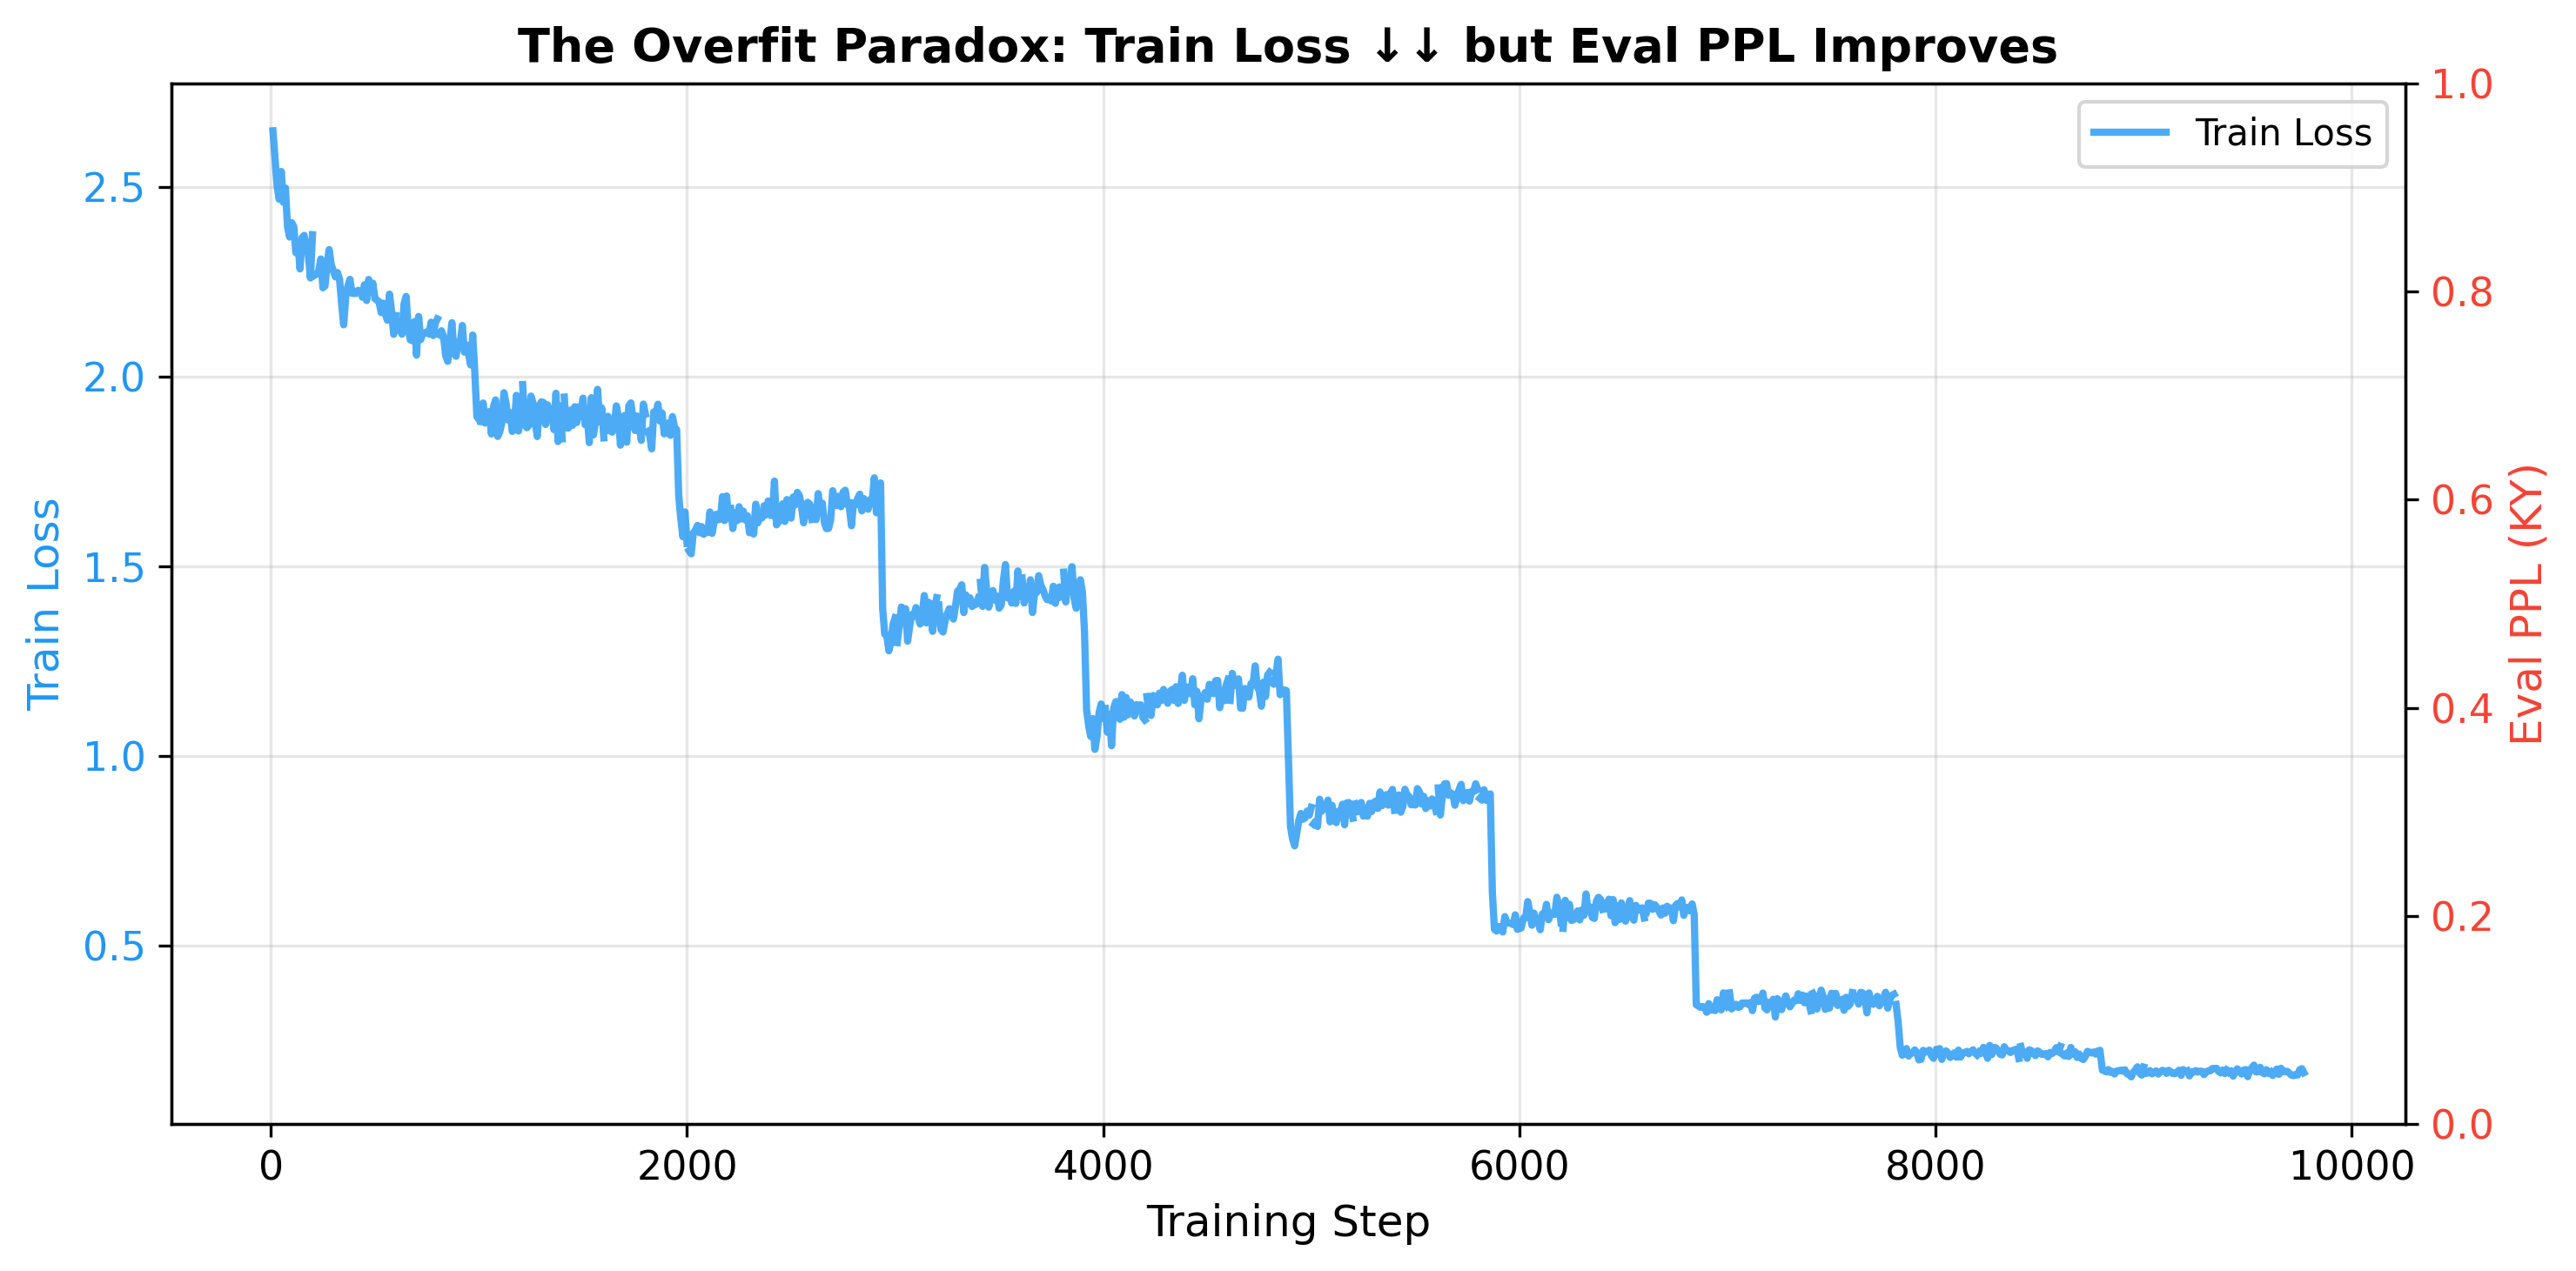
\includegraphics[width=0.85\textwidth]{../figures/fig7_overfit_paradox.png}
    \caption{The overfit paradox: 10 epochs of Kyrgyz training (E4) yields better target-language PPL (4.18 vs.\ 4.78) despite increasing cross-lingual degradation. Train loss continues to decrease while cross-lingual PPL rises monotonically.}
    \label{fig:overfit}
\end{figure*}

However, this improvement comes at a steep cost in cross-lingual knowledge. Kazakh PPL nearly doubles (87.65 vs.\ 47.58), Uzbek PPL increases by 68\% (95.76 vs.\ 56.85), and TUMLU accuracy on Kazakh drops from 30.2\% to 27.8\%. The spectral profile remains healthy throughout all 10 epochs (SE $< 0.5$), further confirming that SE is not a reliable indicator of training pathology.

This pattern suggests a regime of ``useful overfitting'' for the target language: the model memorizes patterns specific to Kyrgyz text more deeply, yielding better held-out perplexity on in-distribution data, but at the expense of broader multilingual competence. For practitioners focused on a single target language, extended training may be acceptable; for those seeking to maintain multilingual capability, it represents a significant regression. The directional analysis of \Cref{sec:directional} suggests an additional interpretation: extra epochs do not pin the adapter in a better direction, they extend movement along the seeded random one---an interpretation consistent with the lack of cross-seed directional reproducibility in direct-from-base training.

% ============================================================================
% 5. ANALYSIS AND DISCUSSION
% ============================================================================
\section{Analysis and Discussion}

\subsection{Why Spectral Energy Fails as a Diagnostic}

The failure of the SE threshold can be understood through the mathematics of LoRA initialization. Standard LoRA initializes $A$ with Kaiming uniform and $B$ with zeros. After the first gradient update, $B$ acquires small random-scale singular values with roughly uniform magnitudes, yielding $\text{SE} \approx 1/r$. As training progresses, all singular values grow, but the growth is typically distributed across multiple directions, causing $\text{SE}$ to remain stable or even \emph{decrease}.

For higher-rank configurations ($r{=}64$), the SE denominator includes more singular values, mechanically driving SE to lower values ($1/64 \approx 0.016$ at initialization versus $1/16 = 0.0625$ for $r{=}16$). Our empirical step-100 mean SE values track this prediction: $0.18$--$0.22$ at $r{=}16$ (E3, C3) versus $0.06$--$0.08$ at $r{=}64$ (E5, E5b, E5c), a roughly $3$--$4\times$ gap that is independent of any downstream functional outcome. This reveals SE as a \emph{rank-biased metric}: since $\text{SE} \approx 1/r$ at initialization, higher-rank adapters \emph{appear} spectrally healthier by definition, creating a dangerous trap for practitioners who monitor SE across configurations with different ranks. A seemingly healthy low-SE value for $r{=}64$ may actually correspond to a more pathological state than a higher SE for $r{=}16$.

The fundamental limitation is that SE is a \emph{shape} metric, invariant to rescaling of the singular value spectrum. A weight matrix with singular values $[100, 50, 25]$ and one with $[0.001, 0.0005, 0.00025]$ have identical SE, despite representing vastly different magnitudes of weight perturbation. In the low-resource setting, where models must substantially restructure their representations to accommodate poorly-covered languages, the \emph{scale} of these perturbations matters critically.

\Cref{fig:singular_values} visualizes the singular value distributions for representative experiments, illustrating how the $r{=}64$ configuration develops a well-distributed but extremely large-magnitude spectrum that SE fails to flag.

\begin{figure*}[t]
    \centering
    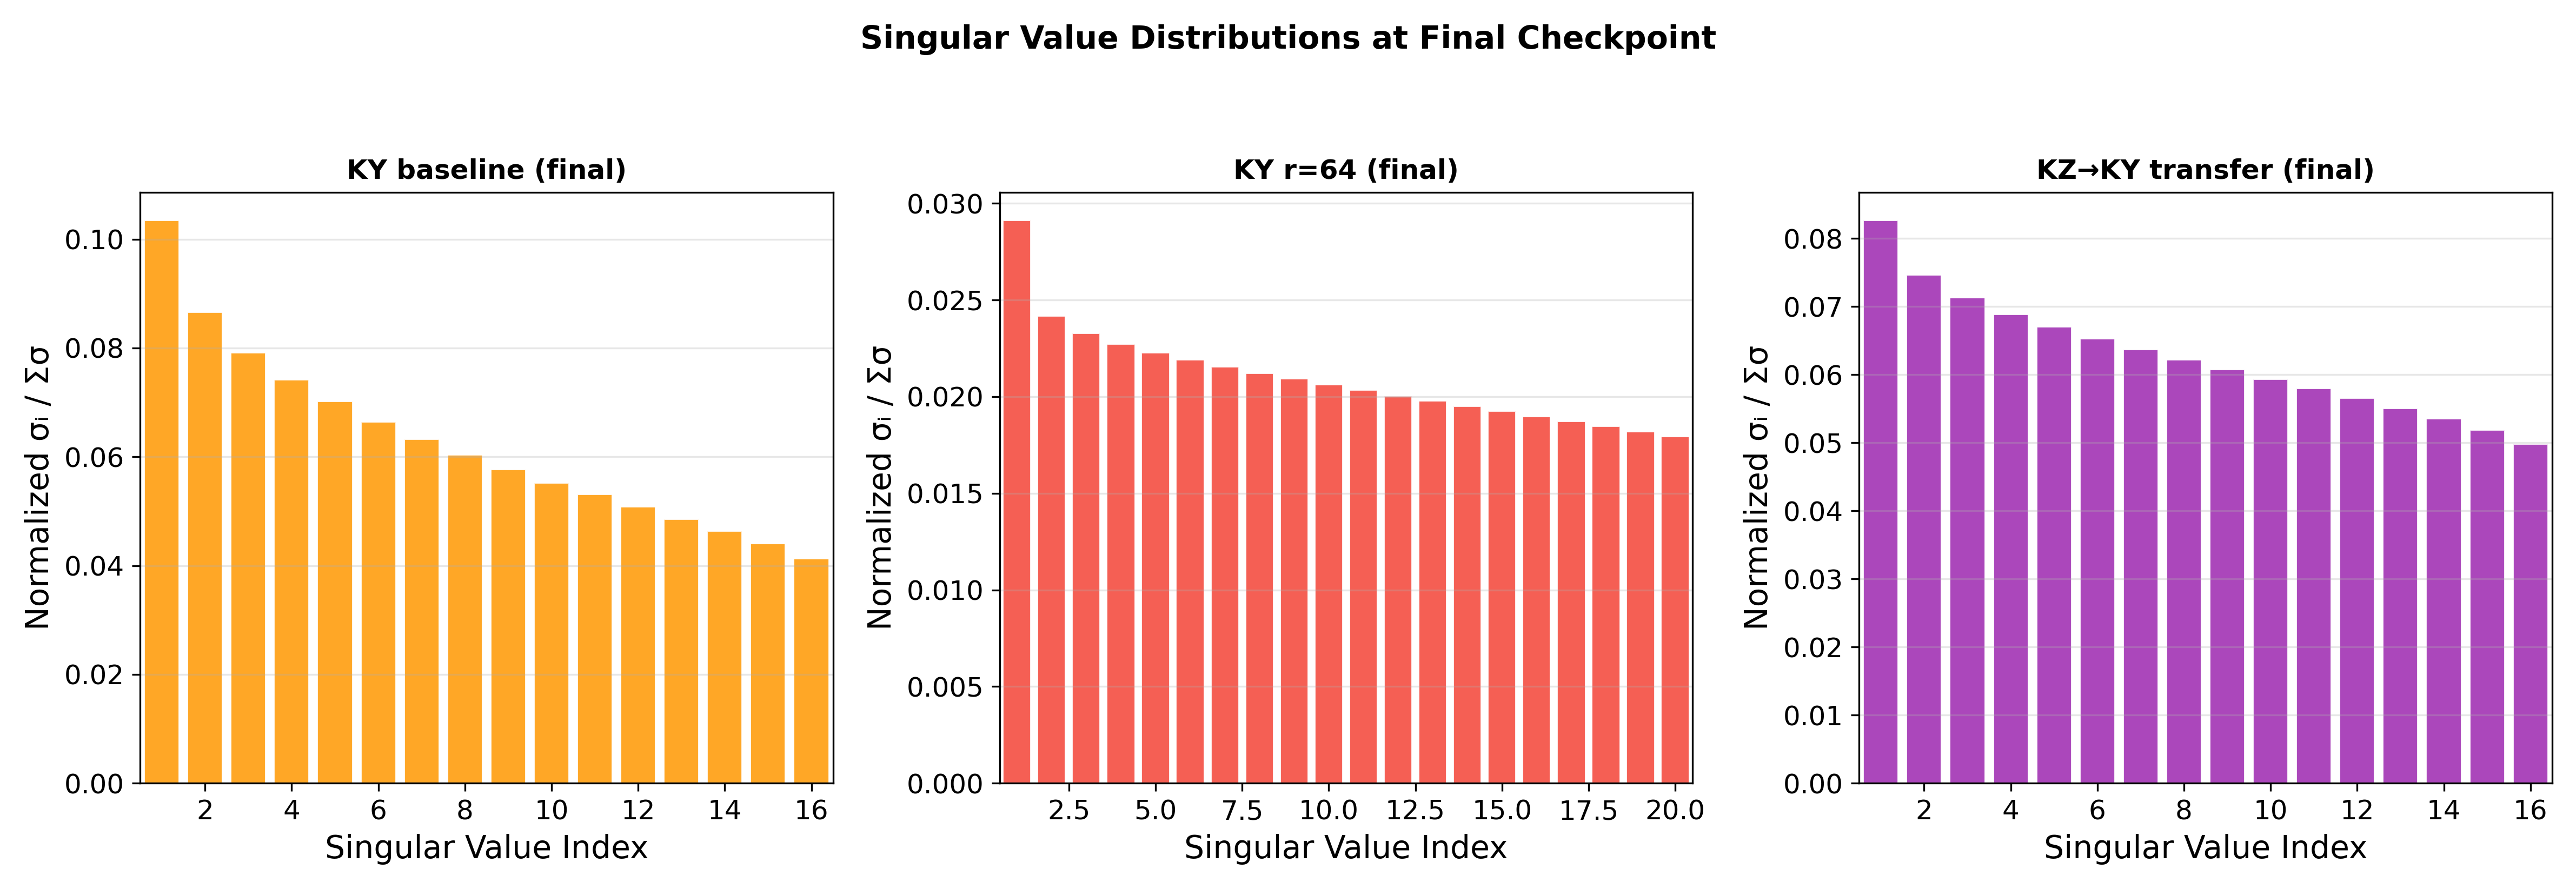
\includegraphics[width=\textwidth]{../figures/fig8_singular_values.png}
    \caption{Singular value distributions at the final checkpoint. The $r{=}64$ configuration (right) shows a well-distributed spectrum (low SE) with dramatically larger absolute magnitudes compared to the $r{=}16$ baseline (left), explaining why SE fails to detect pathological training.}
    \label{fig:singular_values}
\end{figure*}

\subsection{Underdetermination: No Final-Adapter Invariant Distinguishes Collapse from Healthy}
\label{sec:underdetermination}

The pairwise-cosine data of \Cref{sec:directional} support a stronger negative claim than ``SE is the wrong shape metric.'' We argue that \emph{no} continuous scalar function of the final adapter alone can reliably distinguish E5 (collapse) from E5c (healthy) at $r{=}64$ in this regime.

\textbf{The argument.} Let $D : (A, B) \mapsto \mathbb{R}$ be any candidate diagnostic computed from the final LoRA factors, and assume $D$ is Lipschitz with constant $L$ under any reasonable weight-space metric (Frobenius, cosine, or any invariant derived from $A^{\top}A$, $B^{\top}B$, or $BA$). For $D$ to reliably classify configurations $c_1$ (collapse) and $c_2$ (healthy), the between-configuration gap $\Delta_{D} = |D(A^{c_1}, B^{c_1}) - D(A^{c_2}, B^{c_2})|$ must exceed the within-configuration spread $\sigma_{D}^{\text{seed}} = \mathrm{std}_{s}[D(A^{c, s}, B^{c, s})]$ by a margin sufficient to separate the two classes.

Our pairwise cosines provide a direct lower bound on $\sigma_{D}^{\text{seed}}$ for any Lipschitz $D$. Within a single configuration, two seeds produce adapters whose per-module direction is essentially orthogonal: $1 - \cos$(E5, E5)$ \;=\; 0.978$, $1 - \cos$(E5c, E5c)$ \;=\; 0.968$. Between configurations, the analogous distance is no larger: $1 - \cos$(E5, E5c)$ \;=\; 0.990$. The between-class separation and the within-class spread are commensurate. Any Lipschitz $D$ therefore satisfies $\sigma_{D}^{\text{seed}}/\Delta_{D} \gtrsim 1$, i.e., its signal-to-noise ratio is bounded below order unity, and cannot place a stable decision boundary between the two regimes.

\textbf{Scope of the claim.} This rules out every scalar diagnostic in the family of (a) spectral-shape metrics applied to $A$, $B$, or $BA$ (SE, effective rank, stable rank, SVD entropy), (b) Frobenius-style scale metrics ($\|A\|_F$, $\|B\|_F$, $\|BA\|_F$), and (c) direction-based comparisons against any fixed reference (subspace alignment with $W_0$, projection energy onto pretrained top-$k$). All are continuous in $(A, B)$ under the relevant invariants, and all therefore inherit the same noise floor from cross-seed direction variance. Empirically, our v1 (top-$r$ subspace alignment with $W_0$) and v2 (cos$(BA, W_0)$, top-256 alignment) probes did fail to discriminate E5/E5c, consistent with this prediction.

\textbf{What can therefore work.} The argument is not nihilistic: it isolates the place where discrimination has to come from. Anything that breaks the Lipschitz-in-$(A, B)$ assumption is admissible. \emph{Functional} probes---cross-lingual PPL, NER F1, log-likelihood typing---are computed against held-out data, not the adapter weights alone, and can resolve the regimes (\Cref{tab:main_results}). \emph{Trajectory} probes that integrate gradients over training, rather than reading off the final adapter, are also outside the argument. The structural conclusion is that the final-adapter weight space is underdetermined: any seed of a healthy run looks just as different from any other healthy run as the average healthy run looks from a collapsed run, and no fixed-point geometry can break this symmetry.

\textbf{Why transfer initialisation is the exception.} The seed-orthogonality observed in (D1) is a property of direct training from raw base; once a non-trivial init pins the adapter's starting direction (E6: warm-started from KZ; E6b: warm-started from EN), cross-seed variance collapses (E6 cross-seed $\cos = 0.785$, $294/294$ modules above $0.5$). The optimization no longer samples uniformly from the sphere of orthogonal solutions, because the trajectory begins inside a much narrower cone. This is the structural counterpart of our retention finding (\Cref{sec:transfer}): transfer initialisation is a regularizer of \emph{direction}, not only of \emph{magnitude}, and it is the unique observed intervention in our 22-pair sweep that does so.

\subsection{Mechanistic Context: How This Relates to Prior Work}
\label{sec:mechanistic}

The two findings we develop above---structural underdetermination of the final LoRA adapter, and directional pinning by transfer initialisation---sit at the intersection of three lines of prior work that we briefly connect.

\textbf{Loss-surface geometry and mode connectivity.} \citet{garipov2018loss} and \citet{frankle2020linear} showed that independently trained networks on the same task often occupy distinct minima connected only by non-trivial paths through the loss surface, and that linear mode connectivity emerges only after a stability point in training. Our cross-seed cosines for direct LoRA fine-tuning ($\sim 0.02$--$0.04$, $0/294$ modules above $0.5$ in every direct configuration) are the LoRA-update analogue of this observation: two seeds of an identical configuration end up in essentially orthogonal regions of $BA$ space, indicating that the adapter optimisation does not enter a single shared basin from base initialisation. The transfer-initialised regime (E6, cross-seed cosine $0.785$, $294/294$ above $0.5$) is, in this language, evidence of a \emph{linearly connected} fine-tuning regime: starting from a non-trivial pinning point produces a single shared cone of solutions whose endpoint is reproducible across seeds. We do not attempt to formally test linear-mode-connectivity in our LoRA setting; the empirical contrast between the two regimes is itself the observation.

\textbf{Intrinsic dimensionality.} \citet{aghajanyan2021intrinsic} showed that LLM fine-tuning operates in a very low intrinsic dimension---a small number of directions in parameter space suffice to recover most of the task gain. A natural reading of our directional non-canonicity is that the low intrinsic dimension is a property of the \emph{loss landscape}, not of any specific axis: there are many low-dimensional subspaces that produce equivalent target-language fit, and direct LoRA training selects among them stochastically through seed/initialisation. The bimodality of our 22-pair cosine sweep then tells us \emph{which} subspace is selected is what differs across seeds, not \emph{how large} it is. The shape (singular-value distribution) is rank-biased and similar across runs; the spatial orientation is not.

\textbf{Fine-tuning distorts pretrained features.} \citet{kumar2022finetuning} argued that full fine-tuning can distort pretrained features in ways that hurt out-of-distribution behaviour, and that linear-probe-then-fine-tune (LP-FT) mitigates this. Our cross-lingual forgetting under direct LoRA training is consistent with feature distortion in their sense: large $\|B\|_F$ growth on a Turkic adapter induces high cross-lingual perplexity on the other Turkic languages, despite SE remaining well below threshold. Our transfer-initialisation finding suggests an analogue of LP-FT for the low-resource cross-lingual setting: a warm-start adapter functions as an initialisation that has already paid most of the distortion cost on a related task, so the residual fine-tuning lives in a narrower cone and disturbs fewer pretrained directions. The contrast E6 vs.\ E6b (related-language vs.\ cross-family warm-start) further suggests that the regularising effect is graded in the distance between the source and target tasks: cross-family E6b reaches $\cos = 0.343$ across seeds and partial KZ-retention, the related-family E6 reaches $0.785$ and full retention.

\textbf{LoRA initialisation work.} PiSSA \cite{meng2024pissa} initialises LoRA factors from a truncated SVD of $W_0$, biasing the adapter toward already-important pretrained directions; LoRA+ \cite{hayou2024loraplus} adjusts learning rates of $A$ vs.\ $B$ to address the asymmetry of the LoRA factorisation. Both are direction-pinning interventions in the sense above: they constrain where the optimisation can start (PiSSA) or how it can move (LoRA+). Our directional analysis suggests an empirical question for that line of work: do PiSSA or LoRA+ produce cross-seed cosines comparable to our E6 ($\sim 0.78$), or do they sit in the partial regime of E6b? We do not run those experiments here, but the per-module pairwise-cosine protocol of \Cref{sec:directional} provides a direct test.

What this prior work does \emph{not} say---and what we add---is the empirical structural claim that within standard direct LoRA fine-tuning the directional non-canonicity is large enough to set the noise floor on any final-adapter-geometric diagnostic (\Cref{sec:underdetermination}). The connection between this noise floor and the cross-lingual catastrophic-forgetting phenomenology is, to our knowledge, novel.

\subsection{Frobenius Norm as a Scale-Aware Alternative}

The Frobenius norm, $\|W\|_F = \sqrt{\sum_i \sigma_i^2}$, naturally captures the scale of weight perturbations that SE discards. Its squared value equals the sum of squared singular values, providing a direct measure of the total energy in the weight update. The Frobenius norm growth ratio (final/initial) thus quantifies how much the adapter has perturbed the pretrained weights.

Rather than prescribing fixed thresholds, we report the observed growth ranges in our experiments and caution that any such numbers are derived \emph{post hoc} from the same data used to define them, requiring held-out validation before deployment as decision rules:
\begin{itemize}
    \item \textbf{Transfer initialization} (E6): $1.13\times$---negligible additional perturbation atop an already-adapted checkpoint.
    \item \textbf{$r{=}16$ baselines on Turkic} (E3): $8\times$, with significant cross-lingual forgetting.
    \item \textbf{$r{=}16$ on well-represented language} (E8, EN): $33\times$, with minimal cross-lingual forgetting.
    \item \textbf{$r{=}16$ on higher-resource Turkic} (E1, KZ): $38\times$, with moderate forgetting.
    \item \textbf{$r{=}64$, high LR} (E5): $15$--$38\times$ over longer training, with complete functional collapse.
    \item \textbf{Diverged training} (E7): unbounded exponential growth, reaching $19\times$ in just 800 steps before divergence.
\end{itemize}

These growth ratios refer to $\|B\|_F^{\text{final}}/\|B\|_F^{\text{init}}$ and are normalized across initialization schemes (standard LoRA, PiSSA \cite{meng2024pissa}, or transfer), making the relative measure more portable than absolute norms.

\textbf{Why we do not propose fixed numeric thresholds.} The $33\times$ versus $38\times$ contrast between EN and KZ baselines---same magnitude, opposite forgetting outcomes---is the central caution: a single threshold applied across language categories would misclassify at least one of these regimes. Rather than a pass/fail number, we suggest practitioners (i) track the \emph{trajectory} of $\|B\|_F$ growth across training rather than a single endpoint value, (ii) flag \emph{super-linear} growth patterns (particularly exponential profiles, as in E7) as early warnings of divergence independent of magnitude, and (iii) always pair norm monitoring with a cross-lingual perplexity probe, since norm growth alone cannot resolve the well-represented vs.\ underrepresented asymmetry we document. Converting these observations into validated thresholds requires replication on held-out configurations and additional language families, which we leave to future work.

\subsection{Role of Subword Fragmentation}

The 3.2$\times$ subword fragmentation ratio observed for all three Turkic languages has several compounding effects on LoRA adaptation:

\textbf{Sequence length inflation:} A Kyrgyz sentence of 50 words requires approximately $50 \times 3.69 = 185$ tokens, versus $50 \times 1.15 = 58$ tokens for the English equivalent. With a maximum sequence length of 256 tokens, each training example contains substantially less textual content, reducing the information density of each gradient update.

\textbf{Morphological fragmentation:} Agglutinative suffixes that carry grammatical meaning are split across multiple subwords, forcing the model to reconstruct morphological relationships across token boundaries. For instance, a single Kazakh word form may be split into 4--5 subwords, with the root, derivational suffixes, and inflectional endings each occupying separate tokens.

\textbf{Link to forgetting severity.} Our EN control experiment (E8) shows a striking dissociation between norm growth and forgetting: comparable Frobenius growth (EN: 33$\times$ vs.\ KZ: 38$\times$) but minimal vs.\ severe cross-lingual degradation. We initially hypothesised this reflected directionality of the weight updates---Turkic fine-tuning restructuring representations in regions poorly covered by pretraining, while EN reinforces already well-represented features. The geometric probes of \Cref{sec:directional} only partially bear this out: cross-language pairs at $r{=}16$ (E1/E2/E3 mutual) sit at $\cos \approx 0.001$--$0.002$, below same-language cross-seed pairs, so different-language updates do rotate to fresh axes. However, the same-language cross-seed cosines for direct training are also $\approx 0.02$--$0.04$, so directionality is not what separates the EN-without-forgetting regime from the KZ-with-forgetting one---it is the pre-training coverage at the \emph{target} of each update that matters, regardless of the direction. Subword fragmentation provides a plausible mechanism for why Turkic updates would be more disruptive (more tokens per word means more constituent representations to modify), but we cannot isolate this from other factors with present data.

\subsection{Practical Recommendations}

Based on our findings, we offer the following recommendations for practitioners fine-tuning LLMs on low-resource, morphologically complex languages:

\begin{enumerate}
    \item \textbf{Do not gate fine-tuning health on spectral-energy thresholds.} The same near-zero SE coexists with healthy and collapsed behaviour at $r{=}64$ in our setting (\Cref{sec:spectral}); SE is a rank-biased shape metric that does not track functional outcomes.
    \item \textbf{Monitor Frobenius norm growth trajectories} rather than single endpoint values, and flag super-linear or exponential patterns as early-warning signals of divergence. We deliberately do not prescribe fixed numeric cut-offs: the same growth ratio ($33$--$38\times$) can coexist with or without forgetting depending on language representedness (\Cref{sec:frobenius}).
    \item \textbf{Treat collapse detection as a functional test} (cross-lingual PPL, NER, TUMLU). The underdetermination argument of \Cref{sec:underdetermination} shows that no Lipschitz function of the final adapter alone can substitute for it; the within-class noise floor from cross-seed direction variance is commensurate with the between-class gap.
    \item \textbf{Avoid aggressive rank--LR combinations} for small corpora ($\sim$150~MB). The combination of $r{=}64$ with $\text{lr} \geq 5 \times 10^{-4}$ leads to functional collapse in our setting, even when standard spectral metrics appear healthy. Note that E5 confounds rank and learning rate; the E5b/E5c controls show that the proximate cause is LR, not rank (\Cref{sec:spectral-collapse-rank-lr}).
    \item \textbf{Use related-language transfer initialisation} when available. It is the only intervention in our sweep that yields cross-seed reproducible LoRA directions (\Cref{sec:directional}), and it also recovers source-language perplexity with minimal additional Frobenius growth ($+13\%$ vs.\ $8\times$ for direct training).
    \item \textbf{Apply cross-lingual perplexity monitoring} as a forgetting diagnostic. Target-language PPL alone is insufficient; catastrophic forgetting manifests primarily in non-target languages.
    \item \textbf{Consider early stopping by cross-lingual PPL}, not training loss. Extended training may improve target-language metrics while severely degrading multilingual capability (\Cref{sec:overfit}).
\end{enumerate}

% ============================================================================
% 6. LIMITATIONS
% ============================================================================
\section{Limitations}
\label{sec:limitations}

Our study has several important limitations, which we discuss here in decreasing order of severity for downstream interpretation.

\textbf{(L1) Limited-seed experiments.} Most configurations in Table~\ref{tab:experiments} are run once ($n{=}1$). We provide $n{=}2$ seed-replicated runs (seeds 42 and 123) for the eight configurations underlying our main quantitative claims: E1b (small-corpus KZ), E3 (KY baseline), E5 (catastrophic collapse), E5b (rank--LR control), E5c (epoch-matched rank control), E6 (KZ$\rightarrow$KY transfer), E6b (EN$\rightarrow$KY cross-family control), and E8 (EN control); the full comparison is in \Cref{app:seed_variance}. The two-seed data confirm six claims that are consistent across both seeds: (a) the $2\times$ cross-lingual Kazakh-PPL retention effect of related-language transfer ($50.0\pm 2.4$ direct vs.\ $23.5\pm 0.1$ E6 transfer); (b) cross-family transfer does \emph{not} reproduce this retention (E6b: $48.8 \pm 1.4$, within direct-training spread); (c) E5c outperforms E3 at matched conditions (KY PPL $3.89 \pm 0.03$ vs.\ $4.81 \pm 0.03$); (d) the rank--LR disentanglement (E5b outside E5's collapsed regime in both seeds); (e) the E1b data-vs-coverage decomposition (KZ PPL $4.16 \pm 0.01$); and (f) the EN-vs-Turkic Frobenius dissociation (E8 $33.3 \pm 0.1\times$ growth with KZ PPL $5.52 \pm 0.02$ across seeds, vs.\ KZ baseline's $38.5\times$ with severe forgetting). With $n{=}2$ we report differences as consistent-across-two-seeds rather than as population-variance estimates; the absence of evidence for a sampling-distribution claim is not evidence of robustness, and we caution readers accordingly. Replication of E1, E2, E4, and the BF16 control C3 at $n{\geq}3$ would further tighten these numbers; for the remaining configurations our claims are explicitly framed as directional rather than precise.

\textbf{(L2) Training-set contamination for NER (quantified).} Our Turkic training corpora include Wikipedia dumps, and the WikiANN evaluation set is itself derived from Wikipedia entity links \cite{pan2017cross}. To quantify this overlap, we computed the fraction of unique gold WikiANN-test entity strings that appear verbatim somewhere in each training corpus (case-insensitive substring match): \textbf{Kazakh 65.7\% (497/757), Kyrgyz 55.9\% (52/93), Uzbek 2.2\% (13/602)}. The Kazakh and Kyrgyz NER F1 numbers in \Cref{tab:main_results} therefore upper-bound the contribution of memorization at $\sim$60\%, and cross-configuration NER comparisons within those two languages are partially confounded by this shared-entity floor. The Uzbek overlap of $2\%$, by contrast, is below the resolution of memorization (this turns out to be a script-mismatch artifact---see L9---which makes Uzbek a clean cross-lingual probe). The transfer-induced UZ improvements in \Cref{tab:main_results} (e.g., E1's $0.578$ F1 on UZ) are thus most likely \emph{not} memorization. A non-Wikipedia NER benchmark such as KazNERD \cite{yeshpanov2022kaznerd} (gated; access pending) would tighten this further; the per-type breakdown is reported in \Cref{app:overlap}.

\textbf{(L3) Rank--LR--epoch confound (now closed by E5b, E5c, and C5).} Experiment E5 ($r{=}64$, $\text{lr}{=}5\times 10^{-4}$, 5 epochs, $\alpha{=}128$) originally varied four factors. E5b matches rank but lowers LR; E5c additionally matches epoch count; C5 additionally matches $\alpha$. Together they decompose the variation cleanly (\Cref{sec:spectral-collapse-rank-lr}). Catastrophic collapse $=$ aggressive base LR (refuted by E5b). Extra cross-lingual forgetting $=$ training duration (refuted by E5c). \emph{Apparent} rank-only target-language advantage $=$ implicit LR boost from $\alpha/r=2$ (refuted by C5: at $\alpha{=}32$, $r{=}64$ is indistinguishable from the $r{=}16$ baseline on KY/KZ/UZ PPL, NER F1, and TUMLU). Rank itself, at matched effective LR, does not deliver a functional benefit in our setting.

\textbf{(L4) Quantization confound (addressed by C3).} The original concern was that 4-bit NF4 quantization might suppress singular-value growth, making our sub-threshold SE observation an artefact of precision rather than language-specific dynamics. The C3 BF16 control (Kyrgyz, $r{=}16$, $\text{lr}{=}2\times 10^{-4}$, 3 epochs, identical to E3 except for full-precision base model) refutes this: BF16 SE behaviour is statistically indistinguishable from 4-bit E3 at every comparable point---final max SE $0.32$ vs.\ $0.33 \pm 0.01$, final mean SE $0.10$ in both, and in-training peak max SE $0.47$ vs.\ $0.45 \pm 0.02$ (\Cref{tab:bf16}). Frobenius growth, KY PPL, NER F1, log-likelihood span typing, and TUMLU accuracy are likewise within seed-level variance of E3 (\Cref{app:bf16}). Quantization is therefore not artificially suppressing SE---and is not the explanation for the SE-threshold falsification. The residual gap is that we ran C3 only at $n{=}1$ (cloud GPU cost); a second BF16 seed would tighten the comparison further.

\textbf{(L5) Corpus imbalance between Turkic languages (partially addressed by E1b).} We match corpora by raw byte size ($\sim$150~MB each), yet token counts differ substantially after tokenization (KZ: 14.1M, UZ: 5.4M, KY: 4.4M). To isolate tokenizer-coverage effects from raw-data-volume effects, we ran a small-corpus Kazakh control E1b on $\sim$1.5M training tokens (the corpus was sized via a word$\times$fragmentation-ratio estimate aiming for the KY 4.4M target; the actual chunked-token count came out lower). Result: target KZ PPL rises from $2.73$ (E1) to $4.17$ (E1b) with the smaller corpus, confirming that data volume materially contributes to the E1 advantage. Importantly, E1b's $4.17$ remains lower than the Kyrgyz baseline's $4.78$ even though E1b trained on $\sim 3\times$ \emph{fewer} tokens than KY---so Kazakh also enjoys a genuine tokenizer-/pretraining-coverage advantage that is not attributable to corpus size. Both factors contribute; neither alone explains the gap. A parallel control on Uzbek data, and a true 4.4M-token Kazakh control, would tighten this further; we defer them to future work.

\textbf{(L6) NER as a primary metric.} Our NER evaluation uses 3-shot prompting with $n{=}100$ samples per language and F1 derived from parse-success output. This is closer to a test of instruction-following than of entity knowledge. The $r{=}64$ ``NER F1 $= 0$'' result, in particular, is driven by 100\% parse failures; the model may retain some entity knowledge that this evaluation cannot access. Log-likelihood-based NER scoring (scoring candidate entity spans by model probability) would separate instruction loss from knowledge loss and is a priority follow-up.

\textbf{(L7) Scope of generalization.} All experiments use a single base model (Gemma-2-9B); the bimodal directional structure of \Cref{sec:directional}---direct training at cross-seed $\cos \approx 0.03$, transfer-init at $\cos \approx 0.78$---is established only on this architecture and should be replicated on Llama-3 or Mistral before being claimed as architecture-independent. We examine only three of the approximately 35 Turkic languages, excluding Turkish (the highest-resource Turkic language). Corpus size is fixed at $\sim$150~MB per language, precluding scaling analyses. SVD monitoring focuses on $\texttt{lora\_B}$; the pairwise-cosine analysis is computed on the full $\Delta W{=}BA$ and so does not depend on this choice.

\textbf{(L8) Post-hoc Frobenius observations.} The growth ranges in Section~\ref{sec:frobenius} are derived from the same experiments on which their interpretation is built; they are observations requiring held-out validation, not established thresholds, and we deliberately reframe them as such in Section~\ref{sec:frobenius}.

\textbf{(L9) Uzbek script coverage.} Our Uzbek training corpus is restricted to Cyrillic-script sources, while WikiANN-uz uses primarily Latin script: this is the most likely explanation for the $2\%$ entity-string overlap reported in L2 (vs.\ $\sim 60\%$ for KZ/KY where script alignment is uniform Cyrillic). Since Uzbekistan officially uses Latin script and most contemporary formal text is Latin-based, our Uzbek perplexity and target-language NER results should not be generalized to Latin-script data without a separate evaluation. The script-mismatch nonetheless gives us an unintended benefit: Uzbek serves as a cleaner cross-lingual probe than KZ or KY because memorization-driven inflation is negligible, so the strong transfer-induced UZ improvements (e.g., E1's $0.578$ F1) are difficult to attribute to data leakage.

% ============================================================================
% 7. CONCLUSION
% ============================================================================
\section{Conclusion}

We have presented a systematic study of the spectral and directional dynamics of LoRA adapters during fine-tuning on three low-resource Turkic languages. Our experiments yield four principal findings.

First, the spectral-energy threshold of \citet{biderman2024lora} is \textbf{not predictive} in our regime. The E5/E5b/E5c/C5 four-way decomposition shows that at matched rank ($r{=}64$), four runs converging to settled spectral trajectories below the threshold (final max SE $0.06$--$0.24$, final mean SE $\sim 0.03$--$0.05$) span the full functional range from catastrophic collapse (E5: F1$=0$, TUMLU $23\%$) to behaviour matching the $r{=}16$ baseline (C5: KY PPL $4.46$, KZ PPL $49$). SE cannot detect the difference. The C3 BF16 control rules out 4-bit quantization as the cause: BF16 SE behaviour is statistically indistinguishable from 4-bit E3 (\Cref{tab:bf16}), so the sub-threshold values are not an artefact of precision. The C5 control (matched effective LR at $\alpha{=}32$) additionally reveals that the apparent rank-only benefit of E5c over E3 ($3.86$ vs.\ $4.78$ KY PPL) was an artefact of the standard $\alpha/r=2$ practice: at $\alpha{=}32$, $r{=}64$ is functionally indistinguishable from $r{=}16$. Higher rank in standard practice acts as a proxy for higher effective LR, not as an independent capacity dimension.

Second, \textbf{Frobenius norm growth} is a useful scale-aware monitoring signal but \emph{not} a universal diagnostic. Within underrepresented languages it reliably separates regimes ($1.13\times$ for transfer vs.\ $15$--$38\times$ for high-LR $r{=}64$). Across language categories it fails: our English control absorbs $33\times$ norm growth with minimal forgetting, comparable to Kazakh's $38\times$ \emph{with} forgetting. We therefore recommend pairing $\|\mathbf{B}\|_F$ trajectory monitoring with cross-lingual PPL probes rather than relying on fixed thresholds.

Third, the previous two findings are special cases of a broader \textbf{structural underdetermination} of the LoRA solution. A 22-pair sweep of per-module cosines between $\Delta W{=}BA$ matrices shows that direct LoRA fine-tuning from base lands in a near-orthogonal direction for every seed: same-configuration cross-seed cosines cluster at $0.01$--$0.04$ ($0/294$ modules above $0.5$ in all six tested setups), and the collapse-vs-healthy gap (E5 vs.\ E5c, cosine $0.010$) is no larger than two seeds of either condition. From this we derive a formal impossibility (\Cref{sec:underdetermination}): no Lipschitz scalar function of the final adapter alone---SE, Frobenius, effective rank, alignment with $W_0$---can resolve collapse from healthy training when its within-class noise floor (set by cross-seed direction variance) is commensurate with the between-class gap. Diagnosis of collapse must come from functional probes (cross-lingual PPL, NER F1) or trajectory probes (gradient cumulants), not from any geometry of the final weight.

Fourth, transfer initialisation is the \emph{only} intervention in our sweep that breaks this directional non-canonicity, and this re-frames our earlier retention finding. Kazakh$\rightarrow$Kyrgyz warm-start halves cross-lingual Kazakh PPL ($23.5 \pm 0.1$ vs.\ $50.0 \pm 2.4$ under direct training) while requiring only $+13\%$ Frobenius growth; the seed-replicated cross-family control (E6b: EN$\rightarrow$KY) does not reproduce this retention. Geometrically, E6 reaches cross-seed cosine $0.785$ with $294/294$ modules above $0.5$, while direct training stays at $0.04$---meaning warm-started training is reproducible across seeds in a way direct training is not, and this directional reproducibility is the structural signature that distinguishes the retention regime from the displacement regime.

These findings have immediate practical implications. The first three say that final-state spectral and Frobenius monitoring cannot replace cross-lingual perplexity probes for collapse detection in low-resource quantized LoRA; the fourth says that transfer initialisation should be considered not only when retention of a source language is desired but whenever reproducibility of LoRA fine-tuning across seeds is a practical concern. Future work should validate the bimodal directional structure across base models (Llama-3, Mistral), test whether alternative initialisations such as PiSSA \cite{meng2024pissa} approximate the transfer-init regime without an explicit source language, and develop trajectory-based diagnostics that fall outside the underdetermination argument.

% ============================================================================
% ETHICS STATEMENT
% ============================================================================
\section*{Ethics Statement}

This work involves fine-tuning language models on text corpora from three Turkic languages and English. While we aim to improve NLP capabilities for underserved language communities, we acknowledge that language models can amplify biases present in training data. Our training corpora, drawn from Wikipedia, literary texts, and web sources, may contain cultural biases or factual inaccuracies.

\textbf{Data availability:} The Kazakh and Uzbek corpora are compiled from publicly available sources (Wikipedia, open book collections). The Kyrgyz corpus is curated from licensed literary and encyclopedic sources and cannot be redistributed due to copyright restrictions. In the spirit of open science, we release all experimental code, SVD monitoring logs, and evaluation results via an anonymous repository.\footnote{\url{https://anonymous.4open.science/r/Spectral-Collapse-Turkic-Conference-14D8}}. Trained LoRA adapters will be publicly released upon acceptance to preserve author anonymity during review.

% ============================================================================
% ACKNOWLEDGMENTS
% ============================================================================
\section*{Acknowledgments}

We thank the creators of the Kazakh, Kyrgyz, and Uzbek corpora used in this study, as well as the developers of the TUMLU benchmark for providing standardized Turkic language evaluation resources. All experiments were conducted on personal hardware without external funding.

% ============================================================================
% REPRODUCIBILITY
% ============================================================================
\section*{Reproducibility Statement}

All experimental code (training with SVD monitoring, evaluation, and plotting scripts), SVD monitoring logs, and evaluation reports are publicly available at \url{https://anonymous.4open.science/r/Spectral-Collapse-Turkic-Conference-14D8}. Fine-tuned LoRA adapters for all eight experiments will be released on a public model hub upon acceptance to preserve author anonymity during review. The Kazakh, Uzbek, and English training corpora are derived from publicly available sources and can be reconstructed using the provided data preparation scripts. The Kyrgyz corpus cannot be redistributed due to licensing restrictions on its source materials; consequently, the KY training stage is not fully reproducible. However, the released KY adapters and SVD logs enable full reproduction of all evaluation and analysis stages.

% ============================================================================
% REFERENCES
% ============================================================================
\bibliography{references}

\appendix

% ============================================================================
% APPENDIX
% ============================================================================
\section{Detailed Training Configurations}
\label{app:configs}

All experiments were conducted on a single NVIDIA GeForce RTX 5080 (16~GB) using PyTorch 2.10, Transformers 5.2, and PEFT 0.18. \Cref{tab:training_details} provides the full training statistics.

\begin{table*}[t]
\centering
\small
\begin{tabular}{llccccc}
\toprule
\textbf{ID} & \textbf{Experiment} & \textbf{Train Loss} & \textbf{Eval Loss} & \textbf{Eval PPL} & \textbf{Tokens} & \textbf{Time (min)} \\
\midrule
E1 & KZ Baseline (14.1M) & 0.275 & 1.259 & 3.52 & 14.1M & 477 \\
E1b & KZ Small-corpus (1.5M) & 1.186 & 1.461 & 4.31 & 1.5M & 122 \\
E2 & UZ Baseline & 1.193 & 1.822 & 6.18 & 5.4M & 341 \\
E3 & KY Baseline & 0.815 & 1.920 & 6.82 & 4.4M & 183 \\
E4 & KY Overfit & 1.050 & 1.963 & 7.12 & 4.4M & 1193 \\
E5 & KY $r{=}64$ high-LR & 0.274 & 2.164 & 8.71 & 4.4M & 157 \\
E5b & KY $r{=}64$ std-LR (5ep) & 1.278 & 1.964 & 7.13 & 4.4M & 605 \\
E5c & KY $r{=}64$ epoch-matched & 1.652 & 1.898 & 6.67 & 4.4M & 360 \\
E6 & KZ$\rightarrow$KY & 1.809 & 1.932 & 6.90 & 4.4M & 355 \\
E8 & EN Control & 1.821 & 2.017 & 7.51 & 12.7M & 1351 \\
\bottomrule
\end{tabular}
\caption{Full training statistics for all experiments. Eval loss and PPL are computed on the validation split during training (distinct from the post-hoc evaluation in \Cref{tab:main_results}). The higher train loss for E6 (KZ$\rightarrow$KY) reflects the adapter starting from KZ-optimized weights that initially perform poorly on KY data.}
\label{tab:training_details}
\end{table*}

\section{Effective Rank Dynamics}
\label{app:effrank}

\Cref{fig:effrank} shows the effective rank dynamics across experiments. The $r{=}64$ configuration shows increasing effective rank (from $\sim$6 to $\sim$26), indicating growing parameter utilization. The diverged experiment (E7) is the only configuration where effective rank \emph{decreases} (from 43.3 to 37.1), consistent with true spectral collapse.

\textbf{E7 divergence analysis.} The diverged experiment ($r{=}64$, $\text{lr}{=}10^{-3}$) provides the most extreme datapoint. Training terminated at step 800 due to loss divergence. Even at this point, maximum SE was only 0.18---still far below the 0.7 threshold---while mean Frobenius norm had already reached 6.75 (19$\times$ growth in just 800 steps, compared to 15.6$\times$ over 4,885 steps for E5). The effective rank decrease (43.3 $\rightarrow$ 37.1) in the final 200 steps is the only instance of true rank contraction in our experiments, suggesting that SE-based collapse detection may only trigger \emph{after} the model has already diverged---too late for practical intervention. The Frobenius norm, by contrast, shows clear exponential growth from step 100 onward, providing a much earlier warning signal.

\begin{figure*}[t]
    \centering
    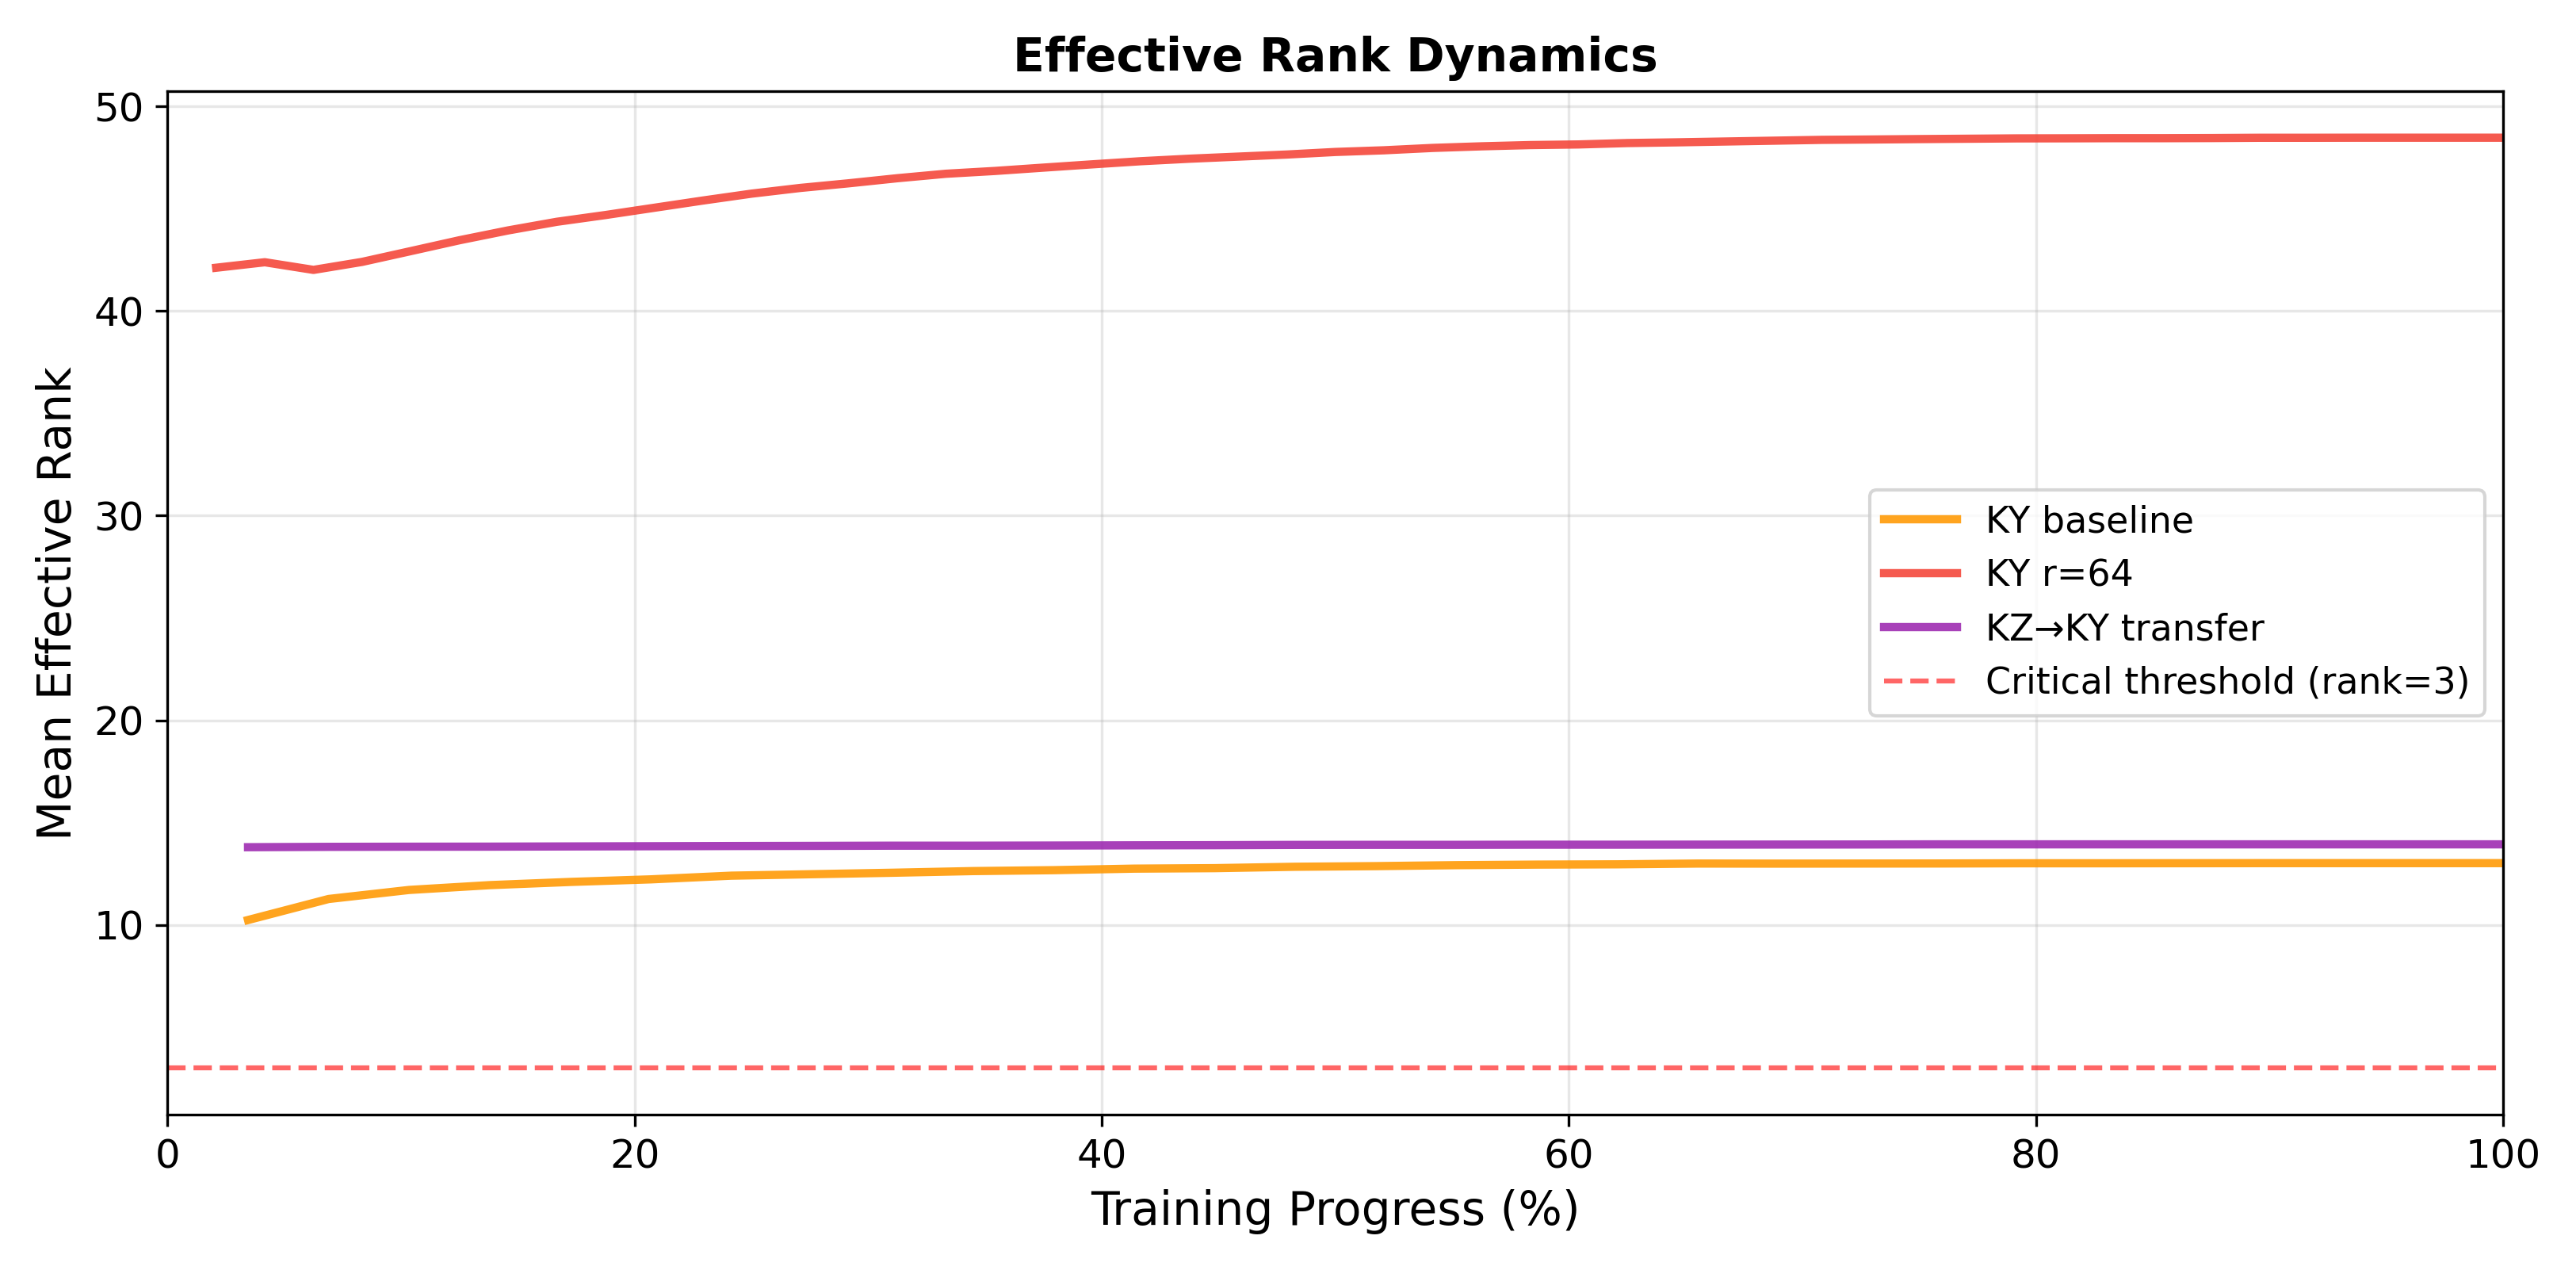
\includegraphics[width=\textwidth]{../figures/fig5_effective_rank.png}
    \caption{Effective rank dynamics during training. The $r{=}64$ configuration shows increasing effective rank despite functional degradation, further evidence that standard spectral metrics can be misleading.}
    \label{fig:effrank}
\end{figure*}

\section{Log-Likelihood NER: Type Classification under Gold Spans}
\label{app:ner_loglik}

To separate loss of entity knowledge from loss of instruction-following/output-formatting, we add a second NER evaluation that does not require the model to generate structured output. Given the gold-span boundaries from WikiANN, we present each span in context and score three candidate completions (``person'', ``organization'', ``location'') by log-likelihood under the adapter; the predicted type is the argmax. Because this evaluation never relies on the model's output format, it is immune to the 100\% parse-failure mode that drives E5's NER F1~$= 0$ under generation-based scoring.

\Cref{tab:ner_loglik} reports per-language type accuracy and macro-F1 on the same 100-example test sets used for \Cref{tab:main_results}.

\begin{table}[t]
\centering
\small
\begin{tabular}{lccc}
\toprule
\textbf{Experiment} & \textbf{KY} & \textbf{KZ} & \textbf{UZ} \\
\midrule
E1 KZ Baseline (14.1M tok)   & 57.7\% & 72.3\% & 70.9\% \\
E1b KZ Small-corpus (1.5M)   & 46.0\% & 70.5\% & 69.9\% \\
E2 UZ Baseline               & 54.9\% & 71.4\% & 65.0\% \\
E3 KY Baseline               & 50.4\% & 69.6\% & 63.1\% \\
E4 KY Overfit (10ep)         & 56.8\% & 71.4\% & 60.2\% \\
E5 KY $r{=}64$ (lr $5{\times}10^{-4}$)  & \textbf{59.5\%} & 50.0\% & 55.3\% \\
E5b KY $r{=}64$ 5ep (lr $2{\times}10^{-4}$) & 53.1\% & 70.5\% & 69.9\% \\
E5c KY $r{=}64$ 3ep (lr $2{\times}10^{-4}$) & 54.9\% & 67.9\% & 63.1\% \\
E6 KZ$\rightarrow$KY (related)   & \textbf{59.5\%} & \textbf{73.2\%} & 66.0\% \\
E6b EN$\rightarrow$KY (cross-family) & 54.0\% & 70.5\% & 70.9\% \\
E8 EN Control                & 56.8\% & \textbf{73.2\%} & 68.0\% \\
\bottomrule
\end{tabular}
\caption{Log-likelihood span-type accuracy across experiments (gold-span boundaries, argmax over \{PER, ORG, LOC\}). Random-baseline accuracy is 33.3\%. The parse-failure-immune evaluation reveals that \textbf{E5 retains and even marginally exceeds target-language (KY) entity knowledge} (59.5\%, tied for best with E6) despite scoring F1~$= 0$ under generation-based NER---confirming that the high-LR $r{=}64$ collapse destroys instruction-following, not entity knowledge itself. Cross-lingual degradation, however, does appear in E5 on non-target languages (KZ 50.0\% vs.\ 70--73\% for others), consistent with the cross-lingual PPL increase. Under this cleaner metric, the KZ$\rightarrow$KY transfer advantage over the KY baseline is modest (59.5\% vs.\ 50.4\% on KY; $+9.1$ absolute percentage points) rather than the $+61\%$ relative improvement suggested by generation F1, reinforcing our framing of cross-lingual transfer as a \emph{directional} rather than precise effect. Notably, the cross-family transfer E6b (EN$\rightarrow$KY) sits intermediate at $54.0\%$, consistent with cross-family initialization providing partial---but smaller---entity-knowledge benefit than related-language transfer.}
\label{tab:ner_loglik}
\end{table}

\section{WikiANN--Training Entity Overlap}
\label{app:overlap}

We quantify the entity-level overlap between each language's training corpus and the WikiANN test split it is evaluated on. For every gold span in the WikiANN test set we test whether the entity string appears verbatim (case-insensitive) anywhere in the corresponding training corpus. The unique-overlap rate is an upper bound on the fraction of NER F1 that could be explained by memorization of seen entity surface forms.

\begin{table}[t]
\centering
\small
\begin{tabular}{lccc}
\toprule
\textbf{Language} & \textbf{Total spans} & \textbf{Unique} & \textbf{Unique overlap} \\
\midrule
Kazakh (KZ)  & 1{,}115 & 757 & \textbf{65.7\%} (497/757) \\
Kyrgyz (KY)  & 111     & 93  & \textbf{55.9\%} (52/93) \\
Uzbek (UZ)   & 1{,}011 & 602 & \textbf{2.2\%}  (13/602) \\
\bottomrule
\end{tabular}
\caption{Verbatim case-insensitive overlap between WikiANN test entities and our training corpora. KZ and KY show high overlap (memorization upper bound $\sim 60\%$); UZ shows almost none, which we attribute to script mismatch between our Cyrillic UZ corpus and Latin-script WikiANN-uz (L9). The UZ low overlap incidentally turns Uzbek into a cleaner cross-lingual transfer probe: improvements in UZ NER are unlikely to be memorization artefacts.}
\label{tab:overlap}
\end{table}

\begin{table}[t]
\centering
\small
\begin{tabular}{lccc}
\toprule
\textbf{Language} & \textbf{PER} & \textbf{ORG} & \textbf{LOC} \\
\midrule
Kazakh & 71\% (221/313) & 62\% (170/276) & 63\% (106/168) \\
Kyrgyz & 33\% (11/33)   & 57\% (17/30)   & 80\% (24/30)   \\
Uzbek  & 3\% (2/67)     & 4\% (8/202)    & 1\% (3/333)    \\
\bottomrule
\end{tabular}
\caption{Per-type unique overlap. The KY pattern (LOC $\gg$ PER) is consistent with location names being a comparatively closed-class compared to person names. UZ remains uniformly low across types, confirming the script-mismatch explanation.}
\label{tab:overlap_per_type}
\end{table}

\section{BF16 vs.\ 4-bit Control (C3)}
\label{app:bf16}

\Cref{tab:bf16} reports a side-by-side comparison of the 4-bit E3 baseline (averaged across our two seeds where available) and the full-precision BF16 control (C3, single seed, run on a cloud A100~40GB instance). All hyperparameters except quantization are identical.

\begin{table}[t]
\centering
\small
\begin{tabular}{lcc}
\toprule
\textbf{Metric} & \textbf{E3 (4-bit, 2 seeds)} & \textbf{C3 (BF16, $n{=}1$)} \\
\midrule
KY PPL              & $4.81 \pm 0.02$    & $4.99$ \\
KZ PPL (cross-ling) & $50.0 \pm 2.4$     & $43.97$ \\
UZ PPL (cross-ling) & $55.5 \pm 1.4$     & $59.02$ \\
NER F1 KY (gen)     & $0.170 \pm 0.013$  & $0.164$ \\
NER TypeAcc KY      & $55.0 \pm 4.6$     & $58.6$ \\
TUMLU KY            & $36.1 \pm 1.4$     & $36.1$ \\
$\|B\|_F$ growth    & $8.36\times$       & $8.60\times$ \\
Final SE max        & $0.33 \pm 0.01$    & $0.32$ \\
Final SE mean       & $0.10$             & $0.10$ \\
Peak SE max (training) & $0.45 \pm 0.02$ & $0.47$ \\
\bottomrule
\end{tabular}
\caption{4-bit NF4 vs.\ BF16 control on the same KY baseline configuration (rank 16, lr $2{\times}10^{-4}$, 3 epochs). E3 (4-bit) values are reported as $\text{mean} \pm \text{half-range}$ across two seeds (seeds 42 and 123); we use half-range rather than standard deviation because the unbiased SD estimator at $n{=}2$ is unreliable, and half-range gives a more honest visual sense of seed-to-seed spread. All downstream metrics fall within or near this two-seed spread for the 4-bit run. Frobenius norm growth is essentially identical. Spectral energy in BF16 is statistically indistinguishable from 4-bit at every comparable point (final max, final mean, in-training peak), which rules out the original concern: 4-bit quantization is not artificially suppressing SE. The SE-threshold falsification therefore carries over to full precision. We did not run a second seed for C3 due to compute cost (the BF16 run was completed on rented cloud GPU); $n{=}1$ is acknowledged in L1.}
\label{tab:bf16}
\end{table}

\section{Seed-Variance Replication}
\label{app:seed_variance}

To provide at least partial seed-variance estimates for our most consequential configurations, we rerun two experiments under a second seed ($123$, while the originals used seed $42$). Training hyperparameters and data are identical across seeds; only the random seed for initialization, data shuffling, and train/val split differs.

\begin{table*}[t]
\centering
\scriptsize
\setlength{\tabcolsep}{1.8pt}
\begin{tabular}{lrrrrrrrrrrrrrrrr}
\toprule
 & \multicolumn{2}{c}{\textbf{E1b}} & \multicolumn{2}{c}{\textbf{E3}} & \multicolumn{2}{c}{\textbf{E5}} & \multicolumn{2}{c}{\textbf{E5b}} & \multicolumn{2}{c}{\textbf{E5c}} & \multicolumn{2}{c}{\textbf{E6}} & \multicolumn{2}{c}{\textbf{E6b}} & \multicolumn{2}{c}{\textbf{E8 (EN)}} \\
\cmidrule(lr){2-3}\cmidrule(lr){4-5}\cmidrule(lr){6-7}\cmidrule(lr){8-9}\cmidrule(lr){10-11}\cmidrule(lr){12-13}\cmidrule(lr){14-15}\cmidrule(lr){16-17}
\textbf{Metric} & s=42 & s=123 & s=42 & s=123 & s=42 & s=123 & s=42 & s=123 & s=42 & s=123 & s=42 & s=123 & s=42 & s=123 & s=42 & s=123 \\
\midrule
KY PPL $\downarrow$         & 25.55 & 28.81 & 4.78 & 4.83 & 5.90 & 6.01 & 4.55 & 4.62 & 3.86 & 3.92 & 4.73 & 4.78 & 4.78 & 4.83 & 14.96 & 14.82 \\
KZ PPL $\downarrow$         & \textbf{4.17} & \textbf{4.15} & 47.58 & 52.47 & 659.25 & 606.81 & 128.04 & 107.23 & 93.52 & 98.62 & \textbf{23.49} & \textbf{23.61} & 47.46 & 50.21 & 5.54 & 5.50 \\
UZ PPL $\downarrow$         & 23.17 & 21.93 & 56.85 & 54.05 & 742.73 & 763.79 & 162.68 & 139.89 & 111.25 & 96.61 & 124.19 & 114.54 & 63.42 & 57.51 & 16.55 & 16.28 \\
NER F1 KY (gen) $\uparrow$  & 0.150 & 0.139 & 0.157 & 0.182 & 0.000 & 0.000 & 0.146 & 0.116 & 0.115 & 0.169 & 0.253 & 0.179 & 0.133 & 0.110 & 0.209 & 0.227 \\
TypeAcc KY $\uparrow$       & 46.0 & 53.1 & 50.4 & 59.5 & 59.5 & 53.1 & 53.1 & 64.9 & 54.9 & 64.9 & 59.5 & 64.9 & 54.0 & 57.7 & 56.8 & 54.9 \\
TypeAcc KZ $\uparrow$       & 70.5 & 70.5 & 69.6 & 70.5 & 50.0 & 40.2 & 70.5 & 71.4 & 67.9 & 69.6 & 73.2 & 75.0 & 70.5 & 69.6 & 73.2 & 72.3 \\
TUMLU KY $\uparrow$         & 37.3 & 38.6 & 34.7 & 37.4 & 23.2 & 23.9 & 33.2 & 33.2 & 38.5 & 38.0 & 33.7 & 34.9 & 36.1 & 35.9 & 37.7 & 36.2 \\
$\|B\|_F$ growth            & 2.86$\times$ & 2.88$\times$ & 8.36$\times$ & 8.30$\times$ & 15.65$\times$ & 15.50$\times$ & 18.19$\times$ & 18.07$\times$ & 8.72$\times$ & 8.66$\times$ & 1.13$\times$ & 1.13$\times$ & 3.10$\times$ & 3.09$\times$ & 33.39$\times$ & 33.17$\times$ \\
\bottomrule
\end{tabular}
\caption{Two-seed replication for the eight configurations underlying our main claims: small-corpus KZ baseline (E1b, 1.5M tokens), KY baseline (E3), catastrophic collapse (E5), rank--LR control (E5b), epoch-matched control (E5c), related-language transfer (E6: KZ$\rightarrow$KY), cross-family transfer (E6b: EN$\rightarrow$KY), and EN control (E8). All TypeAcc values are percentages. Aggregate values reported elsewhere as ``$x \pm y$'' use the seed mean and half-range ($y = (\max-\min)/2$), not standard deviation, because the unbiased SD estimator at $n{=}2$ is unreliable; readers should interpret these as consistent-across-two-seeds spreads rather than population-variance estimates. \textbf{Six claims hold consistently across both seeds:} \textbf{(i)} \emph{related-language transfer halves cross-lingual KZ PPL} (E6: $23.5 \pm 0.1$ vs.\ E3 $50.0 \pm 2.4$, a separation $\sim 10\times$ larger than either condition's spread); \textbf{(ii)} \emph{cross-family warm-start does not reproduce this retention} (E6b: KZ PPL $48.8 \pm 1.4$, within seed spread of direct training, far above E6); \textbf{(iii)} \emph{r=64 outperforms r=16 baseline at matched conditions} (E5c KY PPL $3.89 \pm 0.03$ vs.\ E3 $4.81 \pm 0.03$); \textbf{(iv)} \emph{rank-LR disentanglement} (E5b sustains F1~$\geq 0.12$, TUMLU $\sim 33\%$ in both seeds, far outside E5's F1$=0$, TUMLU $\sim 23\%$); \textbf{(v)} \emph{E1b data-vs-coverage finding} (E1b's KZ PPL $4.16 \pm 0.01$ is below E3's $4.81$ despite $\sim 3\times$ fewer tokens, while well above E1's $2.73$ at full corpus); \textbf{(vi)} \emph{EN-vs-Turkic Frobenius dissociation} (E8 $33.3 \pm 0.1\times$ growth with KZ PPL $5.52 \pm 0.02$ across seeds, indistinguishable from KZ baseline's $38.5\times$ with severe forgetting). The single-seed transfer NER F1 headline ($+61\%$) does \emph{not} survive reseeding ($-2\%$ at seed 123); we therefore reframe transfer as a retention mechanism.}
\label{tab:seed_variance}
\end{table*}

These results sharpen the interpretive stance taken throughout the paper: we treat cross-lingual PPL differences as the most reliable quantitative signal, and the various NER scores as directional indicators whose per-experiment magnitudes should not be over-interpreted. A full $n{=}3$ replication of all eight experiments remains the most important reproducibility follow-up (see L1); the present two-seed data covers the two configurations whose comparison underlies our main transfer claim.

\section{Per-Type NER Results}
\label{app:ner}

\Cref{tab:ner_pertype} breaks down NER performance by entity type for the Kyrgyz evaluation.

\begin{table}[t]
\centering
\small
\begin{tabular}{lccc}
\toprule
\textbf{Experiment} & \textbf{PER F1} & \textbf{ORG F1} & \textbf{LOC F1} \\
\midrule
KZ Baseline 14.1M (on KY) & 0.236 & 0.162 & 0.229 \\
KZ Small-corpus 1.5M (on KY) & 0.101 & 0.207 & 0.261 \\
UZ Baseline (on KY) & 0.095 & 0.150 & 0.209 \\
KY Baseline & 0.101 & 0.160 & 0.266 \\
KY Overfit & 0.224 & 0.255 & 0.119 \\
KY $r{=}64$ (E5, lr $5{\times}10^{-4}$) & 0.000 & 0.000 & 0.000 \\
KY $r{=}64$ (E5b, 5ep) & 0.126 & 0.178 & 0.177 \\
KY $r{=}64$ (E5c, 3ep) & 0.107 & 0.139 & 0.114 \\
KZ$\rightarrow$KY (E6, related) & 0.344 & 0.202 & 0.214 \\
EN$\rightarrow$KY (E6b, cross-family) & 0.118 & 0.167 & 0.135 \\
\bottomrule
\end{tabular}
\caption{Per-type NER F1 scores on Kyrgyz WikiANN. The KZ$\rightarrow$KY transfer achieves the highest PER F1 (0.344), substantially outperforming the KY baseline (0.101). The $r{=}64$ configuration produces zero scores across all types due to 100\% parse failures.}
\label{tab:ner_pertype}
\end{table}

\section{TUMLU Accuracy by Language}
\label{app:tumlu}

\Cref{tab:tumlu_full} presents TUMLU accuracy scores across all languages and experiments.

\begin{table}[t]
\centering
\small
\begin{tabular}{lccc}
\toprule
\textbf{Experiment} & \textbf{KY} & \textbf{KZ} & \textbf{UZ} \\
\midrule
KZ Baseline (14.1M tok) & 35.7\% & 38.4\% & 32.8\% \\
KZ Small-corpus (1.5M tok) & 37.3\% & 35.6\% & 32.8\% \\
UZ Baseline & 31.9\% & 33.1\% & 35.4\% \\
KY Baseline & 34.7\% & 30.2\% & 29.6\% \\
KY Overfit & 33.9\% & 27.8\% & 31.5\% \\
KY $r{=}64$ (E5, lr $5{\times}10^{-4}$) & 23.2\% & 22.2\% & 22.9\% \\
KY $r{=}64$ (E5b, 5ep) & 33.2\% & 27.7\% & 26.6\% \\
KY $r{=}64$ (E5c, 3ep) & 38.5\% & 29.8\% & 31.9\% \\
KZ$\rightarrow$KY (E6, related) & 33.7\% & 31.7\% & 30.8\% \\
EN$\rightarrow$KY (E6b, cross-family) & 36.1\% & 29.1\% & 29.2\% \\
\bottomrule
\end{tabular}
\caption{TUMLU accuracy across all experiments and languages. The KZ baseline achieves the highest accuracy on its target language (38.4\%). The $r{=}64$ configuration drops to near-random levels ($\sim$23\% on 4-option multiple choice) across all languages.}
\label{tab:tumlu_full}
\end{table}

\section{Functional Collapse: Raw Output Examples}
\label{app:collapse_examples}

To illustrate the nature of functional collapse at $r{=}64$, we present raw model outputs for two tasks. The model completely ignores instructions and exhibits degenerate repetition.

\textbf{NER prompt:} \texttt{Extract named entities from the text. Format each as: ENTITY ||| TYPE}

\textbf{Input:} {\cyrfont\textit{Бишкекте Кыргыз Республикасынын Президенти Садыр Жапаров менен Казакстандын Президенти Касым-Жомарт Токаев жолукту.}}

\textbf{$r{=}64$ output:} {\cyrfont\textit{Кыргыз Республикасынын Президентинин кызматына кандидат болгон. Кыргыз Республикасынын Президентинин кызматына кандидат болгон. Кыргыз Республикасынын Президентинин кызматына кандидат болгон\ldots}} (repeats indefinitely)

\textbf{Text continuation prompt:} {\cyrfont\textit{Кыргызстан --- это}}

\textbf{$r{=}64$ output:} {\cyrfont\textit{не только, не только, не только, не только, не только\ldots}} (single bigram repeated 25+ times until max tokens)

Both examples demonstrate that the model has lost instruction-following capability entirely. Rather than extracting entities or generating coherent text, it produces degenerate repetitions---a hallmark of functional collapse distinct from spectral collapse.

\section{Robustness of the Pairwise-Cosine Result to Choice of ``Final'' Adapter}
\label{app:lastckpt_robustness}

\Cref{tab:lastckpt} reproduces the eleven principal pairwise comparisons from \Cref{tab:pairwise_cos} using the literal last saved checkpoint of each run instead of the \texttt{final\_adapter/} directory (which HF Trainer populates with the lowest-eval-loss checkpoint when \texttt{load\_best\_model\_at\_end=True}). All pairs move by at most $\pm 0.006$. The bimodal split between transfer-init pairs ($\cos \geq 0.34$) and direct-training pairs ($\cos < 0.07$) is preserved.

\begin{table}[h]
\centering
\small
\begin{tabular}{lrrr}
\toprule
\textbf{Pair} & \textbf{best-eval} & \textbf{lit.\ last} & \textbf{$\Delta$} \\
\midrule
E3 cross-seed       & 0.041 & 0.043 & +0.001 \\
E5 cross-seed       & 0.022 & 0.022 & +0.000 \\
E5b cross-seed      & 0.030 & 0.030 & +0.000 \\
E5c cross-seed      & 0.032 & 0.033 & +0.001 \\
E8 cross-seed       & 0.014 & 0.016 & +0.002 \\
E1b cross-seed      & 0.028 & 0.032 & +0.004 \\
E6 cross-seed       & \textbf{0.785} & \textbf{0.779} & $-0.006$ \\
E6b cross-seed      & \textbf{0.343} & \textbf{0.344} & +0.001 \\
E5 vs.\ E5c         & 0.010 & 0.010 & +0.000 \\
E5 vs.\ E5b         & 0.011 & 0.010 & $-0.001$ \\
E5b vs.\ E5c        & 0.053 & 0.049 & $-0.005$ \\
\bottomrule
\end{tabular}
\caption{Per-module mean cosine for eleven principal pairs, computed twice: against \texttt{final\_adapter/} (best-eval, used in \Cref{tab:pairwise_cos}) and against the literal last saved checkpoint. The bimodal structure of \Cref{sec:directional} is robust to the choice.}
\label{tab:lastckpt}
\end{table}

\section{Trajectory Cosines Across Checkpoints}
\label{app:trajectory}

PEFT saves intermediate checkpoints every $\sim 1$ epoch by default. For each seed-replicated configuration we compared two seeds at every shared checkpoint step. The cross-seed mean cosine is essentially flat across training (\Cref{tab:trajectory}): direct-training pairs stay at $0.01$--$0.04$ from the earliest available checkpoint through best-eval; transfer-init pairs stay at $0.34$--$0.78$ across the same span. Seed-orthogonality, where it exists, is therefore established by step 1800 at the latest---earlier than we can measure---and the rest of training does not change the regime.

\begin{table}[h]
\centering
\small
\begin{tabular}{lrrr}
\toprule
\textbf{Pair} & \textbf{step 1800} & \textbf{step 2800} & \textbf{best-eval} \\
\midrule
E3 cross-seed   & 0.034 & ---   & 0.041 \\
E5 cross-seed   & ---   & 0.022 & 0.022 \\
E5b cross-seed  & 0.030 & 0.030 & 0.030 \\
E5c cross-seed  & 0.032 & 0.033 & 0.032 \\
E6 cross-seed   & \textbf{0.785} & \textbf{0.779} & \textbf{0.785} \\
E6b cross-seed  & \textbf{0.343} & \textbf{0.344} & \textbf{0.343} \\
\bottomrule
\end{tabular}
\caption{Cross-seed pairwise cosines across training checkpoints. Dashes indicate that no checkpoint was saved at that step for that run (training duration differs across configurations). Numbers move by at most $\pm 0.005$ from earliest to latest checkpoint; the bimodal regime is fixed by step 1800.}
\label{tab:trajectory}
\end{table}

\textbf{Within-run rotation.} For each run we additionally computed $\cos(\text{adapter at step }s, \text{adapter at best-eval})$ for every intermediate step. The cosines stay above $0.93$ in all runs we measured: E5 step-2800 vs.\ step-4885 final$=0.938$; E5c step-2800 vs.\ step-2931 final$=0.972$; E6 step-2800 vs.\ step-2931 final$=0.993$. Each adapter therefore moves through a tight cone in $\Delta W$ space, and the cross-seed orthogonality of the main result is not a function of when we sample the trajectory.

\end{document}
